\documentclass[12pt]{article}
    \title{MIT OCW 8.05 Quantum Physics II \\ Solutions to Problem Sets}
    \author{Jonah Chen}
    \date{July 15, 2020}
\usepackage[utf8]{inputenc}

\usepackage{braket}
\usepackage{physoly}
\usepackage{currfile}
\usepackage{gensymb}
\usepackage{amssymb}
\usepackage{pgf,tikz,pgfplots}
\usepackage{mathrsfs}
\usepackage{textcomp}
\usetikzlibrary{arrows}

\begin{document}

\maketitle
\noindent The natural units $\hbar=c=1$ will be used unless explicitly noted otherwise. The bold symbols will represent vector and matrix quantities. Work in progress and work is suspended on September 1, 2020 until a later date. \\\textbf{Disclaimer:} Einstein's summation notation will be used very abusively unless noted otherwise (sorry Einstein). There will likely be mistakes as work has yet to be checked.\\\\The problems can be found here:\\https://ocw.mit.edu/courses/physics/8-05-quantum-physics-ii-fall-2013/assignments/
\tableofcontents


\newpage
\section{Problem Set 1}
	\begin{sol}
\begin{enumerate}[label=\textbf{(\alph*)}]
	\item The normalization condition requires $\braket{\psi}{\psi}=1$.
	$$\braket{\psi}{\psi}=\int_{-\infty}^{\infty}\psi^*(x)\psi(x) dx$$
	$$=N^2\int_{-\infty}^{\infty}x^2\exp(-\alpha x^2)dx=\frac{N^2\sqrt\pi}{2\alpha^\frac{3}{2}}=1$$
	$$N=\sqrt{\frac{2\alpha^\frac{3}{2}}{\sqrt{\pi}}}$$
	
	The expected value of $x$ position is $\bra{\psi}\hat{x}\ket{\psi}$.
	$$\bra{\psi}\hat{x}\ket{\psi}=N^2\int_{-\infty}^{\infty}x^3\exp(-\alpha x^2)dx=0$$
	Similarly, the expected value of $x^2$ position is $\bra{\psi}\hat{x^2}\ket{\psi}$.
	$$\bra{\psi}\hat{x^2}\ket{\psi}=N^2\int_{-\infty}^{\infty}x^4\exp(-\alpha x^2)dx
	=\frac{2\alpha^\frac{3}{2}}{\sqrt{\pi}}\frac{3\sqrt{\pi}}{4\alpha^\frac{5}{2}}=\frac{3}{2\alpha}$$
	
	\item The momentum operators $\hat{p}$ and $\hat{p^2}$ are given as:
	$$\hat{p}=-i\frac{\partial}{\partial x}$$
	$$\hat{p^2}=-\frac{\partial^2}{\partial x^2}$$
	These operators acting on the state $\ket{\psi}$ gives the following:
	$$\hat{p}\ket{\psi}=-i\frac{\partial}{\partial x}\left(Nx\exp(-\frac{1}{2}\alpha x^2)\right)=
	iN(\alpha x^2-1)\exp(-\frac{1}{2}\alpha x^2)$$
	$$\hat{p^2}\ket{\psi}=-\frac{\partial^2}{\partial x^2}\left(Nx\exp(-\frac{1}{2}\alpha x^2)\right)=
	N(3\alpha x - \alpha^2x^3)\exp(-\frac{1}{2}\alpha x^2)$$
	The expected value of momentum is $\bra{\psi}\hat{p}\ket{\psi}$.
	$$\bra{\psi}\hat{p}\ket{\psi}=iN^2\int_{-\infty}^{\infty}(\alpha x^3-x)\exp(-\alpha x^2)dx=0$$
	Similarly, the expected value of $p^2$ is $\bra{\psi}\hat{p^2}\ket{\psi}$.
	$$\bra{\psi}\hat{p^2}\ket{\psi}=N^2\int_{-\infty}^{\infty}3\alpha x^2 \exp(-\alpha x^2)dx-
	\int_{-\infty}^{\infty}\alpha^2 x^4 \exp(-\alpha x^2)dx$$
	$$=\frac{2\alpha^\frac{3}{2}}{\sqrt{\pi}}
	\left(\frac{3\sqrt\pi}{2\sqrt\alpha}-\frac{3\sqrt{\pi}}{4\sqrt{\alpha}}\right)
	=\frac{3\alpha}{2}$$
	
	\item It is previously shown that $\langle \hat{x^2} \rangle > \langle \hat{x}\rangle^2$ and $\langle \hat{p^2} \rangle > \langle \hat{p}\rangle^2$, hence, the uncertainties for both momentum and position are non-zero. Therefore, the state $\ket{\psi}$ is neither a position eigenstate nor a momentum eigenstate.
	\item Since $\hat{H}=\frac{\hat{p^2}}{2m}+V$ and $V=0$. 
	$$\langle\hat{H}\rangle=\frac{\langle\hat{p^2}\rangle}{2m}=\frac{3\alpha}{4m}$$
	\item If $\ket{\psi}$ is an energy eigenstate, it must satisfy the time-independent Schrodinger's equation.
	$$2m(V(x)-E)\ket\psi=\frac{d^2}{dx^2}\ket\psi$$
	$$2m(V(x)-E)Nx\exp(-\frac{1}{2}\alpha x^2)=N(\alpha^2x^3-3\alpha x)\exp(-\frac{1}{2}\alpha x^2)$$
	$$2m(V(x)-E)=\alpha^2x^2-3\alpha$$
	\\
	Given the additional condition that $V(0)=0$, $E=\displaystyle{\frac{3\alpha}{2m}}$.
	\\
	$$2m(V(x))-3\alpha=\alpha^2x^2-3\alpha$$
	$$V(x)=\frac{\alpha^2x^2}{2m}$$
	
	
	Since $\ket\psi$ has a node at $x=0$, the node theorem prohibits $\ket\psi$ to be the ground state of the potential.
\end{enumerate}
\end{sol}
	\begin{sol}
	Given a single valued potential $V(x)$: $\mathbb{R}\to\mathbb{R}$ defined within the infinate interval and $V(x)>V_0$ for all $x \in\mathbb{R}$. \\
	An stationary state must satisfy the time-independent Schrodinger's equation
	\begin{equation}
		2m(V(x)-E)\psi=\psi''
	\end{equation}
	Assume there exists a well-behaved ground state $\ket\psi$ with an energy eigenvalue $E|E<V_0$. For this state $\ket\psi$, $V(x)-E>0$ for all $x \in\mathbb{R}$. Without loss of generality, it can be assumed that $\psi(x)$ is real. Hence, a position $x_0$ can be chosen such $\psi(x_0)$ and $\psi'(x_0)$ are both nonzero unless $\psi(x)=0$, which is not normalizable. If $\psi(x_0)\psi'(x_0)>0$, then $\psi'(x_0)\psi''(x_0)>0$, causing $\psi(x)$ to diverge in the positive $x$ direction which makes the state not normalizable. If $\psi(x_0)\psi'(x_0)<0$, then $\psi'(x_0)\psi''(x_0)<0$ which cause $\psi(x)$ to reach zero in the positive $x$ direction, resulting in the violation of the node theorem. If it is impossible to construct the ground state with $E<V_0$, it is impossible to construct any physical state with $E<V_0$ since the ground state is the lowest energy state by definition. 
\end{sol}
	\begin{sol}
\begin{enumerate}[label=\textbf{(\alph*)}]

	
	\item
	Given a a state $\ket\psi$ that is subject to the potential $V(x)=-V_0a\delta(x)$. The state must obey the time-independent Schrodinger's equation, which can be rewritten in the following form.
	$$d\psi'=2m(-V_0a\delta(x)-E)\psi dx$$
	The discontinuity of the first derivative $\Delta\psi'(0)=\psi'(0^+)-\psi'(0^-)$. This quantity can be computed in the by integrating the time-independent Schrodinger's equation.
	$$\lim_{\epsilon \to 0}\int_{-\epsilon}^{\epsilon}d\psi'=
	\lim_{\epsilon \to 0}\int_{-\epsilon}^{\epsilon}2m(-V_0a\delta(x)-E)\psi dx$$
	$$\Delta\psi'(0)=-2mV_0a\psi(0)$$
	As the delta functions are completely localized, this result can be applied to all three delta functions.
	$$\Delta\psi'(\pm a)=-2mV_0a\psi(\pm a)$$
	\\
	\item
	Note: Bound states of the potential $V(x)=-V_0a\displaystyle{\sum_{n=-1}^1\delta(x-na)}$ must have $E<0$. \\
	(i) There are zero nodes in the region $x>a$.\\Owing to the time-independent Schrodinger's equation, $\psi''(x)\psi(x)>0$ for the region $x>a$. Assume there exists a state $\ket\psi$ with a node at $x=x_0>a$. Then, $\psi(x_0)\psi'(x_0)>0$, and $\psi''(x)\psi'(x)>0$ and $\psi(x)$ will diverge. Therefore, any bound state with a node at $x>a$ is not physical.\\\\
    (ii) There can be either zero or one node in the region $0 < x < a$.\\
    The nature of the potential requires the bound states $\psi(x)$ to be concave if $\psi(x)>0$, and convex if $\psi(x)<0$. This fact is a direct result of the time-independent Schrodinger's equation. As $\psi'(x)$ is continuous in the region $0 < x < a$, it is impossible for $\psi(x)$ to have more than one node in the region $0 < x < a$.\\\\
    (iii) No, there cannot be a node at $x=a$. \\
    If there exist a state with a node at $x=a$, the wave-function must vanish for all $x>a$. The discontinuity of the first derivative is $\Delta\psi'(a)=-2mV_0a\psi(a)=0$. This reasoning can be applied to all three delta functions. Thus, the wave-function must vanish at all $x\in\mathbb{R}$ if there exists a node at $x=a$, which is not a state describing a particle.\\\\
    (iv) Yes, there can be a node at $x=0$\\
    A well behaved state can be constructed with a node at $x=0$. This state can be a function proportional to $\sinh(x)$ in the region $-a<x<a$, which satisfies all the necessary constraints of the system.
    \item 
	For arbitrarily large $V_0$ there are three bound states. Unfortunately, I cannot draw with \LaTeX    \item
    For the anti-symmetric bound state, the time-independent Schrodinger's equation can be solved in the three regions where the potential is constant. The normalizability and parity conditions can be imposed to reduce the solution to three terms, where $\alpha>0$, $-E=\frac{\alpha^2}{2m}$.
    $$\psi(x)=A(-\exp(\alpha x)\Theta(-a-x)+\exp(-\alpha x)\Theta(x-a))+B\sinh(\alpha x)\Theta(x+a)\Theta(a-x)$$
    
    Since the solution is anti-symmetric, it suffices to impose the boundary conditions at one point, $x=a$.
    $\psi(a^+)=\psi(a^-)$, and $\psi'(a^+)-\psi'(a^-)=-2mV_0a\psi(a)$.
    $$B\sinh(\alpha a)=A\exp(-\alpha a)$$
$$-\alpha A \exp(-\alpha a)-\alpha B\cosh(\alpha a)=-2mV_0aB\sinh(\alpha a)$$
    The system of equations can be  simplified
    
    $$(2mV_0a-\alpha)\sinh(\alpha a)=\alpha \cosh(\alpha a)$$
   $$2mV_0a=\alpha+\alpha\coth(\alpha a)$$
   For energies near the top of the well, $\alpha\approx 0$,
   $$2mV_0a\approx\frac{1}{a}$$
   $$V_0\approx\frac{1}{2ma^2}$$
   
	
\end{enumerate}
\end{sol}
    \begin{sol}
\begin{enumerate}[label=\textbf{(\alph*)}]
	\item
    Equation 2.138 (\textit{Griffiths}) states that $\tan(z)=\sqrt{(\frac{z_0}{z})^2-1}$ can be obtained. This is a necessary condition for even solutions of the finite square well. The odd solutions must satisfy $\cot(z)=\sqrt{(\frac{z_0}{z})^2-1}$. Let $Z_1$ be a set of energies z that satisfies equation 2.138. Let $z_{max}$ be the maximal element of $Z_1$, which must satisfy equation 2.138
    \begin{equation}
        \tan(z_{max})=\sqrt{\left(\frac{z_0}{z_{max}}\right)^2-1}
    \end{equation}
    Several conclusions can be drawn from this equation. Firstly, $z_{max}<z_0$ otherwise the right hand side will be imaginary. Secondly, for $z_{max}\approx z_0$, $\tan(z_{max})\approx 0$. Thus, $z_{max}\approx\pi N$, where N is a integer. Thirdly, for each interval $z\in(\pi (M-1), \pi M)$ for positive integer values of M, there exist exactly one solution to equation 2.138. Thus, the total amount of even bound states  for $z_{max}>>0$ is  $\frac{1}{\pi}z_{max}$.\\Since $\cot(x)=-\tan(\frac{\pi}{2}-x)$, the odd solutions behave in a similar manner to the even solutions for $z_{max}>>0$, therefore, the total number of solutions is $\frac{2}{\pi}z_{max}$.
    \\Since $z=a\sqrt{2m(E+V_0)}$, $z_{max}\approx \sqrt{2ma^2V_0}$. Thus, the total number of bound states of a particle of mass $m$ in the finite square well with the given parameters is $\displaystyle{\sqrt{\frac{8ma^2V_0}{\pi^2}}}$ .
    \item For shallow well, equation 2.138 must still be satisfied. Since $z<z_0$, a shallow well would also imply a small $z$. As a result of Taylor's theorem, $\tan(z)\approx z$ for small $z$. Thus, equation 2.138 can be well approximated by
    \begin{equation}
        z^2=(\frac{z_0}{z})^2-1
    \end{equation}
    Solving for $z^2$ for the quadratic equation leads to 
    \begin{equation}
        z^2=\frac{1}{2}(\pm\sqrt{1+4z_0 ^2}-1)=2ma^2(E+V_0)
    \end{equation}
    \begin{equation}
        E=\frac{\sqrt{1+4z_0 ^2}-1}{4ma^2}-V_0=\frac{V_0}{2z_0^2}(\sqrt{1+4z_0 ^2}-2z_0^2-1)
    \end{equation}
\end{enumerate}
\end{sol}
    \begin{sol}
\begin{enumerate}[label=\textbf{(\alph*)}]
	\item $$\hat{p}\ket{\psi}=-i\frac{d}{dx}\psi=-ie^{i\alpha}\phi'$$
    $$\langle\hat{p}\rangle=\bra{\psi}\hat{p}\ket{\psi}=-i\int_{-\infty}^{\infty}\phi(x)\phi'(x)dx=-i[\phi(x)^2]_{-\infty}^{\infty}+i\int_{-\infty}^{\infty}\phi(x)\phi'(x)dx$$
      $$2\int_{-\infty}^{\infty}\phi(x)\phi'(x)dx=[\phi(x)^2]_{-\infty}^{\infty}$$
    Since $\phi(x)$ must vanish at $-\infty$ and $\infty$
    $$\int_{-\infty}^{\infty}\phi(x)\phi'(x)dx=0$$
    $$\langle\hat{p}\rangle=0$$
    \item $$\hat{p}\ket{\psi}=-i\frac{d}{dx}\psi=-i(\phi_1'+e^{i\alpha}\phi_2')$$
    $$\langle\hat{p}\rangle=\bra{\psi}\hat{p}\ket{\psi}=-i\int_{-\infty}^{\infty}(\phi_1 (x)+e^{-i\alpha}\phi_2(x))(\phi_1'(x)+e^{i\alpha}\phi_2'(x))dx$$
    $$=-ie^{-i\alpha}\int_{-\infty}^{\infty}\phi_1'(x)\phi_2(x)dx-ie^{i\alpha}\int_{-\infty}^{\infty}\phi_1(x)\phi_2'(x)dx$$
Using integration by parts on the second term will yield
$$-ie^{i\alpha}\int_{-\infty}^{\infty}\phi_1(x)\phi_2'(x)dx=-ie^{i\alpha}[\phi_1(x)\phi_2(x)]_{-\infty}^{\infty}+ie^{i\alpha}\int_{-\infty}^{\infty}\phi_1'(x)\phi_2(x)dx$$
Since both $\phi_1(x)$ and $\phi_2(x)$ must vanish at $-\infty$ and $\infty$, this term becomes $$ie^{i\alpha}\int_{-\infty}^{\infty}\phi_1'(x)\phi_2(x)dx$$
Substituting this term into the expression,  $$\langle\hat{p}\rangle=i(e^{i\alpha}-e^{-i\alpha})\int_{-\infty}^{\infty}\phi_1'(x)\phi_2(x)dx$$
It is trivial to see that $\langle\hat{p}\rangle=0$ when $e^{i\alpha}=e^{-i\alpha}$. This is true when $\alpha$ is a integer multiple of $\pi$.
\item $$\hat{p}\ket{\psi}=-i\frac{d}{dx}\psi=k\phi-ie^{ikx}\phi'$$
 $$\langle\hat{p}\rangle=\bra{\psi}\hat{p}\ket{\psi}=k\braket{\phi}{\phi}-i\braket{\phi}{e^{ikx}\phi'}$$
The first term evaluates to k, the second term can be evaluated in a similar manner to part (a):$$-i\braket{\phi}{e^{ikx}\phi'}=-i\int_{-\infty}^{\infty}e^{ikx}\phi(x)\phi'(x)dx=-i[e^{ikx}\phi(x)^2]_{-\infty}^{\infty}+i\int_{-\infty}^{\infty}e^{ikx}\phi(x)\phi'(x)dx$$
Since $\phi(x)$ must vanish at infinity, $e^{ikx}\phi(x)$ must also vanish at infinity, as $|e^{ikx}|=1\forall x\in\mathbb{R}$. Thus, this integral evaluates to zero.
$$2\int_{-\infty}^{\infty}e^{ikx}\phi(x)\phi'(x)dx=[e^{ikx}\phi(x)^2]_{-\infty}^{\infty}=0$$
The only contributing term to $\langle\hat{p}\rangle$ is the first term. Thus, $\langle\hat{p}\rangle=k$
\end{enumerate}
\end{sol}
    \begin{sol}
\begin{enumerate}[label=\textbf{(\alph*)}]
    \item
    The probability density and probability current density in one dimension are defined as follows:
    $$\rho(x,t)=\Psi^*\Psi,J(x,t)=\frac{1}{m}Im\left(\Psi^*\frac{\partial\Psi}{\partial x}\right).$$
    Notice $Im(z)=\frac{1}{2i}(z-z^*)$. Thus, the probability current can be rewritten as:
    $$J(x,t)=\frac{1}{2mi}\left(\Psi^*\frac{\partial\Psi}{\partial x}-\Psi\frac{\partial\Psi^*}{\partial x}\right)$$
    The following partial derivatives can be computed.
    $$\frac{\partial\rho}{\partial t}=\Psi^*\frac{\partial\Psi}{\partial t}+\Psi\frac{\partial\Psi^*}{\partial t}$$ $$\frac{\partial J}{\partial x}=\frac{1}{2mi}\left(\Psi^*\frac{\partial^2\Psi}{\partial x^2}-\Psi\frac{\partial^2\Psi^*}{\partial x^2}\right)$$ 
    Assuming the potential is real and time-independent, the time-dependent Schrodinger's equation can be written as:
    $$\frac{\partial^2\Psi}{\partial x^2}=-2mi\frac{\partial\Psi}{\partial t}+V(x)\Psi$$ 
    The complex conjugate of the time-dependent Schrodinger's equation is then
     $$\frac{\partial^2\Psi^*}{\partial x^2}=2mi\frac{\partial\Psi^*}{\partial t}+V(x)\Psi^*$$
    Substituting the second partial derivatives into the equation for $\frac{\partial J}{\partial x}$
    $$\frac{\partial J}{\partial x}=\frac{1}{2mi}\left(\Psi^*\left(-2mi\frac{\partial\Psi}{\partial t}+V(x)\Psi\right)-\Psi\left(2mi\frac{\partial\Psi^*}{\partial t}+V(x)\Psi^*\right)\right)$$
    $$=-\left(\Psi^*\frac{\partial\Psi}{\partial t}+\Psi\frac{\partial\Psi^*}{\partial t}\right)$$
    From this form, it is trivial to see that
    $$\frac{\partial\rho}{\partial t}+\frac{\partial J}{\partial x}=0$$ 
    The dimensions of $\rho$ is $Length^{-1}$, and the dimensions of $J$ is $Time^{-1}$.
   \item
   $$\frac{dP_{ab}}{dt}=\frac{d}{dt}\int_{a}^{b}\rho(x,t)dx$$ 
   Given $\rho(x,t)$ is well behaved in the region $a<x<b$, differentiation under the integral sign can be performed.
   $$\frac{dP_{ab}}{dt}=\int_{a}^{b}\frac{\partial\rho}{\partial t}dx=
   \int_{a}^{b}-\frac{\partial J}{\partial x}dx=J(a,t)-J(b,t)$$ If a state is normalized, then $\lim_{x\to\pm\infty}\Psi(x,t)=0$ and the probability $\lim_{a\to-\infty}\lim_{b\to\infty}P_{ab}=1$. It has been shown that $\frac{dP_{ab}}{dt}=J(a,t)-J(b,t)$. To show that the total if a state $\Psi(x,t)$ that is normalized at time $t$ will remain normalized, it suffices to show that $\lim_{x\to\pm\infty}J(x,t)=0$. \\
   Recall $$J(x,t)=\frac{1}{m}\text{Im}\left(\Psi^*\frac{\partial\Psi}{\partial x}\right)$$
   Under the assumption that $\frac{\partial\Psi}{\partial x}$ does not diverge at $\pm\infty$, it is trivial that $\lim_{x\to\pm\infty}J(x,t)=0$ since $\lim_{x\to\pm\infty}\Psi(x,t)=0$. Thus, a state that is normalized at time $t$ will remained normalized for all times.
   \item 
   For $\psi(x)=e^{i\alpha(x)}\phi(x)$
  
   $$=\frac{1}{m}\text{Im}((e^{-i\alpha(x)}\phi(x))(e^{i\alpha(x)}\phi'(x)+i\alpha'(x)e^{i\alpha(x)}\phi(x))$$
$$=\frac{1}{m}\alpha'(x)\phi(x)^2$$ The probability density $\rho(x,t)=\phi(x)^2$. Thus, it is shown that
$$\frac{J(x)}{\rho(x)}=\frac{1}{m}\alpha'(x)$$ 
Notice this quantity has dimensions of velocity. Furthermore, the current is normalized is against the probability density at a point, thus, this ratio can be viewed as the local velocity of a quantum state.
\item
For $\psi(x)=Ae^{ipx}+Be^{-ipx}$
$$J(x,t)=\frac{1}{m}\text{Im}((A^*e^{-ipx}+B^*e^{ipx})ip(Ae^{ipx}-Be^{-ipx}))$$
$$=\frac{1}{m}\text{Im}(ip(|A|^2-|B|^2+AB^*e^{2ipx}-A^*Be^{-2ipx}))$$
$$=\frac{p}{m}(|A|^2-|B|^2+Re(AB^*e^{2ipx}-A^*Be^{-2ipx}))$$ 
Yes, there are cross terms in $J$ between the left and right moving parts of $\psi$ if $A\neq B$.

\end{enumerate}
\end{sol}
    \begin{sol}
\begin{enumerate}[label=\textbf{(\alph*)}]
\item
It is known that the initial wave-function: the ground state of an infinite square well with width $L$ is
\begin{equation}
    \Psi(x)=\sqrt{\frac{2}{L}}\sin(\frac{\pi x}{L}),x\in(0,L)
\end{equation}
The set of energy eigenstates of the an infinite square well with width $2L$ is
\begin{equation}
    \psi_n(x)=\sqrt{\frac{1}{L}}\sin(\frac{n\pi x}{2L}),x\in(0,2L)
\end{equation}
Notice the energy eigenvalues are $\displaystyle{E_n=\frac{n^2\pi^2}{4mL^2}}$\\
The probability to measure a particular energy is the norm-squared inner product of the wave-function and the energy eigenstate associated with that energy. 
\begin{equation}
    \braket{\psi_n}{\Psi}=\frac{\sqrt 2}{L}\int_0^{L}\sin(\frac{\pi x}{L})\sin(\frac{n\pi x}{2L})dx
\end{equation}
Notice the limits of integration are $0$ to $L$, since the initial wave-function $\Psi(x)$ is zero for $x>L$.\\
A change of variables $y=\frac{\pi x}{L}$ can be made to yield
\begin{equation}
    \braket{\psi_n}{\Psi}=\frac{\sqrt 2}{\pi}\int_0^{\pi}\sin(y)\sin(\frac{n}{2}y)dy=\frac{4\sqrt 2 \sin(\frac{n\pi}{2})}{(4-n^2)\pi}
\end{equation}
Taking the norm squared of the inner product yields
\begin{equation}
    P_n=|\braket{\psi_n}{\Psi}|^2=\frac{32\sin^2(\frac{n\pi}{2})}{(4-n^2)^2\pi^2}
\end{equation}
It is trivial that the probability of measuring a state with even $n$ is zero except for $n=2$. Using L'Hospital's rule, it can be found that $P_2=\frac{1}{2}$.\\

The probability of measuring a state with odd $n$ is
\begin{equation}
    P_n=\frac{32}{\pi^2(4-n^2)^2}
\end{equation}
Decomposing this state in full generality, it can be concluded that the most probable result is $n=2$, corresponding to the energy $\displaystyle{E=\frac{\pi^2}{mL^2}}$ with the probability of $\displaystyle{\frac{1}{2}}$.
\item
From the previous result, the next most probable measured energy is that of the ground state, $\displaystyle{E_1=\frac{\pi^2}{4mL^2}}$ with the probability $\displaystyle{\frac{32}{9\pi^2}}$.
\item
The expectation value of the energy is also the expectation value of the hamiltonian.
\begin{equation}
    \langle\hat{H}\rangle=\frac{2}{L}\int_0^L\sin(\frac{\pi x}{L})\frac{-1}{2m}\frac{d^2}{dx^2}\sin(\frac{\pi x}{L})dx=\frac{\pi^2}{mL^3}\int_0^L\sin^2(\frac{\pi x}{L})dx
\end{equation}
The substitution $y=\frac{\pi x}{L}$ can be made to yield the following integral, whose value is listed in a table to be $\frac{\pi}{2}$.
\begin{equation}
    \langle\hat{H}\rangle=\frac{\pi}{mL^2}\int_0^\pi\sin^2(y)dy=\frac{\pi^2}{2mL^2}
\end{equation}
\end{enumerate}
\end{sol}
\newpage
\section{Problem Set 2}
    \begin{sol}
It has been derived in \textit{3a, p.4} that the discontinuity in the derivative due to a delta function at position $x$ is 
\begin{equation}
    \Delta\psi'(x)=2maV_0\psi(x)=\frac{2\gamma}{a}\psi(x)
\end{equation}
The time-independent Schrodinger's equation can be solved in the two regions $x\in(0,\frac{a}{2})$ and $x\in(\frac{a}{2},a)$ separately. In each of these regions,
\begin{align}
    \psi''&=-2mE\psi\\
    \psi(x)&=A\sin(kx-B)
\end{align}
where $k=\sqrt{2mE}$. From the boundary conditions of the infinite square well, the wave-functions on the left and right of the delta function barrier is
\begin{equation}
    \psi_L=A\sin(kx), \psi_R=B\sin(k(x-a))
\end{equation}
Thus,
\begin{equation}
    \psi_L'\left(\frac{a}{2}\right)=Ak\cos\left(\frac{ka}{2}\right),\psi_R'\left(\frac{a}{2}\right)=Bk\cos\left(-\frac{ka}{2}\right)
\end{equation}
The boundary conditions of the continuity of the wave-function and the discontinuity of its derivative can be applied at $x=\frac{a}{2}$.

\begin{align}
    \psi_L\left(\frac{a}{2}\right)&=\psi_R\left(\frac{a}{2}\right)\\
    A\sin\left(\frac{ka}{2}\right)=B\sin&\left(-\frac{ka}{2}\right)=-B\sin\left(\frac{ka}{2}\right)\\
    A&=-B
\end{align}

The continuity of the wave-function provides a relation between the unknown coefficients $A$ and $B$. 
\begin{align}
    \psi_R'\left(\frac{a}{2}\right)-\psi_L'\left(\frac{a}{2}\right)&=\frac{\gamma}{a}\psi\left(\frac{a}{2}\right)\\
    Bk\cos\left(\frac{ka}{2}\right)+Bk\cos\left(\frac{ka}{2}\right)&=\frac{2\gamma}{a}\left(-B\sin\left(\frac{ka}{2}\right)\right)\\
    2k\cos\left(\frac{ka}{2}\right)&=-\frac{2\gamma}{a}\sin\left(\frac{ka}{2}\right)\\
    \tan\left(\frac{ka}{2}\right)&=-\frac{ka}{\gamma}
\end{align}
As $\gamma\to\infty$, $\tan(\frac{ka}{2})=0$. Thus, $k=\frac{2\pi N}{a}$ for positive integers $N$. For the ground state, $N=1$, thus, it is possible to do a Taylor expansion of $\tan(x)$ at $x=\pi$. In general, for the n-1th excited state, it is possible to do a Taylor expansion of $\tan(x)$ at $x=n\pi$, whose first term is
\begin{equation}
    \tan(x)\approx(x-n\pi)
\end{equation}
The expression to find $k$ becomes
\begin{equation}
    \frac{ka}{2}-n\pi=-\frac{ka}{\gamma}
\end{equation}
This can be reduced to
\begin{equation}
    k=\frac{2n\pi\gamma}{a(2+\gamma)}
\end{equation}
This approximation is sufficient for sufficiently large values of $\gamma$.\\
\\
However, the bound states of the infinite square well with a odd number of nodes are unaffected by the delta function barrier, since $\psi(\frac{a}{2})=0$. Thus, those energies remain on the spectrum where
\begin{equation}
    k=\frac{2\pi n}{a}
\end{equation}
Notice that as $\gamma\to\infty$, these states are identical to the states described previously.\\
For the ground state, where $n=1$
\begin{align}
    k&=\frac{2\pi\gamma}{a(2+\gamma)}\\
    E&=\frac{2\pi^2\gamma^2}{ma^2(2+\gamma)^2}
\end{align}
The first excited state has one node, thus, it is unaffected by the delta function barrier. It has energy
\begin{equation}
    E=\frac{2\pi^2}{ma^2}
\end{equation}
The first excited state has remained the same as it is unaffected by the delta function. However, the ground state energy increases as the strength of the delta function increases. Hence, the energy difference decreases as the strength of the delta function increases. 
\end{sol}
    \begin{sol}
\begin{enumerate}[label=\textbf{(\alph*)}]
\item
The left hand side of the identity can be rewritten as
\begin{equation}
\begin{aligned}
    (\psi_{k+1}\psi_k'-\psi_k\psi_{k+1}')|_a^b&=\int_a^b \frac{d}{dx}(\psi_{k+1}\psi_k'-\psi_k\psi_{k+1}')dx\\
    &=\int_a^b\psi_{k+1}'\psi_k'+\psi_{k+1}\psi_k''-\psi_k'\psi_{k+1}'-\psi_k\psi_{k+1}''dx
    =\int_a^b\psi_{k+1}\psi_k''-\psi_k\psi_{k+1}''dx
\end{aligned}
\end{equation}
Replacing $\psi''$ with $(U(x)-\epsilon)\psi$
\begin{equation}
\begin{aligned}
    &=\int_a^b\psi_{k+1}\psi_k(U(x)-\epsilon_k)-\psi_k\psi_{k+1}(U(x)-\epsilon_{k+1})dx\\
    &=\int_a^b\psi_k\psi_{k+1}(\epsilon_{k+1}-\epsilon_k)dx=(\epsilon_{k+1}-\epsilon_k)\int_a^b\psi_k\psi_{k+1}dx
\end{aligned}
\end{equation}
\item
If $\psi_{k}(a)=\psi_{k}(b)=0, \epsilon_{k+1}>\epsilon_k,\psi_{k}>0\forall x\in(a,b)\implies\exists x_0\in(a,b):\psi_{k+1}(x_0)=0$.
\begin{proof}
Assume $\exists\psi_{k+1}: sgn(\psi_{k+1})=C$  for $x\in(a,b)$, where $C$ is a non-zero constant. \\

\begin{align}
    (\epsilon_{k+1}-\epsilon_k)\int_a^b\psi_k\psi_{k+1}dx&=(\psi_{k+1}\psi_k'-\psi_k\psi_{k+1}')|_a^b=\psi_{k+1}\psi_k'|_a^b\\
    \int_a^b\psi_k\psi_{k+1}dx&=\frac{\psi_{k+1}\psi_k'|_a^b}{(\epsilon_{k+1}-\epsilon_k)}
\end{align}
Given that $\psi_k$ is continuous and $\psi_k(a)=\psi_k(b)=0, \psi_k(x)>0\forall x\in(a,b)$\\ 
$\implies\psi_k'(a)>0,\psi_k'(b)<0$.\\
Let $\alpha,\beta$ be positive real constants. The previous equation can be rewritten as
\begin{equation}
    \int_a^b\psi_k\psi_{k+1}dx=-(\alpha\psi_{k+1}(b)+\beta\psi_{k+1}(a))
\end{equation}
Firstly, consider the case where $sgn(\psi_{k+1})=1\forall x\in(a,b)$ $\therefore \psi_{k+1}(a)\geq 0,\psi_{k+1}(b)\geq 0$. Then,
\begin{equation}
    \int_a^b\psi_k\psi_{k+1}dx\leq 0
\end{equation}
Since it is defined that $\psi_{k}>0\forall x\in(a,b)$, the integral trivially evaluates to a positive number. This leads to a contradiction.\\
Secondly, consider the case where  $sgn(\psi_{k+1})=-1\forall x\in(a,b)$ $\therefore \psi_{k+1}(a)\leq 0,\psi_{k+1}(b)\leq 0$. \\Then,
\begin{equation}
    \int_a^b\psi_k\psi_{k+1}dx\geq 0
\end{equation}
Since it is defined that $\psi_{k}>0\forall x\in(a,b)$, the integral trivially evaluates to a negative number. This also leads to a contradiction.\\ It has been shown that $sgn(\psi_{k+1})$ cannot be constant in the interval $(a,b)$, and two points $x_1,x_2\in(a,b):\psi_{k+1}(x_1)>0,\psi_{k+1}(x_2)<0$ can be chosen. According to the intermediate value theorem, $\exists x_0\in(x_1,x_2):\psi_{k+1}(x_0)=0$. $\because(x_1,x_2)\subset(a,b)\exists x_0\in(a,b):\psi_{k+1}(x_0)=0$. QED.
\end{proof}
\end{enumerate}
\end{sol}
    \begin{sol}
\begin{enumerate}[label=\textbf{(\alph*)}]
\item
Since $\hat{H}$ is a hermitian operator, all states can be expanded in its orthonormal eigenbasis $\phi_n$.\\
\begin{equation}
    \ket\psi=\sum_{n=1}^\infty\braket{\phi_n}{\psi}\phi_n
\end{equation}
Given that $\ket\psi$ is orthogonal to the ground state, $\braket{\phi_1}{\psi}=0$
\begin{equation}
	\ket\psi=\sum_{n=2}^\infty\braket{\phi_n}{\psi}\phi_n
\end{equation} 
The expectation value of the hamiltonian is
\begin{equation}
	\bra{\psi}\hat{H}\ket{\psi}=\sum_{n=2}^\infty|\braket{\phi_n}{\psi}|^2E_n, E_{n+1}\geq E_n
\end{equation}
\begin{equation}
	\because E_{n+1}\geq E_n, E_m\geq E_2\forall m\geq 2\therefore \bra{\psi}\hat{H}\ket{\psi}\geq\sum_{n=2}^\infty|\braket{\phi_n}{\psi}|^2 E_2
\end{equation}
\begin{equation}
	\because \braket{\psi}{\psi}=1, \bra\psi\hat H\ket\psi\geq E_2
\end{equation}
\item
\begin{equation}
	\mathcal{F}(\phi_2+\sum_{n=1}^\infty\epsilon_n\phi_n)=\frac{\bra{\phi_2+\sum_{n=1}^\infty\epsilon_n\phi_n}\hat H\ket{\phi_2+\sum_{n=1}^\infty\epsilon_n\phi_n}}{\braket{\phi_2+\sum_{n=1}^\infty\epsilon_n\phi_n}{\phi_2+\sum_{n=1}^\infty\epsilon_n\phi_n}}
\end{equation} \begin{equation}
	=\frac{E_2\braket{\phi_2}{\phi_2}+\sum_{n=1}^\infty E_n|\epsilon_n|^2\braket{\phi_n}{\phi_n}}{\braket{\phi_2}{\phi_2}+\sum_{n=1}^\infty|\epsilon_n|^2\braket{\phi_n}{\phi_n}}
\end{equation}
Notice the linear terms in the $\epsilon$'s cancel due to the orthogonality.  Thus, $\phi_2$ is a stationary function of the functional.\\
\\
Take one particular $\epsilon_n$ of interest. The result of the functional can be rewritten as
\begin{equation}
	\mathcal{F}(\phi_2+\epsilon_n\phi_n)=\frac{E_2\braket{\phi_2}{\phi_2}+E_n|\epsilon_n|^2\braket{\phi_n}{\phi_n}}{\braket{\phi_2}{\phi_2}+|\epsilon_n|^2\braket{\phi_n}{\phi_n}}
\end{equation} If $\epsilon_n$ is taken to be small, $\braket{\phi_2}{\phi_2}>>|\epsilon_n|^2\braket{\phi_n}{\phi_n}$. Thus, it is reasonable to use the geometric series expansion:
\begin{equation}
	\frac{1}{1+x}= 1-x+x^2...
\end{equation} The previous expression can be rewritten as
\begin{equation}
	(E_2+\frac{E_n|\epsilon_n|^2\braket{\phi_n}{\phi_n}}{\braket{\phi_2}{\phi_2}})(1-\frac{|\epsilon_n|^2\braket{\phi_n}{\phi_n}}{\braket{\phi_2}{\phi_2}}+\frac{(|\epsilon_n|^2\braket{\phi_n}{\phi_n})^2}{\braket{\phi_2}{\phi_2}^2}...)
\end{equation} 
Neglecting the terms that are more than quadratic in $\epsilon_n$, the previous expression can be simplified to
\begin{equation}
	\mathcal{F}(\phi_2+\epsilon_n\phi_n)=E_2+\frac{E_n-E_2}{\braket{\phi_2}{\phi_2}}|\epsilon_n|^2\braket{\phi_n}{\phi_n}
\end{equation}
\begin{equation}
	\mathcal{F}(\phi_2+\epsilon_n\phi_n)=\mathcal{F}(\phi_2)+\frac{E_n-E_2}{\braket{\phi_2}{\phi_2}}|\epsilon_n|^2\braket{\phi_n}{\phi_n}
\end{equation}
Several properties can be noted about this functional. Firstly, if there is only an additional $\epsilon_2$ contribution, there is no change to the result of the functional. Thus, $\mathcal{F}$ is flat along the direction of $\phi_2$. Intuitively, this makes sense as superposing two states with the same energy does not change the energy eigenvalue. Secondly, if there is only a $\epsilon_1$ contribution, the value of $\mathcal{F}$ decreases since $E_2>E_1$. This also makes intuitive sense as superposing a state with lower energy should decrease the expectation value of the hamiltonian. Finally, any other $\epsilon_n$ will increase the value of $\mathcal{F}$, thus, $\phi_2$ is a minimum in those directions. Since $\mathcal{F}$ behaves differently in different directions near $\phi_2$ and $\phi_2$ is a stationary function of $\mathcal{F}$, $\phi_2$ can be described as a saddle of $\mathcal{F}$.
\end{enumerate}
\end{sol}
    \newpage
\begin{sol}
\begin{theorem}
An attractive potential in one dimension $V(x)$ is a potential where:
\begin{enumerate}
\item $V(x) \text{ is piece-wise continuous}$
\item $\lim_{x\to\pm\infty}V(x)=0$
\item $V(x)=-|V(x)|\forall x\in\mathbb{R}$
\item $V(x)\neq 0$ 
\end{enumerate}
\begin{equation}
	\forall V(x)\implies \exists\psi(x):\left(-\frac{1}{2m}\frac{d^2}{dx^2}+V(x)\right)\psi=E\psi(x), E<0
\end{equation}
\end{theorem}
\begin{lemma}
$\exists x_0:V(x_0)\equiv -2v_0<0$ 
\end{lemma}
\begin{proof}
Assume $\nexists x_0:V(x_0)<0$\\
$\because V(x)\neq 0, \exists x_1:V(x_1)>0$ \\
$\therefore V(x_1)=-|V(x_1)|=-V(x_1)$\\
$\because V(x_1)>0$, there is a contradiction.
\end{proof}
\begin{lemma}
$\exists x_0:V(x_0)\equiv -2v_0<0\implies\exists (x_1, x_2):x_0\in (x_1, x_2),V(x)\leq -v_0\forall x\in(x_1, x_2)$ 
\end{lemma}
\begin{proof}
I can't prove this just assume that it is true.
\end{proof}
\begin{lemma}
Use an interval $(x_1,x_2)$ from Lemma 2, where $V(x)\leq v_0$.
\begin{equation}
	\bar{V}(x)\equiv v_0 \text{ for } x\in(x_1,x_2),\bar{V}(x)\equiv 0 \text{ elsewhere}
\end{equation}
If
\begin{equation}
	\hat{H}\equiv -\frac{1}{2m}\frac{d^2}{dx^2}+V(x)
\end{equation}
\begin{equation}
	\bar{H}\equiv -\frac{1}{2m}\frac{d^2}{dx^2}+\bar V(x)
\end{equation}
Then
\begin{equation}
	\bra\psi\hat H\ket\psi\leq\bra\psi\bar H\ket\psi\forall\psi
\end{equation}
\end{lemma}
\begin{proof}
\begin{equation}
	\bra\psi\hat O\ket\psi=\int_{-\infty}^\infty\psi^*\hat O\psi dx
\end{equation}
\begin{equation}
	\int_{-\infty}^\infty\psi^*\left(-\frac{1}{2m}\frac{d^2\psi}{dx^2}+V(x)\psi(x)\right)dx\leq\int_{-\infty}^\infty\psi^*\left(-\frac{1}{2m}\frac{d^2\psi}{dx^2}+\bar V(x)\psi(x)\right)dx
\end{equation}
\begin{equation}
	\int_{-\infty}^\infty V(x)|\psi(x)|^2dx\leq\int_{-\infty}^\infty\bar V(x)|\psi(x)|^2dx
\end{equation}
Replacing the interval $(-\infty,\infty)$ with $(-\infty,x_1)$, $(x_1,x_2)$, and $(x_2, \infty)$ will yield:

\begin{equation}
	\int_{-\infty}^{x_1} V(x)|\psi(x)|^2dx+\int_{x_1}^{x_2} V(x)|\psi(x)|^2dx+\int_{x_2}^\infty V(x)|\psi(x)|^2dx\leq \int_{x_1}^{x_2} -v_0|\psi(x)|^2dx
\end{equation} \begin{equation}
	\because V(x)\leq -v_0, \int_{x_1}^{x_2} V(x)|\psi(x)|^2dx\leq \int_{x_1}^{x_2} -v_0|\psi(x)|^2dx
\end{equation}
\begin{equation}
	\therefore\int_{-\infty}^{x_1} V(x)|\psi(x)|^2dx+\int_{x_2}^\infty V(x)|\psi(x)|^2dx\leq 0
\end{equation}
This inequality must be satisfied $\because V(x)\leq 0\forall x\in\mathbb{R}$. 
\end{proof}
\begin{lemma}
If 
\begin{enumerate}
\item $f(x)$ has a continuous derivative  $\forall x>a$
\item $\lim_{x\to a^+}f(x)=K$
\item $\lim_{x\to a^+}f'(x)=-\infty$
\end{enumerate}
\begin{equation}
	\implies\exists x_0>a:f(x_0)<K
\end{equation}
\end{lemma}
\begin{proof}
$\because f'(x)$ is continuous $\forall x>a$, $\exists\delta>0:f'(x)<-1\forall x\in(a,a+\delta)$\\
$\therefore f(x)$ satisfies the hypotheses of the \textit{Mean Value Theorem} on the interval $[a,a+\delta]$\\
Applying the \textit{Mean Value Theorem} yields
\begin{equation}
	f'(c)=\frac{f(a+\delta)-f(a)}{\delta}<-1
\end{equation} \begin{equation}
	f(a+\delta)-K<-\delta
\end{equation} Let $x_0=a+\delta$ 
\begin{equation}
	f(x_0)<K-\delta<K
\end{equation}
\end{proof}
\begin{proof}
Let a set of trial states be
\begin{equation}
	\braket{x}{\psi_\alpha}=\Big(\frac{\alpha}{\pi}\Big)^\frac{1}{4}e^{-\frac{1}{2}\alpha x^2}
\end{equation}
The ground state energy is bounded below $\bra\psi_\alpha\hat H\ket\psi_\alpha$. Using Lemma 3, the ground state energy is also bounded below $\bra\psi_\alpha\bar H\ket\psi_\alpha$.
\begin{equation}
	\bra\psi_\alpha\bar H\ket\psi_\alpha=\int_{-\infty}^{\infty} \psi^*\left(-\frac{1}{2m}\frac{d^2\psi}{dx^2}-\bar V(x)\psi\right)dx
\end{equation}
\begin{equation}
	=\int_{-\infty}^\infty\psi^*\left(-\frac{1}{2m}\frac{d^2\psi}{dx^2}\right)dx+\int_{x_1}^{x_2}-v_0\psi dx
\end{equation} 
\begin{equation}
	=\frac{\alpha}{4m}-\frac{v_0}{2}(\mathrm{erf}(x_2\sqrt{\alpha})-\mathrm{erf}(x_1\sqrt{\alpha}))
\end{equation} 
Taking the partial derivative with respect to $\alpha$ 
\begin{equation}
	\frac{\partial}{\partial\alpha}\bra\psi_\alpha\bar H\ket\psi_\alpha=\frac{1}{4m}-\frac{v_0}{2\sqrt{\pi\alpha}}(x_2e^{-\alpha x_2^2}-x_1e^{-\alpha x_1^2})
\end{equation}
Note that the partial derivative is continuous for $x>0$. Next, take the limit as $\alpha\to 0$ where $x_2>x_1$.
\begin{equation}
	\lim_{\alpha\to 0}\bra\psi_\alpha\bar H\ket\psi_\alpha=0
\end{equation}
\begin{equation}
	\lim_{\alpha\to 0}\frac{\partial}{\partial\alpha}\bra\psi_\alpha\bar H\ket\psi_\alpha=-\infty
\end{equation} 
Using Lemma 4, $\exists\alpha>0: \bra\psi_a\bar H\ket\psi_a<0$.
\begin{equation}
	\because E_0\leq\bra\psi\hat H\ket\psi\leq\bra\psi\bar H\ket\psi<0
\end{equation} 
For all attractive potentials in one dimension there must exist at least one bound state.
\end{proof}
\end{sol}
    \begin{sol}
\begin{enumerate}[label=\textbf{(\alph*)}]
\item
\begin{equation}
	-\frac{1}{2m}\frac{d^2\psi}{dx^2}+(\alpha x^4-E)\psi=0
\end{equation}
Let $x=\beta u$
\begin{equation}
	-\frac{1}{2m}\frac{d^2\psi}{du^2}\Big(\frac{du}{dx}\Big) ^2+(\alpha \beta^4u^4-E)\psi=0
\end{equation}
\begin{equation}
	-\frac{1}{2m\beta^2}\frac{d^2\psi}{du^2}+(\alpha\beta^4u^4-E)\psi=0
\end{equation}
Let $e=\frac{E}{\alpha\beta^4}$ 
\begin{equation}
	-\frac{1}{2m\alpha\beta^6}\frac{d^2\psi}{du^2}+(u^4-e)\psi=0
\end{equation}
\begin{equation}
	-\frac{1}{2}\frac{d^2\psi}{du^2}+(u^4-e)\psi=0
\end{equation}
It is found that $m\alpha\beta^6=1$ and $E=\alpha\beta^4e$. For convenience, define a reduced Hamiltonian
\begin{equation}
	\hat h=\frac{1}{\alpha\beta^4}\hat H
\end{equation}

\item
$e=0.667986$ \\
\begin{center}
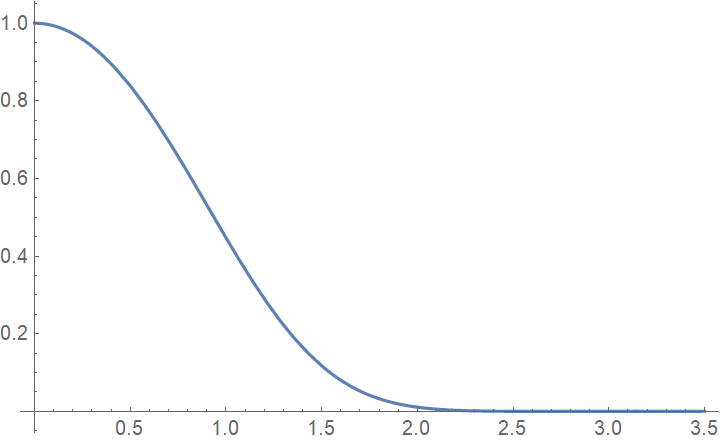
\includegraphics[scale=0.4]{P02/HO4.png}
\end{center}
\item
It appears that this wave-function looks like a gaussian, which is known to be the ground state of the simple harmonic oscillator potential. Thus, a good candidate wavefunction for the first excited state of this potential is the first excited state of the simple harmonic oscillator, 
\begin{equation}
	\braket{x}{\psi_\alpha}=u\exp(-\alpha u^2)\text{ where }\alpha>0, \alpha\in\mathbb R
\end{equation} 
Where $u\equiv\frac{x}{\beta}$. Show that all states $\ket{\psi_\alpha}$ are all orthogonal to the ground state
\begin{equation}
	\braket{0}{\psi_a}=\int_{-\infty}^\infty\braket{0}{u}\braket{u}{\psi_a}dx=\int_{-\infty}^\infty\braket{0}{u}u\exp(-\alpha u^2)dx
\end{equation} 
Note the ground state is even
\begin{equation}
	\braket{0}{\psi_a}=\int_0^\infty\braket{0}{u}u\exp(-\alpha u^2)du+\int_{-\infty}^0\braket{0}{u}u\exp(-\alpha u^2)du
\end{equation}
For the second term, let $k=-u$ then $dk=-du,u=-k,\braket{0}{k}=\braket{0}{x}, u^2=k^2$.
\begin{equation}
	\braket{0}{\psi_a}=\int_0^\infty\braket{0}{u}u\exp(-\alpha u^2)du+\int_{\infty}^0\braket{0}{k}k\exp(-\alpha k^2)dk
\end{equation} 
Re-substituting $u=k$.
\begin{equation}
	\braket{0}{\psi_a}=\int_0^\infty\braket{0}{u}u\exp(-\alpha u^2)du-\int_{0}^\infty\braket{0}{u}u\exp(-\alpha u^2)du=0
\end{equation}
Therefore, the variational principle can be applied to obtain a upper bound on the first excited state
\begin{equation}
	e_1\leq\frac{\bra{\psi_a}\hat h\ket{\psi_a}}{\braket{\psi_a}{\psi_a}}=\frac{2^\frac{5}{2}\alpha^\frac{3}{2}}{\sqrt\pi}\int_{-\infty}^\infty u\exp(-\alpha u^2)\left(-\frac{1}{2}\frac{d^2}{du^2}+u^4\right)\left(u\exp(-\alpha u^2)\right)
\end{equation}  
\begin{equation}
	=\frac{2^\frac{5}{2}\alpha^\frac{3}{2}}{\sqrt\pi}\int_{-\infty}^\infty \exp(-2\alpha u^2)\left(u^6-2a^2u^4+3au^2\right)du=\frac{2^\frac{5}{2}\alpha^\frac{3}{2}}{\sqrt{\pi}}\frac{3\sqrt{\pi}(5+8\alpha^3)}{2^\frac{13}{2}\alpha^\frac{7}{2}}=\frac{3}{16}(5\alpha^{-2}+8\alpha)
\end{equation} 
It is easy to see that the bound is concave for $\alpha>0$, thus, the stationary point will be the minimum point. Taking the derivative with respect to $\alpha$ yields
\begin{equation}
	\frac{3}{16}(-10\alpha^{-3}+8)=0
\end{equation}
\begin{equation}
	10=8\alpha^3\text{ so }\alpha=\frac{10^{\frac{1}{3}}}{2}\approx 1.07722\text{ and }\alpha^{-2}\approx 0.861774
\end{equation}   
The upper bound can be calculated to be $e_1\leq 2.423$.
\newpage
\item
The next lowest value of $e$ is about $2.394$. The wave function looks like this\\
\begin{center}
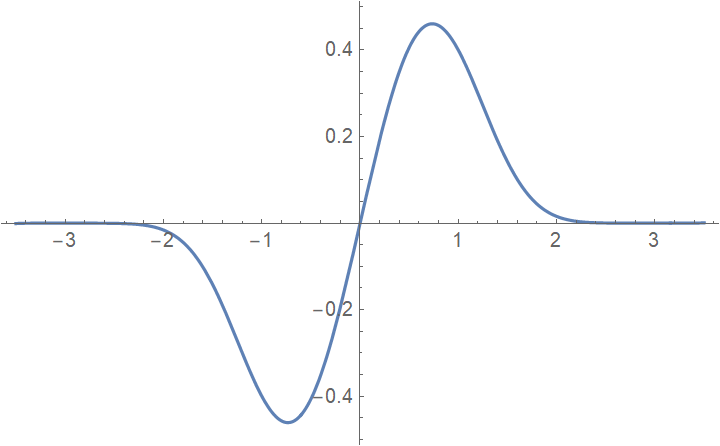
\includegraphics[scale=0.4]{P02/HO1.png}
\end{center}
\end{enumerate}
\end{sol}
    \begin{sol}
Notice the following about the matrix $\mathbf{M}$.
\begin{equation}
	\mathbf{MM}=\begin{pmatrix}0 & -i\\i&0\end{pmatrix}\begin{pmatrix}0 & -i\\i&0\end{pmatrix}=\begin{pmatrix}
1&0\\0&1
\end{pmatrix}\equiv\mathbf{1}
\end{equation} 
By definition, $\mathbf{1M}\equiv\mathbf{M}$ and $\mathbf{M}^1=\mathbf{M}$, it can be deduced by induction from $\mathbf{MM}=\mathbf{1}$ that
\begin{equation}
	\mathbf{M}^{2n}=\mathbf{1} \text{ and } \mathbf{M}^{2n+1}=\mathbf{M}\text{ for }n\in\mathbb{Z}
\end{equation}

Take the taylor expansion of $e^{iM\theta}$
\begin{equation}
	e^{iM\theta}=\sum_{n=0}^\infty\frac{i^n(\mathbf{M}\theta)^n}{n!}=1+i\mathbf{M}\theta-\frac{(\mathbf{M}\theta)^2}{2}-\frac{i(\mathbf{M}\theta)^3}{6}...
\end{equation} 
\begin{equation}
	=\sum_{n=0}^\infty(-1)^n\frac{\mathbf{M}^{2n}\theta^{2n}}{(2n)!}+i\sum_{n=0}^\infty(-1)^n\frac{\mathbf{M}^{2n+1}\theta^{2n+1}}{(2n+1)!}
\end{equation}
\begin{equation}
	=\mathbf{1}\sum_{n=0}^\infty(-1)^n\frac{\theta^{2n}}{(2n)!}+i\mathbf{M}\sum_{n=0}^\infty(-1)^n\frac{\theta^{2n+1}}{(2n+1)!}
\end{equation}
\begin{equation}
	=\cos(\theta)\mathbf{1}+i\sin(\theta)\mathbf{M}
\end{equation}
The algebraic property of any matrix that would lead to this result is the matrix is its own inverse.
\end{sol}
\newpage    
\section{Problem Set 3}
	\begin{sol}
\begin{enumerate}[label=\textbf{(\alph*)}]
\item
A general normalized spin state $\ket{\mathbf{n}(\theta,\phi);+}=\begin{pmatrix}\cos(\frac{\theta}{2})\\e^{i\phi}\sin(\frac{\theta}{2})\end{pmatrix}$\\
Let the positive $z$ axis be in the direction of $\ket{+}$ such that $\braket{z;+}{+}$= 1. The unnormalized spin state given is $\ket{\psi}=\begin{pmatrix}1+i\\-1-i\sqrt{3}\end{pmatrix}$ 
First, normalize the spin state in a way where the first component is real, as $\cos(\frac{\theta}{2})$ is real.
$$\braket{\psi}{\psi}=\begin{pmatrix}1-i & -1+i\sqrt{3}\end{pmatrix}\begin{pmatrix}1+i\\-1-i\sqrt{3}\end{pmatrix}=2+4=6$$
$$\ket\Psi=\frac{\ket\psi}{\sqrt{\braket{\psi}{\psi}}}=\frac{1}{\sqrt 6}\begin{pmatrix}1+i\\-1-i\sqrt{3}\end{pmatrix}$$
A factor of $1+i$ can be taken out to make the first component real
$$\ket\Psi=\frac{1+i}{\sqrt 6}\begin{pmatrix}1\\\frac{-1-i\sqrt 3}{1+i}\end{pmatrix}=e^{i\frac{\pi}{4}}\frac{1}{\sqrt{3}}\begin{pmatrix}1\\\frac{-1-\sqrt{3}}{2}+\frac{1-\sqrt{3}}{2}i\end{pmatrix}$$
$$\theta=2\cos^{-1}\left(\frac{1}{\sqrt{3}}\right)\approx 109.5\degree$$ 
$$\frac{1}{\sqrt 3}\left(\frac{-1-\sqrt{3}}{2}+\frac{1-\sqrt{3}}{2}i\right)=e^{i\phi}\frac{\sqrt{2}}{\sqrt{3}}$$
$$\frac{-1-\sqrt{3}}{2}+\frac{1-\sqrt{3}}{2}i=e^{i\phi}\sqrt{2}$$ 
$$\phi=\tan^{-1}\left(-\frac{1-\sqrt{3}}{1+\sqrt{3}}\right)=15\degree$$ 
The spin state is pointing towards the direction of $\theta\approx 109.5\degree$and $\phi=15\degree$.
\item
For $\phi=0$, the eigenstates can be written as
$$\ket{\mathbf{n}(\theta);+}=\begin{pmatrix}\cos\left(\frac{\theta}{2}\right)\\\sin\left(\frac{\theta}{2}\right)\end{pmatrix} \text{ and }\ket{\mathbf{n}(\theta);-}=\begin{pmatrix}\sin\left(\frac{\theta}{2}\right)\\-\cos\left(\frac{\theta}{2}\right)\end{pmatrix}$$  
Thus, the atoms which the second magnet are in the state $\ket{z;+}$. The probability of measuring spin-down in the direction of $\mathbf{n}$ is 
$$|\braket{\mathbf{n}(\theta);-}{z;+}|^2=\bigg|\begin{pmatrix}\sin\left(\frac{\theta}{2}\right)&-\cos\left(\frac{\theta}{2}\right)\end{pmatrix}\begin{pmatrix}1\\0\end{pmatrix}\bigg|^2=\sin^2\left(\frac{\theta}{2}\right)$$
The atoms that are blocked, therefore, never make it to the third magnet is $\sin^2(\frac{\theta}{2})$.\\
The particle entering the third slit is in the state $\braket{\mathbf{n}(\theta);+}{z;+}\ket{\mathbf{n}(\theta);+}$. The probability of it being measured to be in the state $\ket{z;+}$ is
$$|\braket{z;+}{\braket{\mathbf{n}(\theta);+}{z;+}\ket{\mathbf{n}(\theta);+}}|^2=\bigg|\cos\left(\frac{\theta}{2}\right)\begin{pmatrix}1&0\end{pmatrix}\begin{pmatrix}\cos\left(\frac{\theta}{2}\right)\\\sin\left(\frac{\theta}{2}\right)\end{pmatrix}\bigg|^2=\cos^4\left(\frac{\theta}{2}\right)$$

Through a similar process, the probability of the particle being measured to be in the state $\ket{z;-}$ is

$$|\braket{z;-}{\braket{\mathbf{n}(\theta);+}{z;+}\ket{\mathbf{n}(\theta);+}}|^2=\bigg|\cos\left(\frac{\theta}{2}\right)\begin{pmatrix}0&1\end{pmatrix}\begin{pmatrix}\cos\left(\frac{\theta}{2}\right)\\\sin\left(\frac{\theta}{2}\right)\end{pmatrix}\bigg|^2$$
$$=\left(\sin\left(\frac{\theta}{2}\right)\cos\left(\frac{\theta}{2}\right)\right)^2=\frac{1}{4}\sin^2(\theta)$$
For $\theta=0$, the expected probability to measure a particle in the state $\ket +$ is 1. The equations predicts the result correctly since $\cos^4(0)=1$, and $\sin^4(0)=0$.\\
For $\theta=\frac{\pi}{2}$, the particle should be blocked by the 2nd Stern-Garlach device with probability $\frac{1}{2}$. The equations predicts this result correctly since $\sin^2(\frac{\pi}{4})=\frac{1}{2}$. The particles that are not blocked should have equal probability to be measured as either $\ket+$ or $\ket-$. This is also correctly predicted by the equations since $\frac{1}{4}\sin^2(\frac{\pi}{2})=\cos^4(\frac{\pi}{2})=\frac{1}{4}$.\\
For $\theta=\pi$, all the particles should be blocked by the 2nd Stern-Garlach device. The equations also predicts this result correctly as $\sin^2(\frac{\pi}{2})=1$.
\end{enumerate}
\end{sol}
    \begin{sol}
It is well known that a state $\ket{\mathbf{n}(\theta,\phi);+}=\begin{pmatrix}\cos(\frac{\theta}{2})\\e^{i\phi}\sin(\frac{\theta}{2})\end{pmatrix}$ \\
\begin{equation}
	|\braket{\mathbf{n'}(\theta,\phi);+}{\mathbf{n}(\theta,\phi);+}|^2=\bigg|\begin{pmatrix}\cos\left(\frac{\theta'}{2}\right)&e^{-i\phi'}\sin\left(\frac{\theta'}{2}\right)\end{pmatrix}\begin{pmatrix}\cos\left(\frac{\theta}{2}\right)\\e^{i\phi}\sin\left(\frac{\theta}{2}\right)\end{pmatrix}\bigg|^2
\end{equation}
\begin{equation}
	=\bigg|\cos\left(\frac{\theta'}{2}\right)\cos\left(\frac{\theta}{2}\right)+e^{i(\phi-\phi')}\sin\left(\frac{\theta'}{2}\right)\sin\left(\frac{\theta}{2}\right)\bigg|^2
\end{equation}
\begin{equation}
	=\cos^2\left(\frac{\theta'}{2}\right)\cos^2\left(\frac{\theta}{2}\right)+\sin^2\left(\frac{\theta'}{2}\right)\sin^2\left(\frac{\theta}{2}\right)+2\cos\left(\frac{\theta'}{2}\right)\cos\left(\frac{\theta}{2}\right)\sin\left(\frac{\theta'}{2}\right)\sin\left(\frac{\theta}{2}\right)\cos(\phi-\phi')
\end{equation} 
\begin{equation}
	=\cos^2\left(\frac{\theta'}{2}\right)\cos^2\left(\frac{\theta}{2}\right)+\sin^2\left(\frac{\theta'}{2}\right)\sin^2\left(\frac{\theta}{2}\right)+\frac{1}{2}\sin\left(\theta'\right)\sin\left(\theta\right)\cos(\phi-\phi')
\end{equation}
\begin{equation}
	=\frac{1}{2}(\cos(\theta')\cos(\theta)+\sin(\theta')\sin(\theta)\cos(\phi-\phi')+1)
\end{equation} 
Let $\mathbf{n}$ be represented in spherical coordinates as $(1,\theta,\phi)$. Let $\mathbf{n'}$ be represented in spherical coordinates as $(1,\theta',\phi')$.\\\\
Then, $\mathbf{n}=\begin{pmatrix}\sin\theta\cos\phi\\\sin\theta\sin\phi\\\cos\theta\end{pmatrix}$ and $\mathbf{n'}=\begin{pmatrix}\sin\theta'\cos\phi'\\\sin\theta'\sin\phi'\\\cos\theta'\end{pmatrix}$
\begin{equation}
	\mathbf{n}\cdot\mathbf{n'}=\mathbf{n}^\dagger\mathbf{n}'
\end{equation}
\begin{equation}
	=\sin\theta\cos\phi\sin\theta'\cos\phi'+\sin\theta\sin\phi\sin\theta'\sin\phi'+\cos\theta\cos\theta'
\end{equation} 
\begin{equation}
	=\sin\theta\sin\theta'(\cos\phi\cos\phi'-\sin\phi\sin\phi')+\cos\theta\cos\theta'
\end{equation} 
\begin{equation}
	=\sin\theta\sin\theta'\cos(\phi-\phi')+\cos\theta\cos\theta'\equiv\cos\gamma
\end{equation} 
Notice this expression appears in the expression for $|\braket{\mathbf{n'}(\theta,\phi);+}{\mathbf{n}(\theta,\phi);+}|^2$. Substituting $\cos\gamma$ will yield:
\begin{equation}
	|\braket{\mathbf{n'}(\theta,\phi);+}{\mathbf{n}(\theta,\phi);+}|^2=\frac{1}{2}(\cos\gamma+1)=\cos^2\left(\frac{\gamma}{2}\right)
\end{equation} 
\end{sol}
    \begin{sol}
\begin{lemma}
$||\mathbf{n}||=1\implies(\mathbf{n}\cdot\mathbf{\sigma})^2=\mathbf{1}
$
\end{lemma}
\begin{proof} 
The definition of the Pauli Matrices $\mathbf{\sigma}$ from the spin operators is $\hat{S}_i=\frac{1}{2}\sigma_i$. The commutators of the spin operators are known as
$$[\hat{S}_i,\hat{S}_j]\equiv i\epsilon_{ijk}\hat{S}_k$$ 
From this definition, it can be concluded that
$$\frac{1}{2}^2[\sigma_i,\sigma_j]=\frac{1}{2}i\epsilon_{ijk}\sigma_k$$
$$[\sigma_i,\sigma_j]=2i\epsilon_{ijk}\sigma_k$$
Next, it can be shown that $(\sigma_i)^2=\mathbf{1}$ 
$$\mathbf{\sigma}_1\mathbf{\sigma}_1=\begin{pmatrix}0&1\\1&0\end{pmatrix}\begin{pmatrix}0&1\\1&0\end{pmatrix} =\begin{pmatrix}1 &0\\0&1\end{pmatrix}\equiv\mathbf{1}$$ $$\mathbf{\sigma}_2\mathbf{\sigma}_2=\begin{pmatrix}0&-i\\i&0\end{pmatrix}\begin{pmatrix}0&-i\\i&0\end{pmatrix} =\begin{pmatrix}1 &0\\0&1\end{pmatrix}\equiv\mathbf{1}$$ $$\mathbf{\sigma}_3\mathbf{\sigma}_3=\begin{pmatrix}1&0\\0&-1\end{pmatrix}\begin{pmatrix}1&0\\0&-1\end{pmatrix} =\begin{pmatrix}1 &0\\0&1\end{pmatrix}\equiv\mathbf{1}$$
Next, it can be shown that $\sigma_i\sigma_j=-\sigma_j\sigma_i$. Note only the case of $\sigma_1\sigma_2=-\sigma_2\sigma_1$ will be shown here, but the other cases can be computed and will satisfy this identity.
$$\sigma_1\sigma_2=\begin{pmatrix}0&1\\1&0\end{pmatrix}\begin{pmatrix}0&-i\\i&0\end{pmatrix}=\begin{pmatrix}i&0\\0&-i\end{pmatrix}$$ 
$$\sigma_2\sigma_1=\begin{pmatrix}0&-i\\i&0\end{pmatrix}\begin{pmatrix}0&1\\1&0\end{pmatrix}=\begin{pmatrix}-i&0\\0&i\end{pmatrix}=-\begin{pmatrix}i&0\\0&-i\end{pmatrix}$$ 
Thus, the anti-commutator $\{\sigma_i,\sigma_j\}=2\delta_{ij}\mathbf{1}$.\\\\
Given the definition of the commutator and anti-commutator, an operator product $AB=\frac{1}{2}([A,B]+\{A,B\})$. Thus,
$$\sigma_i\sigma_j=i\epsilon_{ijk}\sigma_k+\delta_{ij}\mathbf{1}$$
From the definition of the dot product and the cross product, $$a\cdot b=a_ib_i=a_ib_j\delta_{ij}$$ 
$$(a\times b)_k=a_ib_j\epsilon_{ijk}$$
Since the components of $\mathbf{n}$ are scalars, 
$$(\mathbf{n}\cdot\mathbf{\sigma})^2=(\mathbf{n}\cdot\mathbf{\sigma})(\mathbf{n}\cdot\mathbf{\sigma})=(n_i\sigma_i)(n_j\sigma_j)=i(n_in_j\epsilon_{ijk})\sigma_k+n_in_j\delta_{ij}\mathbf{1}$$ 
$$=i(\mathbf{n}\times\mathbf{n})\sigma_k+(\mathbf{n}\cdot\mathbf{n})\mathbf{1}=||\mathbf{n}||^2\mathbf{1}=\mathbf{1}$$
\end{proof}
\begin{enumerate}[label=\textbf{(\alph*)}]
\item
Define $\theta\equiv-\frac{\alpha}{2}$ and $\mathbf{M}\equiv\mathbf{n}\cdot\mathbf{\sigma} $. Note $$\hat{R_\mathbf{n}}(\alpha) = \exp(i\mathbf{M}\theta)$$
From Lemma 5 and the result from \textit{sol.6, p.16},
$$\hat{R_\mathbf{n}}(\alpha) =\cos(\theta)\mathbf{1}+i\sin(\theta)\mathbf{M}=\mathbf{1}\cos(\frac{\alpha}{2})-i\mathbf{\sigma}\cdot\mathbf{n}\sin(\frac{\alpha}{2})$$ The adjoint of $\hat{R_\mathbf{n}}$ is 
$$\hat{R_\mathbf{n}}(\alpha)^\dagger=\mathbf{1}\cos(\frac{\alpha}{2})+i(\mathbf{\sigma}\cdot\mathbf{n})^\dagger\sin(\frac{\alpha}{2})$$
Since $\mathbf{n}$ is a vector of scalars and every component of $\sigma$ is hermitian, $\mathbf{\sigma}\cdot\mathbf{n}$ must be hermitian. Thus, 
$$\hat{R_\mathbf{n}}(\alpha)^\dagger=\mathbf{1}\cos(\frac{\alpha}{2})+i\mathbf{\sigma}\cdot\mathbf{n}\sin(\frac{\alpha}{2})$$
$$\hat{R_\mathbf{n}}(\alpha)^\dagger\hat{R_\mathbf{n}}(\alpha)=(\mathbf{1}\cos(\frac{\alpha}{2})+i\mathbf{\sigma}\cdot\mathbf{n}\sin(\frac{\alpha}{2}))(\mathbf{1}\cos(\frac{\alpha}{2})-i\mathbf{\sigma}\cdot\mathbf{n}\sin(\frac{\alpha}{2}))$$ $$=\mathbf{1}\cos^2(\frac{\alpha}{2})+(\sigma\cdot\mathbf{n})^2\sin^2(\frac{\alpha}{2})$$ From Lemma 5, $(\sigma\cdot\mathbf{n})^2=\mathbf{1}$ Thus,
$$\hat{R_\mathbf{n}}(\alpha)^\dagger\hat{R_\mathbf{n}}(\alpha)=\mathbf{1}(\cos^2(\frac{\alpha}{2})+\sin^2(\frac{\alpha}{2}))=\mathbf{1}$$ Thus, $\hat{R_\mathbf{n}}(\alpha)$ is unitary.
\item
From the definition, 
$$\hat{R_\mathbf{y}}(\alpha)=\mathbf{1}\cos(\frac{\alpha}{2})-i\sigma_y\sin(\frac{\alpha}{2})$$
$$\hat{R_\mathbf{y}}(\alpha)^\dagger=\mathbf{1}\cos(\frac{\alpha}{2})+i\sigma_y\sin(\frac{\alpha}{2})$$
$$\hat{S}_z=\frac{1}{2}\sigma_z$$ $$\hat{R_\mathbf{y}}(\alpha)\hat{S_z}\hat{R_\mathbf{y}}(\alpha)^\dagger=(\mathbf{1}\cos(\frac{\alpha}{2})-i\sigma_y\sin(\frac{\alpha}{2}))(\frac{1}{2}\sigma_z)(\mathbf{1}\cos(\frac{\alpha}{2})+i\sigma_y\sin(\frac{\alpha}{2}))$$ $$=\frac{1}{2}\Big(\sigma_z\cos^2(\frac{\alpha}{2})+i\sigma_z\sigma_y\sin(\frac{\alpha}{2})\cos(\frac{\alpha}{2})-i\sigma_y\sigma_z\sin(\frac{\alpha}{2})\cos(\frac{\alpha}{2})+\sigma_y\sigma_z\sigma_y\sin^2(\frac{\alpha}{2})\Big)$$
$$=\sigma_z\cos^2(\frac{\alpha}{2})+\frac{1}{2}i[\sigma_z,\sigma_y]\sin(\alpha)+\sigma_y\sigma_z\sigma_y\sin^2(\frac{\alpha}{2})$$
The commutator $[\sigma_z,\sigma_y]$ is known to be $-2i\sigma_x$. Moreover,
$$\sigma_y\sigma_z\sigma_y=\begin{pmatrix}0&-i\\i&0\end{pmatrix}\begin{pmatrix}1&0\\0&-1\end{pmatrix}\begin{pmatrix}0&-i\\i&0\end{pmatrix}=\begin{pmatrix}-1&0\\0&1\end{pmatrix}=-\sigma_z$$ 
Substituting the results into the original equation,
$$\hat{R_\mathbf{y}}(\alpha)\hat{S_z}\hat{R_\mathbf{y}}(\alpha)^\dagger=\frac{1}{2}\Big(\sigma_z\cos^2(\frac{\alpha}{2})-\sigma_z\sin^2(\frac{\alpha}{2})+\sigma_x\sin(\alpha)\Big)$$
$$=\frac{1}{2}\big(\sigma_z\cos(\alpha)+\sigma_x\sin(\alpha)\big)$$ $$=\hat S_z\cos(\alpha)+\hat S_x\sin(\alpha)$$  
\item
$$\hat{R_\mathbf{y}}(\alpha)\ket{+}=\Big(\mathbf{1}\cos(\frac{\alpha}{2})-i\sigma_y\sin(\frac{\alpha}{2})\Big)\ket{+}$$ 
The state $\ket{+}$ can be represented by the column vector $\begin{pmatrix}1\\0\end{pmatrix}$.
$$\hat{R_\mathbf{y}}(\alpha)\begin{pmatrix}1\\0\end{pmatrix}=\cos(\frac{\alpha}{2})\begin{pmatrix}1&0\\0&1\end{pmatrix}\begin{pmatrix}1\\0\end{pmatrix}-i\sin(\frac{\alpha}{2})\begin{pmatrix}0&-i\\i&0\end{pmatrix}\begin{pmatrix}1\\0\end{pmatrix}=\begin{pmatrix}\cos(\frac{\alpha}{2})\\\sin(\frac{\alpha}{2})\end{pmatrix}$$ 
The resulting state is an eigenstate of the operator $\hat{R_\mathbf{y}}(\alpha)\hat{S_z}\hat{R_\mathbf{y}}(\alpha)^\dagger$ with eigenvalue $\frac{1}{2}$. Simply check this result by multiplying. Note that $$\hat{R_\mathbf{y}}(\alpha)\hat{S_z}\hat{R_\mathbf{y}}(\alpha)^\dagger=\hat S_z\cos(\alpha)+\hat S_x\sin(\alpha)=\frac{1}{2}\begin{pmatrix}\cos\alpha&\sin\alpha\\\sin\alpha&-\cos\alpha\end{pmatrix}$$
$$\hat{R_\mathbf{y}}(\alpha)\hat{S_z}\hat{R_\mathbf{y}}(\alpha)^\dagger\begin{pmatrix}\cos(\frac{\alpha}{2})\\\sin(\frac{\alpha}{2})\end{pmatrix}=\frac{1}{2}\begin{pmatrix}\cos\alpha&\sin\alpha\\\sin\alpha&-\cos\alpha\end{pmatrix}\begin{pmatrix}\cos(\frac{\alpha}{2})\\\sin(\frac{\alpha}{2})\end{pmatrix}$$
$$=\frac{1}{2}\begin{pmatrix}\cos(\alpha)\cos(\frac{\alpha}{2})+\sin(\alpha)\sin(\frac{\alpha}{2})\\\sin(\alpha)\cos(\frac{\alpha}{2})-\cos(\alpha)\sin(\frac{\alpha}{2})\end{pmatrix}=\frac{1}{2}\begin{pmatrix}\cos(\frac{\alpha}{2})\\\sin(\frac{\alpha}{2})\end{pmatrix}$$
From part b, it can be noticed that using $\hat R_y(\alpha)\hat S\hat R_y(\alpha)^\dagger$  rotated the spin operator about the y-axis by an angle $\alpha$. The $\hat R_y(\alpha)$ operator rotated the spinors y-axis by an angle $\alpha$ such that they are eigenvectors of $\hat R_y(\alpha)\hat S\hat R_y(\alpha)^\dagger$. Furthermore, $\hat R_\mathbf{n}(\alpha)$ is a unitary operator similar to the translation and momentum change operators that have been used. Therefore, it is intuitive to think of  $\hat R_\mathbf{n}(\alpha)$ as a rotation operator whose behavior on the spin operator and their eigenvectors suggests that it is a rotation operator about the axis of $\mathbf{n}$ for an angle $\alpha$.
\end{enumerate}
\end{sol}
    \begin{sol}
\begin{lemma}
$\mathbf{a}\cdot\mathbf{b}=(\mathbf{b}\cdot\mathbf{a})^*$
\end{lemma}
\begin{proof} 
$$\mathbf a^\dagger\mathbf b=\mathbf{a}_i^*\mathbf{b}_i$$
$$\mathbf b^\dagger\mathbf a=\mathbf{a}_i\mathbf{b}_i^*=(\mathbf a^*_i\mathbf b_i)^*$$
Note: for $\mathbf a, \mathbf b\in\mathbb{R}^n$, $\mathbf{a}\cdot\mathbf{b}=\mathbf{b}\cdot\mathbf{a}$.
\end{proof}
\begin{enumerate}[label=\textbf{(\alph*)}]
\item
$$f(\lambda)\equiv|\mathbf{a}-\lambda\mathbf{b}|^2\geq 0$$ 
$$=(\mathbf{a}-\lambda\mathbf{b})\cdot(\mathbf{a}-\lambda\mathbf{b})=(\mathbf{a}-\lambda\mathbf{b})^\dagger(\mathbf{a}-\lambda\mathbf{b})=(\mathbf{a}^\dagger-\lambda\mathbf{b}^\dagger)(\mathbf{a}-\lambda\mathbf{b})$$ 
$$=\mathbf{a}^\dagger\mathbf a+\lambda^2\mathbf b^\dagger \mathbf b-\lambda (\mathbf a^\dagger\mathbf b+\mathbf{ab}^\dagger)$$
Using Lemma 6,
$$f(\lambda)=|\mathbf{a}|^2+\lambda^2|\mathbf{b}|^2-2\lambda (\mathbf a\cdot\mathbf b)$$
Since $f$ is a quadratic function in $\lambda$ and $|\mathbf{a}|^2$ and $|\mathbf{b}|^2$ are strictly non-negative, the minimum point for $f$ is at $\lambda_{min}=\frac{\mathbf{a}\cdot\mathbf{b}}{|\mathbf{b}|^2}$. $$\because f(\lambda)\geq 0\forall x\in\mathbb{R}, f(\lambda_{min})\geq 0$$ 
$$\min_{\lambda}f(\lambda)\equiv f(\lambda_{min})=|\mathbf{a}|^2+\frac{(\mathbf{a}\cdot\mathbf{b})^2}{|\mathbf{b}|^2}-\frac{2(\mathbf{a}\cdot\mathbf{b})^2}{|\mathbf{b}|^2}\geq 0$$
$$|\mathbf{a}|^2|\mathbf{b}|^2-(\mathbf{a}\cdot\mathbf{b})^2\geq 0$$
$$|\mathbf{a}\cdot\mathbf{b}|^2\leq|\mathbf{a}||\mathbf{b}|$$ 
The Schwarz inequality is saturated when $\lambda=\lambda_{min}$ or when $\displaystyle{\mathbf{b}=\frac{\mathbf{a}\cdot\mathbf{b}}{|\mathbf b|^2}\mathbf{a}}$.
\begin{lemma}
Given $f(z):\mathbb{C}\to\mathbb{C}$ is a holomorphic function for $z\in\mathbb{C}$, $Re(z_0)\neq 0, Im(z_0)\neq 0$
$$\frac{\partial f}{\partial z_0}(w)=0 \text{ and }\frac{\partial f}{\partial z_0^*}(w)=0\implies w \text{ is a stationary point of }f$$
\end{lemma}
\begin{proof}
A stationary point of $f$ is defined to be a point $z$ where
$$\lim_{\delta z\to 0,\delta z\in\mathbb{C}} \frac{f(w+\delta z)-f(z)}{\delta w}=0$$
Let $\epsilon$ be a small real number and $u\in\mathbb C$. The equation above is equivalent to 
$$\lim_{\epsilon\to 0} \frac{f(w+u\epsilon)-f(w)}{u\epsilon}=0$$ 
This limit is also the definition of $\displaystyle{\frac{\partial f}{\partial u}}$. 
\\
$$\text{Re}(z_0)\neq 0, \text{Im}(z_0)\neq 0\implies\forall z\in\mathbb{C}=\alpha z_0+\beta z_0^*, (\alpha,\beta)\in\mathbb{R}^2$$
$$\therefore\frac{\partial f}{\partial u}=\alpha\frac{\partial f}{\partial z_0}+\beta\frac{\partial f}{\partial z_0^*}=0$$ 
Define $w=u\epsilon$ and the defining condition for a stationary point of $f$ is satisfied. 
\end{proof}
\item
$$f(\lambda)\equiv\braket{\nu(\lambda)}{\nu(\lambda)}\geq 0$$
$$=\braket{\ket a-\lambda\ket b}{\ket a-\lambda\ket b}=\braket{a}{a}+|\lambda|^2\braket{b}{b}-\lambda\braket{a}{b}-\lambda^*\braket{b}{a})$$ 
Using Lemma 6, 
$$f(\lambda)=|a|^2+|\lambda|^2|b|^2-2\lambda\braket{a}{b}=|a|^2+\lambda^*\lambda|b|^2-\lambda\braket{a}{b}+\lambda^*\braket{a}{b}^*$$
Since $f$ is a quadratic function in $\lambda$ and $\lambda^*$ and $\braket{a}{a}$ and $\braket{b}{b}$ are non-negative, the stationary point of $f$ is a global minimum, which can be found using Lemma 7.
$$\frac{\partial f}{\partial\lambda}=\lambda^*|b|^2-\braket{a}{b}=0$$ 
$$\frac{\partial f}{\partial\lambda^*}=\lambda|b|^2-\braket{a}{b}^*=0$$ 
$$\therefore\lambda_{min}=\frac{\braket{a}{b}^*}{|b|^2},\lambda^*_{min}=\frac{\braket{a}{b}}{|b|^2}$$
Note that $\lambda_{min}^*\lambda_{min}|b|^4=|\lambda_{min}|^2|b|^4=|\braket{a}{b}|^2$.
$$f(\lambda_{min})=|a|^2+\frac{|\braket{a}{b}|^2}{|b|^2}-\frac{|\braket{a}{b}|^2}{|b|^2}-\frac{|\braket{a}{b}|^2}{|b|^2}=|a|^2-\frac{|\braket{a}{b}|^2}{|b|^2}\geq 0$$
$$|\braket{a}{b}|^2\leq\braket{a}{a}\braket{b}{b}$$ 
\item
The \textit{triangle inequality} is $|a+b|\leq|a|+|b|$.\\
Squaring both sides of the inequality results in:
$$|a+b|^2=\braket{a+b}{a+b}=\braket{a}{a}+\braket{b}{b}+\braket{a}{b}+(\braket{a}{b})^*$$
$$=\braket{a}{a}+\braket{b}{b}+2\text{Re}(\braket{a}{b})$$ 
$$(|a|+|b|)^2=\braket{a}{a}+\braket{b}{b}+2\braket{a}{b}$$
$$\because\forall z\in\mathbb C, |\text{Re}(z)|\leq|z|, |a+b|^2\leq(|a|+|b|)^2$$ 
Then, the \textit{triangle inequality} will miraculously manifest from taking the square root of both sides.
\end{enumerate}
\end{sol}
    \begin{sol}
\begin{enumerate}[label=\textbf{(\alph*)}]
\item
\begin{theorem}
$$V=U_1\oplus W \text{ and }V=U_2\oplus W\implies U_1=U_2$$
\end{theorem}
\begin{proof}
Assume $\exists x\in U_1: x\notin U_2$. If $x\in W$, then $U_1$ and $W$ are not linearly independent sub-spaces since $\mathbf 0= x+(-1)x_w:x\in U_1,x_w\equiv x\in W$. Thus, if $x\in U_1, x\notin W$. \\
$\because V=U_2\oplus W$, $x\notin V\therefore x\notin U_1$.\\
This leads to contradiction, thus $\nexists x\in U_1: x\notin U_2, x\notin W$.\\\\
Similarly, assume $\exists y\in U_2:y\notin U_1$. If $y\in W$, then $U_2$ and $W$ are not linearly independent sub-spaces since $\mathbf 0= y+(-1)y_w:y\in U_2,y_w\equiv y\in W$. Thus, if $y\in U_2, y\notin W$\\
$\because V=U_1\oplus W$, $y\notin V\therefore y\notin U_2$.\\
This leads to contradiction, thus $\nexists y\in U_2: y\notin U_1, x\notin W$.\\\\
Therefore, $U_1=U_2$.
\end{proof}
\item
\begin{theorem}
The vector space composed of all infinite sequences $\mathbb F^\infty$ is infinite dimensional. 
\end{theorem}
\begin{proof}
Assume the $\mathbb F^\infty$ is finite dimensional. Using the result that in a finite dimensional vector space, the length of any spanning list must be larger or equal to the length of any list of linearly independent vectors. The following set of $N$ linearly independent vectors $S$ in $\mathbb F^\infty$ can be defined as $S(N)=\{v_i\}_{0\leq i<N}: v_i=\{a_j\}, a_j=\delta_{ij}$, where $N$ is an arbitrary finite integer. \\
It is trivial that $S$ is linearly independent as the unique way to represent $\textbf{0}$ in terms of linear combinations $v_i:v_i\in S(N)$ is $\mathbf 0=b_iv_i: b_i=0, b_i\in\mathbb F$.  If $\mathbb F^\infty$ is finite dimensional, there must exist a finite $N$ such that $S(N)$ spans $\mathbb F^\infty$. However, take the vector $u:u_i=\delta_{i,(N+1)}, u\in \mathbb F^\infty$ but there are no ways to represent $u$ as a linear combination of the elements of $S(N)$. $\therefore\nexists N:S(N)\text{ spans }\mathbb F^\infty$. Since $S(N)$ is linearly independent, there are no list shorter than $S(N)$ that spans $\mathbb F^\infty$. Thus, $\mathbb F^\infty$ is not finite dimensional.\\
By definition, if a vector space is not finite dimensional, it is infinite dimensional.
\end{proof}
\item
\begin{theorem}
A linear transformation $T$ is injective $\iff null(T)=\{0\}$
\end{theorem}
\begin{proof}
Let $T:\mathbb V\to\mathbb V$ where $\mathbb V$ is a vector space over $\mathbb F$.\\\\
Assume $\exists x\neq 0,x\in null(T)$. From linearity, $T(\alpha x+u)=T(u)\forall\alpha\in\mathbb F, u\in \mathbb V$. Therefore, there exists more than one vector in $\mathbb V$ where $T$ maps to the same point $T(u)$. By definition, $T$ cannot be injective. Moreover, $T$ is injective if and only if $null(T)=\{0\}$.
\end{proof}
\end{enumerate}
\end{sol}

    \begin{sol}
\begin{enumerate}[label=\textbf{(\alph*)}]
\item
Given $u_k=Av_k$ and $v_k=Bu_k$, the matrix representation of A is $u_j=A_{ij} v_i$ and the matrix representation of B is $v_j=B_{ij}u_i$. 
\\A and B are inverses since $ABu_k=A(Bu_k)=Av_k=u_k$ and $BAv_k=B(Av_k)=Bu_k=v_k$. Thus, $AB=BA=\mathbf{1}$, so $B=A^{-1}$ by definition.
\item
Using change of basis for matrices, $T_{ij}(\{u\})=A^{-1}T_{ij}(\{v\})A, T_{ij}(\{v\})=AT_{ij}(\{u\})A^{-1}$.
\item
Note the property of the identity $\mathbf{1}_{ij}=\delta_{ij}$. Thus, $A^{-1}_{ij}A_{jk}=A_{jk}A^{-1}_{ij}=\delta_{ik}$.
$$tr(T\{u\})\equiv T\{u\}_{ii}=(A^{-1}T\{v\}A)_{ii}$$ 
$$=A^{-1}_{ij}T\{v\}_{jk}A_{ki}=A^{-1}_{ij}A_{ki}T\{v\}_{jk}=\delta_{jk}T\{v\}_{jk}$$   
$$=T\{v\}_{jj}\equiv tr(T\{v\})$$  
\item
Using the identity $\det(AB)=\det(A)\det(B)$
$$\det(T\{u\})=\det(A^{-1}T\{v\}A)=\det(A^{-1})\det(T\{v\})\det(A)$$
$$=\det(A^{-1}A)\det(T\{v\})=\det(\mathbf{1})\det(T\{v\})=\det(T\{v\})$$ 

\end{enumerate}
\end{sol}
\newpage
\section{Problem Set 4}
	\begin{sol}
\begin{enumerate}[label=\textbf{(\alph*)}]
\item
$$[A,BC]=ABC-BCA=ABC-B(AC-(AC-CA))$$$$=ABC-BAC+B[A,C]=[A,B]C+B[A,C]$$
\item
$$[[A,B],C]+[[B,C],A]+[[C,A],B]=[AB-BA,C]+[BC-CB,A]+[CA-AC,B]$$ 
$$=ABC-CAB-BAC+CBA+BCA-ABC-CBA+ACB+CAB-BCA-ACB+BAC$$ 
$$=0$$ \item
$$[q^n,p]=-[p,qq^{n-1}]=-([p,q]q^{n-1}+q[p,q^{n-1}])=[q,p]q^{n-1}+q[q^{n-1},p]=iq^{n-1}+q[q^{n-1},p]$$
Assume the identity $[q^n,p]=inq^{n-1}$ is true.
$$inq^{n-1}=iq^{n-1}+qi(n-1)q^{n-2}$$ $$inq^{n-1}=inq^{n-1}$$
\item
Given $f(q)$ can be expanded in a power series of $q$, define $a_n:f(q)=\sum_{n=0}^\infty a_nq^n$
$$[f(q),p]=\sum_{n=0}^\infty[a_nq^n,p]=i\sum_{n=0}^\infty a_nnq^{n-1}$$ 
Take the derivative of the power series of $f(q)$ using the power rule for derivatives
$$f'(q)=\sum_{n=0}^\infty a_n nq^{n-1}\therefore[f(q),p]=if'(q)$$
\item
Let the commutator act of an arbitrary wavefunction $\psi$.
$$[f(x),p]\psi=f(x)\left(-i\frac{\partial}{\partial x}\right)\psi-\left(-i\frac{\partial}{\partial x}\right)f(x)\psi$$
$$=-if(x)\frac{\partial\psi}{\partial x}+if'(x)\psi+if(x)\frac{\partial\psi}{\partial x}=if'(x)\psi$$ $$\therefore[f(x),p]=if'(x)$$ 
\end{enumerate}
\end{sol}
    \newpage
\begin{sol}
\begin{enumerate}[label=\textbf{(\alph*)}]
\item
Using the formal definition of the exponential, 
$$e^{x}=\sum_{n=0}^\infty\frac{x^n}{n!}$$ 
Thus, the derivative of the exponential is
$$\frac{d}{dt}e^x=\sum_{n=0}^\infty\frac{dx}{dt}\frac{nx^{n-1}}{n!}=\frac{dx}{dt}\sum_{n=0}^\infty\frac{x^n}{n!}=\frac{dx}{dt}e^x$$ 
Also, note the following
$$[e^{tL},L]=\sum_{n=0}^\infty\frac{t^nL^n}{n!}L-L\sum_{n=0}^\infty\frac{t^nL^n}{n!}=\sum_{n=0}^\infty \frac{t^n}{n!}(L^nL-LL^n)=0$$
Letting $x=tL$ and $L=A+B$, it becomes trivial that
$$\frac{d}{dt}e^{t(A+B)}=(A+B)e^{t(A+B)}=e^{t(A+B)}(A+B)$$
\item
\begin{lemma}
$$[A,B]=c: c=\kappa\mathbf 1, \kappa\in\mathbb C\implies e^ABe^{-A}=B+c$$
\end{lemma}
\begin{proof}
Let $F(t)=e^{tA}Be^{-tA}$. It is trivial that $F(0)=B$.
$$\frac{dF}{dt}=Ae^{tA}Be^{-tA}+e^{tA}B(-Ae^{-tA})$$ $$=e^{tA}ABe^{-tA}-e^{tA}BAe^{-tA}=e^{tA}[A,B]e^{-tA}=e^{tA}ce^{-tA}=c$$
Note that $e^ABe^{-A}=F(1)$
$$F(t)=F(0)+\int_0^t\frac{dF}{dt}dt=F(0)+ct|_0^t=B+ct$$ 
$$F(1)=B+c$$ 
\end{proof}
\item
First, note that the translation operator can be written as $\hat T=e^{-A}, A=ia\hat p$.\\
Compute the commutator $[A,\hat x]=ia[p,x]=a$. Also note that $\hat{ T^\dagger}=e^A\therefore\hat{ T^\dagger}(a)\hat x\hat T(a)=e^A\hat x e^{-A}$. Applying Lemma 8 yields $\hat{ T^\dagger}(a)\hat x\hat T(a)=\hat x+a$\\\\
Given $\braket{x}{\psi}=\psi(x)$, $\bra x\hat T(a)=\bra{\hat T(a)^\dagger x}=\bra{x-a}$
$$\bra x\hat T(a)\ket\psi=\braket{x-a}{\psi}=\psi(x-a)$$
\end{enumerate}
\end{sol}
    \begin{sol}
\begin{theorem}
For any two operators $A$ and $B$; define $W_0=B, W_{n+1}=[A,W_n]$,
\begin{equation}
	e^ABe^{-A}=\sum_{n=0}^\infty\frac{W_n}{n!}=B+[A,B]+\frac{1}{2}[A,[A,B]]+\frac{1}{6}[A,[A,[A,B]]]+...
\end{equation} 
\end{theorem}
\begin{proof}
Since commutator expressions will be common, define
\begin{equation}
	\text{ad } A(X)\equiv[A,X]\therefore W_{n+1}=\text{ad }  A(W_n)
\end{equation}
\begin{equation}
	W_n=\text{ad }A^n(B)
\end{equation}
Define $f(t)=e^{tA}Be^{-tA}$. Since $f(t)$ is analytic at $t=0$, it can be expanded as a Taylor series.
\begin{equation}
	f(t)=\sum_{n=0}^\infty \frac{t^n}{n!}\frac{d^nf(t)}{dt^n}=f(0)+f'(0)t+\frac{1}{2}f''(0)t^2+\frac{1}{6}f'''(0)t^3+...
\end{equation} 
Note the first term is $f(0)=1$. The second term can be computed using the product rule.
\begin{equation}
	\frac{df}{dt}=Ae^{tA}Be^{-tA}+e^{tA}B(-Ae^{-tA})
\end{equation} \begin{equation}
	=e^{tA}ABe^{-tA}-e^{tA}BAe^{-tA}=e^{tA}[A,B]e^{-tA}=e^{tA}\text{ ad }A(B)e^{-tA}
\end{equation} 
Taking another derivative will yield
\begin{equation}
	\frac{d}{dt}\left(\frac{df}{dt}\right)=e^{tA}A\text{ ad }A(B)e^{-tA}-e^{tA}\text{ ad }A(B)Ae^{-tA}
\end{equation} 
\begin{equation}
	=e^{tA}[A,\text{ad }A(B)]e^{-tA}=e^{tA}\text{ ad }A^2(B)e^{-tA}
\end{equation}  
Given 
\begin{equation}
	\frac{d^nf}{dt^n}=e^{tA}\text{ ad }A^n(B)e^{-tA}
\end{equation}
\begin{equation}
	\frac{d^{n+1}f}{dt^{n+1}}=\frac{d}{dt}\left(\frac{d^nf}{dt^n}\right)=\frac{d}{dt}\left(e^{tA}\text{ ad }A^n(B)e^{-tA}\right)
\end{equation}
\begin{equation}
	=e^{tA}A\text{ ad }A^{n}(B)e^{-tA}-e^{tA}\text{ ad }A^{n}(B)Ae^{-tA}
\end{equation} 
\begin{equation}
	=e^{tA}[A,\text{ad }A^{n}(B)]e^{-tA}=e^{tA}\text{ ad }A^{n+1}(B)e^{-tA}
\end{equation}
Therefore, by induction, it is shown that 
\begin{equation}
	\frac{d^nf}{dt^n}=e^{tA}\text{ ad }A^n(B)e^{-tA}=e^{tA}W_ne^{-tA}
\end{equation}
The specific case of interest is $t=1$, where 
\begin{equation}
	f(1)=e^{A}Be^{-A}=\sum_{n=0}^\infty\frac{W_n}{n!}
\end{equation}
\end{proof}
\end{sol}
    \begin{sol}
\begin{enumerate}[label=\textbf{(\alph*)}]
\item
Define $G(t)\equiv e^{t(A+B)}e^{-tA}$,
\begin{equation}
	G^{-1}(t)=e^{tA}e^{-t(A+B)}
\end{equation}
\begin{equation}
	\frac{d}{dt}G(t)=e^{t(A+B)}(A+B)e^{-tA}-e^{t(A+B)}Ae^{-tA}=e^{t(A+B)}Be^{-tA}
\end{equation}
\begin{equation}
	G^{-1}\frac{d}{dt}G(t)=e^{tA}e^{-t(A+B)}e^{t(A+B)}Be^{-tA}=e^{tA}Be^{-tA}
\end{equation}
Using Lemma 8, 
\begin{equation}
	G^{-1}\frac{d}{dt}G(t)=B+ct
\end{equation} 
\item
\begin{equation}
	G(t)=G(0)e^{tB}e^{\frac{1}{2}ct^2}
\end{equation}
\begin{equation}
	\frac{d}{dt}G(t)=G(0)(Be^{tB}e^{\frac{1}{2}ct^2}+e^{tB}ct\,e^{\frac{1}{2}ct^2})
\end{equation}
It has been shown in \textit{2(a), p.29} that $[e^{tL},L]=0$. 
\begin{equation}
	\frac{d}{dt}G(t)=G(0)(e^{tB}e^{\frac{1}{2}ct^2})(B+ct)=G(t)(B+ct)
\end{equation}
\item
\begin{equation}
	G(1)\equiv e^{A+B}e^{-A}=G(0)e^Be^{c/2}
\end{equation}
\begin{equation}
	e^{A+B}=e^Be^Ae^{c/2}
\end{equation} 
Note that $[B,A]=-[A,B]$, thus $e^{A+B}=e^{B+A}=e^Ae^Be^{-c/2}$
\end{enumerate}
\end{sol}
    \begin{sol}
\begin{enumerate}[label=\textbf{(\alph*)}]
\item
The bras are the conjugate transpose of the kets:
\begin{equation}
	\bra{\psi}=a^*\bra{1}-b^*\bra{2}+a^*\bra{3};\,\,\,\,\,\bra{\phi}=b^*\bra 1+a^*\bra 2
\end{equation}
Owing to the orthonormal basis, $\braket{m}{n}=\delta_{mn}$
\begin{equation}
	\braket{\phi}{\psi}=(b^*\bra 1+a^*\bra 2)(a\ket 1-b\ket 2+a\ket 3)=ab^*-a^*b
\end{equation}
\begin{equation}
	\braket{\psi}{\phi}=(a^*\bra{1}-b^*\bra{2}+a^*\bra{3})(b\ket 1+a\ket 2)=a^*b-ab^*=\braket{\phi}{\psi}^*
\end{equation}
\item
\begin{equation}
	\ket\psi=\begin{pmatrix}a\\-b\\a\end{pmatrix}\,\,\,\,\,\ket\phi=\begin{pmatrix}b\\a\\0\end{pmatrix}
\end{equation}
\begin{equation}
	\bra{\psi}=\begin{pmatrix}a^*&-b^*&a^*\end{pmatrix}\,\,\,\,\,\bra\phi=\begin{pmatrix}b^*&a^*&0\end{pmatrix}
\end{equation} 
\begin{equation}
	\braket{\phi}{\psi}=\begin{pmatrix}b^*&a^*&0\end{pmatrix}\begin{pmatrix}a\\-b\\a\end{pmatrix}=ab^*-a^*b
\end{equation}
\begin{equation}
	\braket{\psi}{\phi}=\begin{pmatrix}a^*&-b^*&a^*\end{pmatrix}\begin{pmatrix}b\\a\\0\end{pmatrix}=a^*b-ab^*=\braket{\phi}{\psi}^*
\end{equation} 
\item
The general ket-bra matrix can be constructed as follows. \\
Define

\begin{equation}
	\ket v\equiv\ketbra{a}{b}\ket{u}=\braket{b}{u}\ket{a}
\end{equation} 
\begin{equation}
	\ket v_j=\ketbra{a}{b}_{ij}\ket{u}_i=\ket a_j\bra b_i\ket u_i
\end{equation} 
From the matrix representation of an operator, $T_{ij}\ket u_i=\ket v_j\therefore\ketbra{a}{b}_{ij}=\ket a_j\bra b_i$.


\begin{equation}
	A=\ketbra{\phi}{\psi}=\begin{pmatrix}
a^*b&-b^*b&a^*b\\
a^*a&-b^*a&a^*a\\
0&0&0 
\end{pmatrix}=\begin{pmatrix}
a^*b&-|b|^2&a^*b\\
|a|^2&-ab^*&|a|^2\\
0&0&0 
\end{pmatrix}
\end{equation}
\item 
The defining property of hermitian matrices is $Q=Q^\dagger$. Note this implies the following condition on its components $Q_{ij}=Q_{ji}^*$ due to the action of the definition of the conjugate transpose operation.\\
Shown above, if $P=\ketbra{\psi}{\psi}, P_{ij}=\ket\psi_j\bra\psi_i=\ket\psi_i^*\ket\psi_j$. From this, it is trivial that for any $\psi$, $P$ will be hermitian. Furthermore, the set of hermitian matrices is closed under linear combinations, thus $Q$ must be hermitian.
\begin{equation}
	\because Q:\mathbb C^3\to\mathbb C^3\exists\ket{\chi}\in\mathbb C^3:\braket{\phi}{\chi}=\braket{\psi}{\chi}=\mathbf 0\implies Q\ket{\chi}=\mathbf{0}=0\ket{\chi}
\end{equation}  
By definition, $\ket{\chi}$ is an eigenvector of $Q$ with zero eigenvalue.
\end{enumerate}
\end{sol}
    \begin{sol}
\begin{enumerate}
\item[\textbf{(1)}]
\begin{equation}
	\{M^i,M^j\}=2\delta^{ij}\mathbf{1}\implies M^iM^i=\mathbf{1}
\end{equation}  
Firstly, the eigenvalue of $(M^i)^2$ must be 1 since it is identical to the identity, which by definition, has all vectors as eigenvectors with eigenvalue 1. 
Let $\ket\phi$ be an eigenvector of $M^i$ with eigenvalue $\lambda$, then, $(M^i)^2\ket\phi=\lambda^2\ket\phi$. Since it has been shown that the eigenvalues of $(M^i)^2$ must be $1$, $\lambda^2=1$ thus $\lambda=\pm 1$.
\item[\textbf{(2)}]
\begin{equation}
	\{M^i,M^j\}=2\delta^{ij}\mathbf{1}\implies M^iM^j=-M^jM^i\text{ for }i\neq j
\end{equation}
As it is known that $M^iM^i=\mathbf{1}$, thus, $M^i$ must be invertible.
\begin{equation}
	M^i=-M^jM^i(M^j)^{-1}\text{ for }i\neq j
\end{equation}
\begin{equation}
	\Tr(M^i)=M^i_{nn}=-(M^jM^i(M^j)^{-1})_{nn}=-(M^j_{nl}M^i_{lm}(M^j)^{-1}_{mn})
\end{equation}
\begin{equation}
	=-((M^j)^{-1}_{mn}M^j_{nl}M^i_{lm})=-\mathbf 1_{ml}M^i_{lm}=-M^i_{ll}=-\Tr(M^i)
\end{equation}
It is shown that $\Tr(M^i)=-\Tr(M^i)$, thus, $M^i$ must be traceless.\\\\Note that the choice of $M^j$ is irrelevant to the problem and for any invertible matrix $S$, $\Tr(M)=\Tr(SMS^{-1})$. This fact will be used later.
\item[\textbf{(3)}]
It is shown that all matrices that satisfy the relation $\{M^i,M^j\}=2\delta^{ij}\mathbf{1}$ must be traceless and be its own inverse.\\
Assume there exists a set of four matrices that are odd dimensional which satisfies these relations. All matrices can be factored in the form of $M^i=S^iJ^i(S^i)^{-1}$, where $J^i$ is the matrix for $M^i$ written in Jordon canonical form. In this form, the diagonals are the eigenvalues of the matrix. Thus, $\Tr(M^i)=\Tr(S^iJ^i(S^i)^{-1})=\Tr(J^i)=0$. This is a sum of eigenvalues. However, it has also been shown that all eigenvalues of $M^i$ must be either $-1$ and $1$, which are both odd numbers. It is also well known that a sum of a odd amount of odd numbers is a odd number. Thus, for a odd-dimensional matrix the trace must be an odd number. However, zero is not an odd number, which is a contradiction. Therefore, there are no odd set of odd-dimensional matrices that satisfy $\{M^i,M^j\}=2\delta^{ij}\mathbf{1}$.
\end{enumerate}
\end{sol}
    \begin{sol}
\begin{enumerate}[label=\textbf{(\alph*)}]
\item
\begin{equation}
	\forall u\in\mathbb U, |v-u|\geq|v-P_U v|
\end{equation} 
The orthogonal projector acting on a vector $v=u+w, u\in\mathbb U, w\in\mathbb U^\perp$ will result in $P_Uv=u$.
\begin{equation}
	\braket{v-u}{v-u}\geq\braket{v-P_Uv}{v-P_Uv}
\end{equation}
\begin{equation}
	\braket{v}{v}+\braket{u}{u}-\braket{u}{v}-\braket{v}{u}\geq\braket{v}{v}+\braket{P_Uv}{P_Uv}-\braket{P_Uv}{v}-\braket{v}{P_Uv}
\end{equation}
\begin{equation}
	\braket{u}{u}-2\mathrm{Re}\braket{u}{v}\geq\braket{P_Uv}{P_Uv}-2\mathrm{Re}\braket{P_Uv}{v}
\end{equation}
Rewrite $v=P_uv+w, w\in\mathbb U^\perp$
\begin{equation}
	\braket{u}{u}-2\mathrm{Re}\braket{u}{P_Uv+w}\geq\braket{P_Uv}{P_Uv}-2\mathrm{Re}\braket{P_Uv}{P_Uv+w}
\end{equation}
\begin{equation}
	\braket{u}{u}-2\mathrm{Re}\braket{u}{P_Uv}-2\mathrm{Re}\braket{u}{w}\geq\braket{P_Uv}{P_Uv}-2\mathrm{Re}\braket{P_Uv}{P_Uv}-2\mathrm{Re}\braket{P_Uv}{w}
\end{equation}
The inner product of a vector with itself must be real, thus, $\mathrm{Re}\braket{v}{v}=\braket{v}{v}$.
\begin{equation}
	\braket{u}{u}-2\mathrm{Re}\braket{u}{P_Uv}\geq-\braket{P_Uv}{P_Uv}
\end{equation}
\begin{equation}
	\braket{u}{u}-2\mathrm{Re}\braket{u}{P_Uv}+\braket{P_Uv}{P_Uv}\geq 0
\end{equation}
\begin{equation}
	|u-P_Uv|^2\geq 0
\end{equation} 
\item
Let $\ket{e_1}= \alpha\ket{1}$
\begin{equation}
	\braket{e_1}{e_1}=1\implies \alpha^2\int_{-\pi}^\pi dx=1, 2\pi\alpha^2=1
\end{equation} \begin{equation}
	\alpha=\frac{1}{\sqrt{2\pi}}
\end{equation} \begin{equation}
	\ket{e_1}=\frac{1}{\sqrt{2\pi}}\ket 1
\end{equation}
\begin{equation}
	\ket{e_2}=\frac{\ket x-\braket{e_1}{x} \ket{e_1}}{|\ket x-\braket{e_1}{x} \ket{e_1}|}
\end{equation}
\begin{equation}
	\braket{e_1}{x}=\int_{-\pi}^\pi \frac{x}{\sqrt{2\pi}}=0
\,\,\,\,\,\, \braket{x}{x}=\int_{-\pi}^\pi x^2 dx=\frac{2\pi^3}{3}
\end{equation}\begin{equation}
	\ket{e_2}=\sqrt{\frac{3}{2\pi^3}}\ket x
\end{equation} 
The similar procedure can be applied to obtained $\ket{e_3}...\ket{e_6}$ to obtain
\begin{equation}
	\ket{e_3}=\sqrt{\frac{5}{8\pi^5}}(3\ket{x^2}-\pi^2\ket 1)
\end{equation}
\begin{equation}
	\ket {e_4}=\frac{25}{2}\sqrt{\frac{7}{2\pi^7}}(5\ket{x^3}-3\pi^2\ket x)
\end{equation} \begin{equation}
	\ket{e_5}=\frac{3}{8\sqrt{2\pi^9}}(35\ket{x^4}-30\pi^2\ket{x^2}+3\pi^4\ket 1)
\end{equation} 
\begin{equation}
	\ket{e_6}=\frac{1}{8}\sqrt{\frac{11}{2\pi^{11}}}(63\ket{x^5}-70\pi^2\ket{x^3}+15\pi^4\ket{x})
\end{equation} 
\item
\begin{equation}
	\ket{\sin x}\approx(\ketbra{e_1}{e_1}+\ketbra{e_2}{e_2}+...+\ketbra{e_6}{e_6})\ket{\sin x}
\end{equation} \begin{equation}
	=\frac{21x}{8\pi^{10}}\Big(33x^4(\pi^4-105\pi^2+945)-30\pi^2x^2(\pi^4-125\pi^2+1155)+5\pi^4(\pi^4-153\pi^2+1485)\Big)
\end{equation}
\begin{equation}
	\approx 0.00564312x^5-0.155271x^3+0.987862x
\end{equation} \begin{equation}
	\ket{\cos x}\approx(\ketbra{e_1}{e_1}+\ketbra{e_2}{e_2}+...+\ketbra{e_6}{e_6})\ket{\cos x}
\end{equation}\begin{equation}
	=\frac{105}{8\pi^8}\Big(315 x^4 - 30 \pi^2 x^2 (9 + x^2) + 3 \pi^4 (9 + 8 x^2)-2 \pi^6\Big)
\end{equation} \begin{equation}
	\approx 0.0261598x^4-0.452288x^2+0.978326
\end{equation} 
\item 
Plot of $\sin x$: Green-second degree, Yellow-fourth degree, Red-fifth degree, Blue-actual\\
\begin{center}
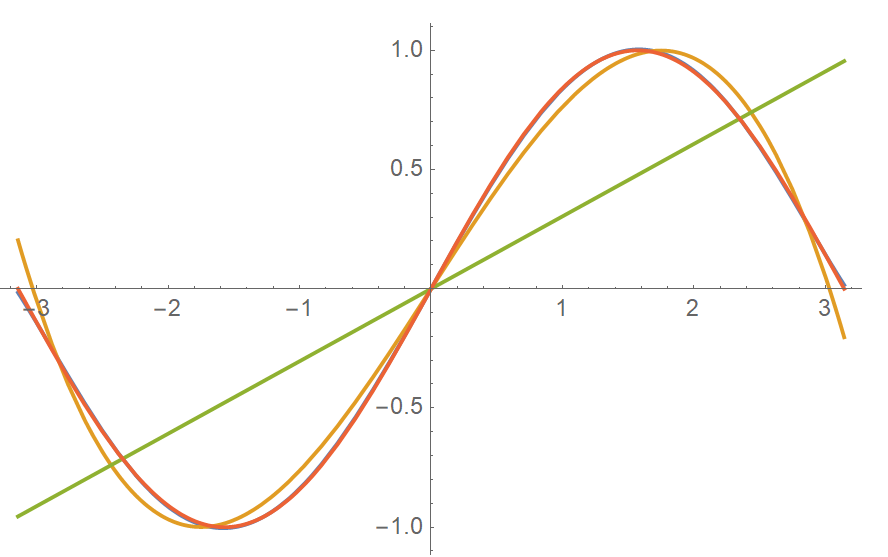
\includegraphics[scale=0.7]{P04/sinx.PNG}
\end{center}
Error (fifth degree): Blue-approximation in $\mathbb U$, yellow-taylor polynomial
\begin{center}
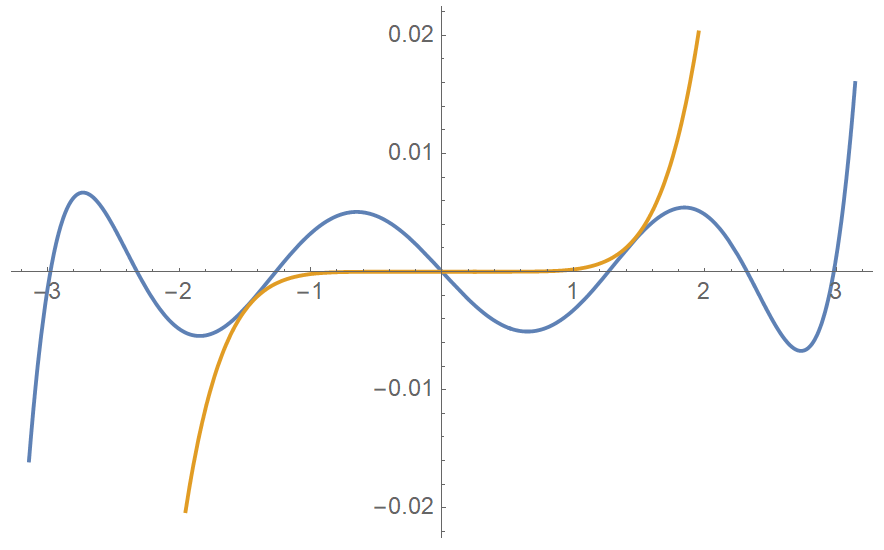
\includegraphics[scale=0.7]{P04/sin error.PNG}
\end{center}
Plot of $\cos x$: Yellow-third degree, Green-fifth degree, Blue-actual
\begin{center}
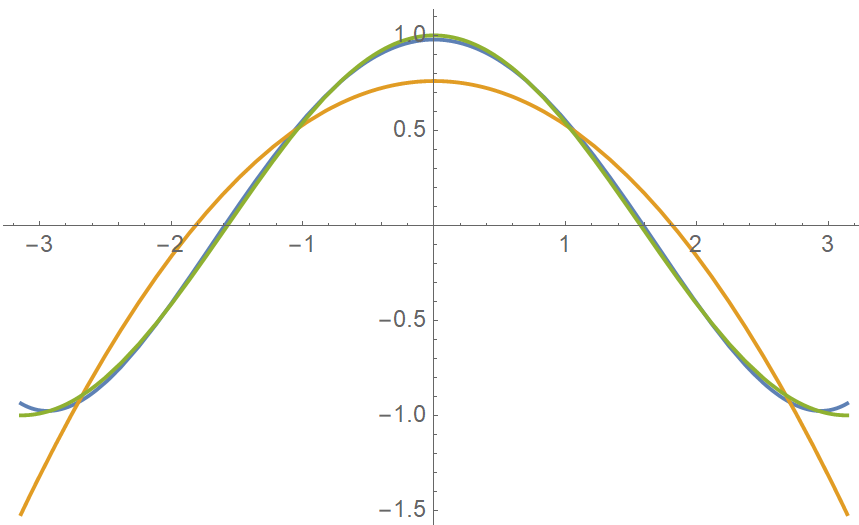
\includegraphics[scale=0.7]{P04/cosx.PNG}
\end{center}
\newpage
Error (fifth degree): Blue-approximation in $\mathbb U$, yellow-taylor polynomial
\begin{center}
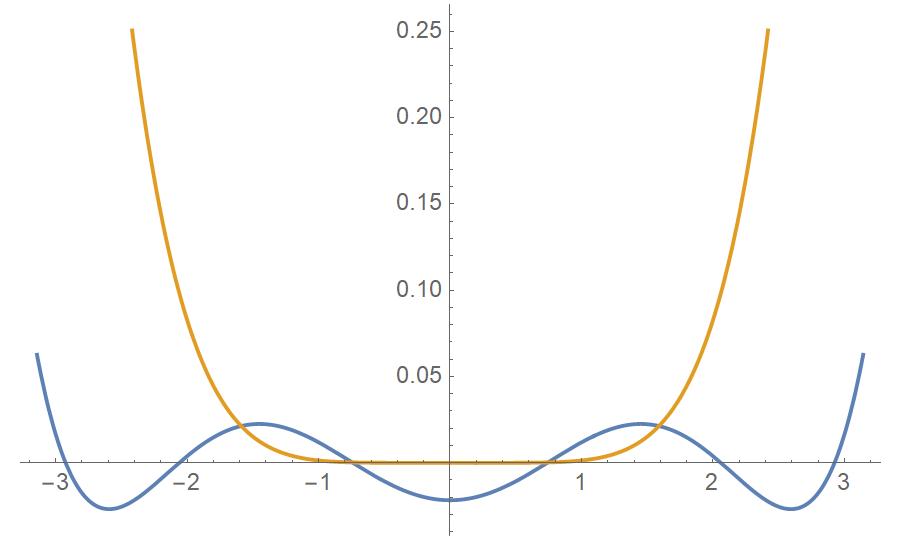
\includegraphics[scale=0.7]{P04/cos error.PNG}
\end{center}
In conclusion, the approximation in the space $\mathbb U$ is a better approximation if the entire interval $(-\pi,\pi)$ is considered whereas the taylor polynomial is a better approximation near zero. 

\end{enumerate}
\end{sol}
\newpage    
\section{Problem Set 5}
\begin{sol}
\begin{enumerate}[label=\textbf{(\alph*)}]
\item
Note that $[\hat x,\hat p]=i\mathbf{1}$. Applying Lemma 8 yields
\begin{equation}
	T_x^\dagger\hat xT_x=e^{i\hat p x}\hat xe^{-i\hat px}=\hat x+ix[\hat p,\hat x]\mathbf{1}=\hat x+x\mathbf{1}
\end{equation}
\begin{equation}
	\tilde T_p^\dagger\hat p\tilde T_p=e^{-ip\hat x}\hat pe^{ip\hat x}=\hat p-ip[\hat x,\hat p]=\hat p+p\mathbf{1}
\end{equation}
\item
Define the following intermediate operators: $A\equiv-i\hat p x, B\equiv ip\hat x$.
\begin{equation}
	[T_x,\tilde T_p]=T_x\tilde T_p-\tilde T_pT_x=e^{A}e^{B}-e^{B}e^{A}
\end{equation}
The commutator 
\begin{equation}
	[A,B]=xp[\hat p,\hat x]=-ixp\mathbf{1}
\end{equation} 
Since the commutator is a scalar multiple of the identity, the terms of the equation can be multiplied by the scalar $1=e^{-\frac{1}{2}[A,B]}e^{\frac{1}{2}[A,B]}$ 
\begin{equation}
	[T_x, \tilde T_p]=(e^Ae^Be^{-\frac{1}{2}[A,B]})e^{\frac{1}{2}[A,B]}-(e^Be^Ae^{\frac{1}{2}[A,B]})e^{-\frac{1}{2}[A,B]}
\end{equation}
Using the \textit{Baker-Campbell-Hausdorff Theorem} can simplify the bracketed expression to $e^{A+B}$, which can be factored out.
\begin{equation}
	[T_x, \tilde T_p]=e^{A+B}(e^{\frac{1}{2}[A,B]}-e^{-\frac{1}{2}[A,B]})=e^Ae^Be^{-\frac{1}{2}[A,B]}(e^{\frac{1}{2}[A,B]}-e^{-\frac{1}{2}[A,B]})=e^Ae^B(1-e^{-[A,B]})
\end{equation} The original operators can be substituted back in
\begin{equation}
	[T_x, \tilde T_p]=T_x\tilde T_p(1-e^{ixp})
\end{equation} 
Since neither $T_x$ and $\tilde T_p$ are not the zero operator, for the commutation relation to be zero, the following equation must be satisfied
\begin{equation}
	1-e^{ixp}=0
\end{equation}
Using \textit{Euler's Formula}
\begin{equation}
	1=\cos(xp)+i\sin(xp)
\end{equation} 
\begin{equation}
	xp=2\pi N: N\in\mathbb Z
\end{equation} 
\end{enumerate}
\end{sol}
\begin{sol}
\begin{enumerate}[label=\textbf{(\alph*)}]
\item
Apply the identity operator $\mathbf{1}=\int\ketbra{p}{p}dp$ 
$$\bra x\hat p^n\ket\psi=\int\bra x\hat p^n\ketbra{p}{p}\ket\psi dp=\int p^n\braket{x}{p}\braket{p}{\psi}dp$$  It is known that 
$$\braket{x}{p}=\frac{1}{\sqrt{2\pi}}e^{ipx}$$
$$\frac{d}{dx}\braket{x}{p}=\frac{ip}{\sqrt{2\pi}}e^{ipx}=ip\braket{x}{p}$$ 
$$\frac{d^{n+1}}{dx^{n+1}}\braket{x}{p}=\frac{d}{dx}\frac{d^n}{dx^n}\braket{x}{p}=ip\frac{(ip)^n}{\sqrt{2\pi}}e^{ipx}=ip\frac{d^n}{dx^n}\braket{x}{p}$$ 
By induction,$$\frac{d^n}{dx^n}\braket{x}{p}=i^np^n\braket{x}{p}$$ 
The $i^n$ can be moved to the left hand side, then this expression can be substituted for $p^n\braket{x}{p}$ to yield
$$\bra x\hat p^n\ket\psi=\int \frac{1}{i^n}\frac{d^n}{dx^n}\braket{x}{p}\braket{p}{\psi}dp=\frac{1}{i^n}\frac{d^n}{dx^n}\int \braket{x}{p}\braket{p}{\psi}dp=\frac{1}{i^n}\frac{d^n}{dx^n}\braket{x}{\psi}$$ \item
First note that
$$\braket{p}{x}=\braket{x}{p}^*=\frac{1}{\sqrt{2\pi}}e^{-ipx}$$
$$\frac{d}{dp}\braket{p}{x}=\frac{-ix}{\sqrt{2\pi}}e^{-ipx}=-ix\braket{p}{x}$$
The result can be obtained in a similar manner as in part a by applying the identity operator $\mathbf{1}=\int\ketbra{x}{x}dx$ 
$$ \bra p\hat x\ket\psi=\int \bra p\hat x\ketbra {x}{x}\ket\psi dx=\int x\braket{p}{x}\braket{x}{\psi}dx=i\frac{d}{dp}\int \braket{p}{x}\braket{x}{\psi}dx=i\frac{d}{dp}\braket{p}{\psi}$$ 
\item
$$\bra p[\hat x,\hat p]\ket\psi=\bra p\hat x\hat p-\hat p\hat x\ket\psi=\bra p\hat x\hat p\ket\psi-\bra p\hat p\hat x\ket\psi=\bra p\hat x\hat p\ket\psi-p\bra p\hat x\ket\psi$$  
$$=i\frac{d}{dp}\bra p\hat p\ket\psi-ip\frac{d}{dp}\braket{p}{\psi}$$
$$=i\frac{d}{dp}(p\braket{p}{\psi})-ip\frac{d}{dp}\braket{p}{\psi}$$
$$i\braket{p}{\psi}+ip\frac{d}{dp}\braket{p}{\psi}-ip\frac{d}{dp}\braket{p}{\psi}=i\braket{p}{\psi}$$ 
Since it is known that $[\hat x,\hat p]=i\mathbf{1}$, the expected result is $\bra p[\hat x,\hat p]\ket\psi=i\braket{p}{x}$ which is obtained.

\end{enumerate}
\end{sol}
\begin{sol}
\begin{enumerate}[label=\textbf{(\alph*)}]
\item
For $\ket{u}\in\mathbb U$ where $\mathbb U$ is a two dimensional real vector space and $S$ is not the zero operator and $\bra uS\ket u=0\forall \ket u\in\mathbb U$.
$$\bra uS\ket u=\begin{pmatrix}u_1&u_2\end{pmatrix}\begin{pmatrix}S_1^1&S_2^1\\S_1^2&S_2^2\end{pmatrix}\begin{pmatrix}u^1\\u^2\end{pmatrix}=(u_1)^2S_1^1+u_1u_2(S_1^2+S_2^1)+(u_2)^2S_2^2=0$$  
For $S_1^1=S_2^2=0$ and $S_1^2=-S_2^1\neq 0$, $\bra u S\ket u=0\forall \ket u\in\mathbb U$. It is clear that these conditions are both necessary and sufficient. \\\\
Next, take $\ket v\in\mathbb V$ where $\mathbb V$ is a two dimensional complex vector space and assume $T$ is not the zero operator and $\bra vT\ket v=0\forall\ket v\in \mathbb V$
$$\bra vT\ket v=\begin{pmatrix}v_1^*&v_2^*\end{pmatrix}\begin{pmatrix}T_1^1&T_2^1\\T_1^2&T_2^2\end{pmatrix}\begin{pmatrix}v^1\\v^2\end{pmatrix}=|v_1|^2T_1^1+v_1v_2^*T_1^2+v_1^*v_2T_2^1+|v_2|^2T_2^2=0$$
First, take $v$ to be real. Then, $T$ must satisfy the same relations as $S$.  $T_1^1=T_2^2=0$ and $T_1^2=-T_2^1\neq 0$. Under this condition, the expression for inner product can be simplified to
$$\bra v T\ket v=(v_1v_2^*-v_1^*v_2)T_1^2=0$$However, take $\ket w\in\mathbb V$ such that $w^1=1$ and $w^2=i$.
$$\bra wT\ket w=(w_1w_2^*-w_1^*w_2)T_1^2=-2iT_1^2=0$$
$$T_1^2=0$$ 
Since it is assumed that $T_1^2$ is not zero, there is a contradiction; thus, $T$ must be the zero operator.
\item
For arbitrary size matrices $S$ acting on real vector space $\mathbb U$, given $S$ is not the zero operator and $\bra uS\ket u=0\forall \ket u\in\mathbb U$.
$$\bra uS\ket u=u_i S_j^i u^j=\sum_{i=1}^{\dim\mathbb U}(u_i)^2S_i^i+\sum_{i=1}^{\dim\mathbb U}\sum_{j=1}^{\dim\mathbb U}u_iu_j(S_i^j+S_j^i)(1-\delta_{ij})=0$$ It can be seen that this equation is satisfied when 
\begin{enumerate}

\item $S_i^i=0\forall i\in[1,\dim\mathbb U]$
\item $S_i^j=-S_j^i\forall i,j:i\neq j,i\in[1,\dim\mathbb U],j\in[1,\dim\mathbb U]$
\item $S$ has at least one pair of non-zero elements.
\end{enumerate}
Next, consider the case for a matrix $T$ that acts on a complex vector space $\mathbb V$, given $T$ is not the zero operator and $\bra vT\ket v=0\forall\ket v\in\mathbb V$
$$\bra vT\ket v=v_i^* S_j^i v^j=\sum_{i=1}^{\dim\mathbb V}|v_i|^2T_i^i+\sum_{i=1}^{\dim\mathbb V}\sum_{j=1}^{\dim\mathbb V}(v_iv_j^*T_i^j+v_i^*v_jT_j^i)(1-\delta_{ij})=0$$
First, take $v$ to be a real vector. The three conditions that must be satisfied for a real vector space must also be satisfied. Select a pair of non-zero elements of $S$. According to condition \textit{a}, the first sum must vanish. From conditions \textit{b} and \textit{c}, $\exists i,j:T_j^i=-T_i^j\neq 0$. Take $\ket w\in\mathbb V$ such that $w^i=1,w^j=i,w^k=0\forall k\notin\{i,j\}$
$$\bra w T\ket w=(w_iw_j^*-w_i^*w_j)T_i^j=-2iT_i^j=0$$
$$T_i^j=0$$ 

Since it is assumed that $T_i^j$ is not zero, there is a contradiction; thus, $T$ must be the zero operator.
\item

\end{enumerate}
\end{sol}
\begin{sol}

\begin{theorem}
A linear operator $P$ acting on the vector space $\mathbb V$ is a orthogonal projector if $P^2=P$, and either
\begin{enumerate}
\item
$P$ is Hermitian
\item 
$|Pv|\leq|v|\forall v\in\mathbb V$
\end{enumerate}
 \end{theorem}
 \begin{enumerate}[label=\textbf{(\alph*)}]
 \item
\begin{lemma}
A linear operator $P$ acting on a vector space $\mathbb V$ that satisfies $P^2=P$ implies $\mathbb V=\text{null } P\oplus \text{range } P$ 
\end{lemma}
\begin{proof}
By way of contradiction, assume $\mathbb V\neq \text{null }P\oplus\text{range }P\implies\exists\mathbb W\subset\mathbb V:\forall w\in\mathbb W, w\notin\text{null }P\oplus\text{range }P$. \\
Take vector $w\in\mathbb W$. $Pw\neq \mathbf{0}\because w\notin\text{null }P$, thus, $Pw\in \text{range }P$ by definition.\\ $\because P^2=P, P(Pw)=Pw$. \\Since $P$ is also a linear operator, $P(w-Pw)=0\therefore u\equiv w-Pw\in \text{null }P$.
$$w=u+Pw\because u\in\text{null }P,Pw\in\text{range } P\implies w\in\text{null }P\oplus\text{range }P$$ 
This is a contradiction, thus $\mathbb V=\text{null }P\oplus\text{range }P$.
\end{proof}
\item
\begin{lemma}
Given $u,v\in\mathbb V$. $\braket{u}{v}=0\iff|u|\leq|u+av|\forall a\in \mathbb F$ 
\end{lemma}
\begin{proof}
$$ |u|\leq|u+av|\implies\braket{u}{u}\leq\braket{u+av}{u+av}$$ $$\braket{u}{u}\leq\braket{u}{u}+\braket{u}{av}+\braket{av}{u}+\braket{av}{av}$$
$$0\leq 2\text{Re}(a\braket{u}{v})+|a|^2|v|^2$$ 
If $\braket{u}{v}=0$, the real part is trivially zero. Since the range of the norm is non-negative, the inequality is satisfied for all $a\in\mathbb F$.\\
If $\braket{u}{v}\neq 0$, consider the case where $a\in\mathbb R$:
$$0\leq 2a\text{Re}\braket{u}{v}+a^2|v|^2$$ 
Let a non-zero real number $\displaystyle{\kappa\equiv\frac{\text{Re}\braket{u}{v}}{|v|^2}}$ 
$$0\leq 2\kappa a+a^2$$ 
$$0\leq (a+\kappa)^2-\kappa^2$$ 
Choosing $a=-\kappa$ will yield $0\leq-\kappa^2$. Since $\kappa$ is real and non-zero, $-\kappa^2$ is strictly negative. This is a contradiction, thus, the inequality cannot be satisfied if $\braket{u}{v}$ is non-zero.
\end{proof}
\begin{proof}\,\\
\textbf{Case 1:} If $P$ is hermitian\\
From Lemma 9, any $v\in V$ can be written as $u+w:u\in \text{range }P,w\in\text{null }P$. Since $P$ is a linear operator, $Pv=u$. From the definition of the orthogonal projector, $\braket{u}{w}=0$.\\
$$\bra u P\ket v=\braket{P^\dagger u}{v}$$ 
If $P$ is hermitian, $P^\dagger u=Pu=u$ 
$$\braket{u}{u}=\braket{u}{v}=\braket{u}{u}+\braket{u}{w}$$
$$\braket{u}{w}=0$$ 
\textbf{Case 2:} If $|Pv|\leq|v|\forall v\in\mathbb V$\\
Again, from Lemma 9, any $v\in \mathbb V$ can be written as $u+w:u\in \text{range }P,w\in\text{null }P$. Since $P$ is a linear operator, $Pv=u$ and $aw\in\text{null }P\forall a\in\mathbb F$. The condition for this case can be rewritten as $|u|\leq|u+w|\forall u\in \text{range }P,w\in\text{null }P$. It is trivial to conclude from the previous results and Lemma 10 that $\braket{u}{w}=0\forall u\in \text{range }P,w\in\text{null }P$.\\\\
These two cases proves the theorem.
\end{proof}
\item
It is known that nontrivial two-by-two complex solutions to $P^2=P$ are
$$P=\begin{pmatrix}
a& b\\\frac{a}{b}(1-a)&1-a
\end{pmatrix}$$ 
For this example, $a$ will be chosen to be $i$ and $b$ will be chosen to be $1$
$$P=\begin{pmatrix}i&1\\1+i&1-i\end{pmatrix}\,\,\,\,\,\,\,\,\,\,\,\,\,P^\dagger=\begin{pmatrix}i&1-i\\1&1-i\end{pmatrix}$$ 
It is obvious that $P$ is not hermitian. Next, take the vector $v=\begin{pmatrix}1\\0\end{pmatrix}$ that has a norm of $1$.
$$Pv=\begin{pmatrix}i&1\\1+i&1-i\end{pmatrix}\begin{pmatrix}1\\0\end{pmatrix}=\begin{pmatrix}i\\1+i\end{pmatrix}$$ 
$$|Pv|=\sqrt{\begin{pmatrix}-i&1-i\end{pmatrix}\begin{pmatrix}i\\1+i\end{pmatrix}}=\sqrt 3>|v|$$ 
It has been demonstrated that $P$ violates both conditions.
$$\braket{v}{Pv}=\begin{pmatrix}1&0\end{pmatrix}\begin{pmatrix}i\\1+i\end{pmatrix}=i\neq 0$$ 
$P$ is not an orthogonal projector is verified. 

\end{enumerate}
\end{sol}
\begin{sol}
Define the change of basis matrix
\begin{equation}
	S\equiv\frac{1}{\sqrt 2}\begin{pmatrix}
1&-1&0\\
0&0&\sqrt{2}\\
1&1&0
\end{pmatrix}\,\,\,\,\,S^{-1}\equiv\frac{1}{\sqrt 2}\begin{pmatrix}
1&0&1\\
-1&0&1\\
0&\sqrt{2}&0
\end{pmatrix}
\end{equation} 
In the new basis, 
\begin{equation}
	A_2=S^{-1}A_2S=\frac{1}{2}\begin{pmatrix}
1&0&1\\
-1&0&1\\
0&\sqrt{2}&0
\end{pmatrix}\begin{pmatrix}
2&1&1\\1&0&-1\\1&-1&2
\end{pmatrix}\begin{pmatrix}
1&-1&0\\
0&0&\sqrt{2}\\
1&1&0
\end{pmatrix}=\begin{pmatrix}
3&0&0\\
0&1&-\sqrt{2}\\
0&-\sqrt{2}&0
\end{pmatrix}
\end{equation} 
To find the eigenvalues, find the characteristic polynomial of $A_2$
\begin{equation}
	\det(A_2-\lambda\mathbf{1})=0
\end{equation} 
\begin{equation}
	\det\begin{pmatrix}
3-\lambda&0&0\\
0&1-\lambda&-\sqrt{2}\\
0&-\sqrt{2}&-\lambda
\end{pmatrix}=(3-\lambda)(-\lambda(1-\lambda)-2)=(3-\lambda)(\lambda-2)(\lambda+1)=0
\end{equation} 
\begin{equation}
	\lambda={3,2,-1}
\end{equation} 
\end{sol}
\begin{sol}
Note: $a$ will be used for $\Delta$ in the question to avoid confusion.
First, calculate the expectation values of $\hat x$ and $\hat p$
$$\langle \hat x\rangle=\bra\Psi\hat x\ket\Psi=\int_{-\infty}^\infty \psi^*(x)x\psi(x)dx=\int_{-\infty}^\infty xe^{-\frac{x^2}{a^2}}dx=0$$ $$\langle \hat p\rangle=\bra\Psi\hat p\ket\Psi=\int_{-\infty}^\infty\psi^*(x)\left(-i\frac{d}{dx}\right)\psi(x)dx=N^2\int_{-\infty}^\infty e^{-i\langle p\rangle x}e^{-\frac{x^2}{2a^2}}(-i)\left(i\langle p\rangle-\frac{x}{a}\right)e^{i\langle p\rangle x}e^{-\frac{x^2}{2a^2}}dx$$  $$=\langle p\rangle N^2\int_{-\infty}^\infty e^{-\frac{x^2}{a^2}}dx-\frac{iN^2}{a}\int_{-\infty}^\infty x e^{-\frac{x^2}{a^2}}dx=\langle p\rangle $$ 
Substituting the operators into the condition for saturation will yield
$$(\hat p-\langle p\rangle)\ket\Psi=i\gamma\hat x\ket\Psi$$ 
$$-i\frac{d\psi(x)}{dx}-\langle p\rangle \psi(x)=i\gamma x\psi(x)$$ 
$$\langle p\rangle N^2e^{i\langle p\rangle x}e^{-\frac{x^2}{2a^2}}+i\frac{x N^2}{a}e^{i\langle p\rangle x}e^{-\frac{x^2}{2a^2}}-\langle p\rangle N^2 e^{i\langle p\rangle x}e^{-\frac{x^2}{2a^2}}=i\gamma  N^2x e^{i\langle p\rangle x}e^{-\frac{x^2}{2a^2}}$$ 
$$i\frac{x N^2}{a}e^{i\langle p\rangle x}e^{-\frac{x^2}{2a^2}}=i\gamma  N^2x e^{i\langle p\rangle x}e^{-\frac{x^2}{2a^2}}$$


$$\gamma=\frac{1}{a}$$ 
\end{sol}
\begin{sol}
Given $\ket{\Psi(0)}=\frac{1}{\sqrt{2}}(\ket{\psi_1}+\ket{\psi_2})$, and $\ket{\psi_1}$ and $\ket{\psi_2}$ are stationary states, $\ket{\Psi(t)}=\frac{1}{\sqrt{2}}(e^{-i\omega_1t}\ket{\psi_1}+e^{-i\omega_2t}\ket{\psi_2})$.
$$\braket{\Psi(0)}{\Psi(t)}=\frac{1}{2}\left(e^{-i\omega_1t}(\braket{\psi_1}{\psi_1}+\braket{\psi_2}{\psi_1})+e^{-i\omega_2t}(\braket{\psi_1}{\psi_2}+\braket{\psi_2}{\psi_2})\right)=\frac{1}{2}(e^{-i\omega_1t}+e^{-i\omega_2t})$$ 
It follows that $\displaystyle{\braket{\Psi(0)}{\Psi\left(\frac{2\pi N}{|\omega_2-\omega_1|}\right)}=0}$ then, by definition $\displaystyle{\tau=\frac{2\pi}{\omega_2-\omega_1},\,\Delta t=\frac{2}{|\omega_2-\omega_1|}}$
$$\Delta E^2=\bra\Psi\hat H^2\ket\Psi-\bra\Psi\hat H\ket\Psi^2=\frac{\bra{\psi_1}\hat H^2\ket{\psi_1}}{2}+\frac{\bra{\psi_2}\hat H^2\ket{\psi_2}}{2}-\left(\frac{\bra{\psi_1}\hat H\ket{\psi_1}}{2}+\frac{\bra{\psi_2}\hat H\ket{\psi_2}}{2}\right)^2$$
$$=\frac{\omega_1^2}{2}+\frac{\omega_2^2}{2}-\frac{1}{4}(\omega_1^2+\omega_2^2+2\omega_1\omega_2)=\frac{1}{4}(\omega_2-\omega_1)^2$$
$$\Delta E=\frac{|\omega_2-\omega_1|}{2}$$
This satisfy the energy-time uncertainty relation 
$$\Delta E\Delta t=\frac{|\omega_2-\omega_1|}{2}\frac{2}{|\omega_2-\omega_2|}=1\geq \frac{1}{2}$$
\end{sol}
\begin{sol}
Using a centered gaussian trial function with real $a$ $$g(x)=\frac{1}{\sqrt{a\sqrt{\pi}}}e^{-\frac{x^2}{2a^2}}$$
The variational principle states that for all states $\ket g$,
$$E_0\leq\bra{g}\hat H\ket{g}=\frac{1}{|a|\sqrt\pi}\int_{-\infty}^\infty e^{-\frac{x^2}{2a^2}}\left(-\frac{1}{2m}\frac{d^2}{dx^2}+\frac{1}{2}kx^2\right)e^{-\frac{x^2}{2a^2}}dx$$
$$=\frac{1}{|a|\sqrt\pi}\int_{-\infty}^\infty e^{-\frac{x^2}{a^2}}\left(\frac{a^2-x^2}{2ma^4}+\frac{kx^2}{2}\right)dx=\frac{1}{4}\left(\frac{1}{ma^2}+a^2k\right)$$
This condition must be satisfied for any value of $a$, thus, the best bound can be obtained by minimizing the final expression over the variable $a$. By defining $w\equiv a^2$ can simplify the calculation
$$E_0\leq\min_{a\in\mathbb R}\frac{1}{4}\left(\frac{1}{ma^2}+a^2k\right)=\frac{1}{4}\min_{w\geq 0 }\left(\frac{1}{mw}+kw\right)$$
It is trivial to see the function being minimized is concave for all positive $w$, thus, the stationary point will be the minimum point.
$$\frac{d}{dx}\left(\frac{1}{mw}+kw\right)=k-\frac{1}{mw^2}=0\:,\:\:\:\:\:\:\:\:w=\sqrt{\frac{1}{mk}}$$
$$E_0\leq \frac{1}{2}\sqrt{\frac{k}{m}}$$


Since the harmonic oscillator is a even potential, the ground state must be a even function. Thus, $\langle \hat x\rangle=\langle\hat p\rangle=0$. From the definition of uncertainty, 
$$\Delta x^2=\langle \hat x^2\rangle-\langle \hat x\rangle^2=\langle \hat x^2\rangle\,\,\text{      and      }\,\,\Delta p^2=\langle \hat p^2\rangle-\langle \hat p\rangle^2=\langle \hat p^2\rangle$$
Note that $$E_0=\langle \hat{H}\rangle_{\psi_0}=\frac{\langle \hat p^2\rangle}{2m}+\frac{1}{2}k\langle \hat x^2\rangle=\frac{(\Delta p)^2}{2m}+\frac{1}{2}k(\Delta x)^2$$
The uncertainty principle states that
$$\Delta x\Delta p\geq\frac{1}{2}$$
$$(\Delta x)^2\geq\frac{1}{4(\Delta p)^2}$$
Substituting into the previous expression will yield a bound for the ground state energy
$$E_0\geq\frac{(\Delta p)^2}{2m}+\frac{k}{8(\Delta p)^2}$$
Since it is assume there is no previous knowledge about $\Delta p$, the right hand side must be minimized with the variable $\Delta p$ over all non-negative reals. Define $v\equiv(\Delta p)^2$
$$E_0\geq\min_{\Delta p\geq 0}\left(\frac{(\Delta p)^2}{2m}+\frac{k}{8(\Delta p)^2}\right)=\min_{v\geq 0}\left(\frac{v}{2m}+\frac{k}{8v}\right)$$
It is trivial to see the function being minimized is concave for all positive $v$, thus, the stationary point will be the minimum point.
$$\frac{d}{dx}\left(\frac{v}{2m}+\frac{k}{8v}\right)=\frac{1}{2m}-\frac{k}{8v^2}=0\:,\:\:\:\:\:\:\:\:v=\frac{\sqrt{mk}}{2}$$
$$E_0\geq\frac{1}{2}\sqrt{\frac{k}{m}}$$
Since it is already demonstrated that $\displaystyle{E_0\leq \frac{1}{2}\sqrt{\frac{k}{m}}}$, the ground state energy must be exactly $\displaystyle{\frac{1}{2}\sqrt{\frac{k}{m}}}$.
\end{sol}
\begin{sol}
Because the matrices $A_1$ and $A_2$ commute, they share common eigenvectors. The unit eigenvalues of $A_1A_2$ are
\begin{equation}
	\ket{u_1}=\frac{1}{2}\begin{pmatrix}-1\\-1\\1\\1\end{pmatrix}\:\:\:\ket{u_2}=\frac{1}{2}\begin{pmatrix}1\\-1\\-1\\1\end{pmatrix}\:\:\:\ket{u_3}=\frac{1}{2}\begin{pmatrix}-1\\1\\-1\\1\end{pmatrix}\:\:\:\ket{u_4}=\frac{1}{2}\begin{pmatrix}1\\1\\1\\1\end{pmatrix}
\end{equation}
A unitary matrix can be constructed to be
\begin{equation}
	U=\frac{1}{2}\begin{pmatrix}-1&1&-1&1\\-1&-1&1&1\\1&-1&-1&1\\1&1&1&1\end{pmatrix}\:\:\:\:\:U^{-1}=U^\dagger=\begin{pmatrix}-1&-1&1&1\\1&-1&-1&1\\-1&1&-1&1\\1&1&1&1\end{pmatrix}
\end{equation}
The matrices can be diagonalized with $U$
\begin{equation}
	D_1=U^{-1}A_1U
\end{equation}\begin{equation}
	=\frac{1}{4}\begin{pmatrix}-1&-1&1&1\\1&-1&-1&1\\-1&1&-1&1\\1&1&1&1\end{pmatrix} \begin{pmatrix}1&1&0&-1\\1&1&-1&0\\0&-1&1&1\\-1&0&1&1\end{pmatrix}\begin{pmatrix}-1&1&-1&1\\-1&-1&1&1\\1&-1&-1&1\\1&1&1&1\end{pmatrix}
=\begin{pmatrix}3&0&0&0\\0&-1&0&0\\0&0&1&0\\0&0&0&1\end{pmatrix}
\end{equation}\\
\begin{equation}
	D_2=U^{-1}A_2U
\end{equation}\begin{equation}
	=\frac{1}{4}\begin{pmatrix}-1&-1&1&1\\1&-1&-1&1\\-1&1&-1&1\\1&1&1&1\end{pmatrix} \begin{pmatrix}1&\frac{1}{2}&-1&\frac{1}{2}\\\frac{1}{2}&1&\frac{1}{2}&-1\\-1&\frac{1}{2}&1&\frac{1}{2}\\\frac{1}{2}&-1&\frac{1}{2}&1\end{pmatrix}\begin{pmatrix}-1&1&-1&1\\-1&-1&1&1\\1&-1&-1&1\\1&1&1&1\end{pmatrix}=\begin{pmatrix}2&0&0&0\\0&2&0&0\\0&0&-1&0\\0&0&0&1\end{pmatrix}
\end{equation}\\
It appears that $\ket{u_1}$ has an eigenvalue of 3 and 2; $\ket{u_2}$ has an eigenvalue of -1 and 2; $\ket{u_3}$ has a eigenvalue of 1 and -1; $\ket{u_4}$ has an eigenvalue of 1 and 1 for the matrices $A_1$ and $A_2$ respectively.
\end{sol}
\newpage
\section{Problem Set 6}
\begin{sol}
\begin{enumerate}[label=\textbf{(\alph*)}]
\item
Due to unitary time evolution, $\braket{\Psi(0)}{\Psi(0)}=\braket{\Psi(t)}{\Psi(t)}=1$. Applying \textit{Schwarz's Inequality}, $\braket{\Psi(0)}{\Psi(t)}\leq\braket{\Psi(0)}{\Psi(0)}\braket{\Psi(t)}{\Psi(t)}=1$. 
\item
Since the system is governed by a time-independent Hamiltonian, the Schrodinger's equation can be written as
$$\frac{\partial}{\partial t}\ket {\Psi(t)}=-i\hat H\ket{\Psi(t)}$$
Taking the partial derivative with respect to $t$ of both sides yields
$$\frac{\partial^2}{\partial t^2}\ket{\Psi(t)}=-i\hat H\frac{\partial}{\partial t}\ket{\Psi(t)}=-\hat H^2\ket{\Psi(t)}$$
The first two derivatives is sufficient to calculate the taylor expansion up to second order.
$$\ket{\Psi(t)}=\ket{\Psi(0)}-i\hat H\ket{\Psi(0)}t-\frac{1}{2}\hat H^2\ket{\Psi(0)}t+\mathcal O(t^3)$$
$$|\braket{\Psi(0)}{\Psi(t)}|^2=\Big|\braket{\Psi(0)}{\Psi(0)}-it\bra{\Psi(0)}\hat H\ket{\Psi(0)}-\frac{t^2}{2}\bra{\Psi(0)}\hat H^2\ket{\Psi(0)}\Big|^2$$
$$=\Big|1-it\langle\hat H\rangle-\frac{t^2}{2}\langle \hat H^2\rangle\Big|^2=\left(1-\frac{t^2}{2}\langle \hat H^2\rangle\right)^2+(t\langle\hat H\rangle)^2$$$$=1-t^2\langle \hat H^2\rangle+t^2\langle\hat H\rangle^2+\mathcal{O}(t^3)=1-(\Delta E)^2t^2+\mathcal{O}(t^3)$$
\end{enumerate}
\end{sol}
\begin{sol}
\\\textbf{Define}
$$\cos^2\phi\equiv|\braket{\Psi,0}{\Psi,t}|^2,\phi\in\left[0,\frac{\pi}{2}\right]$$
$$Q\equiv\ketbra{\Psi,0}{\Psi,0}$$
\begin{enumerate}[label=\textbf{(\alph*)}]
\item
First, note the operator $Q$ is time-independent. 
$$\frac{d}{dt}\cos^2\phi=\frac{d}{dt}|\braket{\Psi,0}{\Psi,t}|^2$$
$$-2\cos\phi\sin\phi\frac{d\phi}{dt}=\frac{d}{dt}\left(\braket{\Psi,t}{\Psi,0}\braket{\Psi,0}{\Psi,t}\right)$$
$$-\sin(2\phi)\frac{d\phi}{dt}=\frac{d}{dt}\bra{\Psi,t}Q\ket{\Psi,t}$$
$$-\sin(2\phi)\frac{d\phi}{dt}=\frac{d\langle Q\rangle}{dt}$$
It is known that $\sin(2\phi)\in[0,1]\forall\phi\in\left[0,\frac{\pi}{2}\right]$, thus, it can be established that
$$\bigg|\frac{d\phi}{dt}\bigg|\leq\bigg|\frac{d\langle Q\rangle}{dt}\bigg|$$
From the uncertainty principle,
$$\Delta E\Delta Q\geq\frac{1}{2}\bigg|\frac{d\langle Q\rangle}{dt}\bigg|$$
Substituting for $\big|\frac{d\langle Q\rangle}{dt}\big|$ into the inequality,
$$\bigg|\frac{d\phi}{dt}\bigg|\leq 2\Delta E\Delta Q$$
Since the operator $Q$ is known to be a projector, the uncertainty is defined as 
$$(\Delta Q)^2=\langle Q^2\rangle-\langle Q\rangle^2=\langle Q\rangle-\langle Q\rangle^2$$
It is known that $\langle Q\rangle\in[0,1]$ for any states. Since $(\Delta Q)^2$ is quadratic in $\langle Q\rangle$, it is trivial to find the minimum value which is $(\Delta Q)^2=\frac{1}{4}$ Thus,
$$\bigg|\frac{d\phi}{dt}\bigg|\leq \Delta E$$
\begin{lemma}
If the system is governed by a time-independent Hamiltonian, the expectation value for all positive powers of the Hamiltonian must be time-independent.
\end{lemma}
\begin{proof}
Since the Hamiltonian is a hermitian operator, all states can be written as a superposition of eigenstates. Let $\ket{\Psi,0}$ be an arbitrary normalized state at a initial time and $\ket{E}$ be the orthonormal eigenstates of the Hamiltonian with eigenvalue $E$
$$\ket{\Psi,0}=\int\ketbra{E}{E}\ket{\Psi,0} dE$$
At the initial time, the expectation value of $\hat H^n$ is
$$\langle \hat H^n\rangle(0)=\braket{\Psi,0}{\Psi,0}=\int\bra{E}\hat H^n\ketbra{E}{E}\ket{\Psi,0}dE=\int E^n\ketbra{E}{E}\ket{\Psi,0}dE$$
Since the Hamiltonian is time independent, its eigenstates evolve with a phase $e^{-iEt}$, thus
$$\ket{\Psi,t}=\int e^{-iEt}\ketbra{E}{E}\ket{\Psi,0} dE$$
The expectation value of $\hat H^n$ is
$$\langle \hat H^n\rangle(t)=\braket{\Psi,t}{\Psi,t}=\int\bra{E}e^{iEt}\hat H^ne^{-iEt}\ketbra{E}{E}\ket{\Psi,0}dE$$$$=\int E^n\ketbra{E}{E}\ket{\Psi,0}dE=\langle \hat H^n\rangle(0)$$
\end{proof}
The minimum time it will take for the system to evolve into an orthogonal state can be computed with
$$\int_0^{t_{min}}\frac{d\phi}{dt}dt=\frac{\pi}{2}$$
As the minimum time is concerned, the maximum value of $\frac{d\phi}{dt}$ can be used. Due to Lemma 11, the maximum value is $\Delta E$, resulting in
$$\int_0^{t_{min}}\Delta Edt=\frac{\pi}{2}$$
$$t_{min}\Delta E=\frac{\pi}{2}$$
Since $t_{min}$ is the minimum time required, a general inequality can be constructed to be
$$\Delta E\Delta t_\perp\geq\frac{\pi}{2}$$

\item
 $\phi(0)$ is defined to be $0$. It has been shown that 
$$\bigg|\frac{d\phi}{dt}\bigg|\leq \Delta E$$
Define $\phi_{min}(t_1),\phi_{max}(t_1):\phi_{min}(t)\leq\phi(t)\leq\phi_{max}(t)\forall t\in[0,t_1]$  
$$\phi(t)_{min}\geq\phi(0)-\int_0^t\bigg|\frac{d\phi}{dt}\bigg|_{max}dt=\phi(0)-\Delta Et=-\Delta Et$$
$$\phi(t)_{max}\leq\phi(0)+\int_0^t\bigg|\frac{d\phi}{dt}\bigg|_{max}dt=\phi(0)+\Delta Et=\Delta Et
$$

Let $\displaystyle{g\equiv\frac{\pi}{2\Delta E}}$. It is known that $\displaystyle{\Delta E\Delta t_\perp\geq\frac{\pi}{2}}$ or $\Delta t_\perp\geq g$.
$$\therefore \phi(\Delta t_\perp)_{min}\geq-\frac{\pi}{2},\phi(\Delta t_\perp)_{max}\leq\frac{\pi}{2}$$
Within the interval $[0,\Delta t_\perp]$, $\phi$ is constrained within the interval $\left[-\frac{\pi}{2},\frac{\pi}{2}\right]$. Thus, $\cos^2(\phi)$ is constrained within the interval $[0,1]$. 
$$\because\cos^2(\theta)=\cos^2(-\theta), \forall t\in[0,\Delta t_\perp], \cos^2(\phi)\geq\cos^2(\Delta Et)$$ $$\therefore|\braket{\Psi,0}{\Psi,t}|^2\geq\cos^2(\Delta Et)$$ 


\end{enumerate}
\end{sol}
\begin{sol}
\begin{enumerate}[label=\textbf{(\alph*)}]
\item
Define $\ket+,\ket-:\hat S_z\ket+=\frac{1}{2}\ket+,\hat S_z\ket-=\frac{1}{2}\ket-$. As $\hat S_x$ is known, $\ket{\Psi,0}=\frac{1}{\sqrt{2}}(\ket++\ket-)$.\\
The Hamiltonian for the system is $\hat H=-\gamma B\hat S_z$. Note that $\ket+$ and $\ket-$ are energy eigenstates, thus, time evolution is trivial.
\begin{equation}
	\ket{\Psi,t}=\frac{1}{\sqrt{2}}\left(e^{\frac{i\gamma B}{2}t}\ket++e^{-\frac{i\gamma B}{2}t}\ket-\right)
\end{equation} 
To understand the result, it is known that a spin in a arbitrary direction corresponding to the unit vector $\mathbf n(\theta, \phi)$ is
\begin{equation}
	\ket{\mathbf{n}}=\cos\left(\frac{\theta}{2}\right)\ket{+}+e^{i\phi}\sin\left(\frac{\theta}{2}\right)\ket{-}
\end{equation}
Re-normalize the state in this form
\begin{equation}
	\ket{\Psi,t}=\frac{e^{\frac{i\gamma B}{2}t}}{\sqrt{2}}\left(\ket++e^{-i\gamma Bt}\ket-\right)=e^{\frac{i\gamma B}{2}t}\left(\cos\Big(\frac{\pi}{4}\Big)\ket++e^{-i\gamma Bt}\sin\Big(\frac{\pi}{4}\Big)\ket-\right)
\end{equation}
It is now clear that $\theta=\frac{\pi}{2}$ and $\phi(t)=-\gamma Bt$. Thus, this evolution of this state can be described as rotation about the $xy$-plane at a constant angular frequency of $-\gamma B$.

\item
Finding the overlap of the state with respect to the original state
\begin{equation}
	\braket{\Psi,0}{\Psi,t}=\braket{+_x}{\Psi,t}=\cos\left(\frac{\gamma Bt}{2}\right)
\end{equation} 
The first time the states are orthogonal is $\displaystyle{\frac{\gamma Bt}{2}=\frac{\pi}{2}}$ or when $\displaystyle{t=\frac{\pi}{\gamma B}}$.\\\\
Since $H$ is time independent, from Lemma 11, $\Delta E$ is time independent
\begin{equation}
	(\Delta E)^2=\bra{\Psi,0}\hat {H^2}\ket{\Psi,0}-\bra{\Psi,0}\hat H\ket{\Psi,0}^2
\end{equation}
\begin{equation}
	=\frac{1}{2}\left(\bra++\bra-\right)\left(\frac{\gamma^2 B^2}{4}\ket++\frac{\gamma^2 B^2}{4}\ket-\right)
-\left(\frac{1}{2}\left(\bra++\bra-\right)\left(\frac{-\gamma B}{2}\ket++\frac{\gamma B}{2}\ket-\right)\right)^2
\end{equation}
\begin{equation}
	=\frac{1}{2}\left(\frac{\gamma^2 B^2}{4}+\frac{\gamma^2 B^2}{4}\right)-0^2=\frac{\gamma^2 B^2}{4}
\end{equation} 
\begin{equation}
	\Delta E=\frac{\gamma B}{2}
\end{equation} 
\begin{equation}
	\Delta E\Delta t_\perp=\left(\frac{\gamma B}{2}\right)\left(\frac{\pi}{\gamma B}\right)=\frac{\pi}{2}
\end{equation} 

 \end{enumerate}
\end{sol}
\begin{sol}
\begin{enumerate}[label=\textbf{(\alph*)}]
\item

$$\sum_{a'}|\bra a\hat x\ket{a'}|^2(E_{a'}-E_a)=\sum_{a'}\bra a\hat x\ketbra {a'}{a'}\hat x\ket{a}(E_{a'}-E_a)$$
$$=\bra a\hat x\sum_{a'}E_{a'}\ketbra{a'}{a'}\hat x\ket a-E_{a}\bra a\hat x\sum_{a'}\ketbra{a'}{a'}\hat x\ket a$$
From completeness, note the following:
$$\sum_{a'}\ketbra{a'}{a'}=\mathbf{1}\text{ and }\sum_{a'}E_{a'}\ketbra{a'}{a'}=\hat H$$ 
The sum can be rewritten in terms of single matrix elements
$$\sum_{a'}|\bra a\hat x\ket{a'}|^2(E_{a'}-E_a)=\bra a\hat x\hat H\hat x\ket a-E_a\bra a\hat x^2\ket a$$

Consider the commutator $[[\hat x,\hat H],\hat x]$
$$[[\hat x,\hat H],\hat x]=[\hat x,\hat H]\hat x-\hat x[\hat x,\hat H]=\hat x\hat H\hat x-\hat H\hat x^2-\hat x^2\hat H+\hat x\hat H\hat x=2\hat x\hat H\hat x-\{\hat x^2,\hat H\}$$ 
Evaluate this commutator on the state $\ket a$ will yield
$$\bra a 2\hat x\hat H\hat x\ket a-\bra a\hat x^2\hat H\ket a-\bra a\hat H\hat x^2\ket a=2\bra a \hat x\hat H\hat x\ket a-2E_a\bra a\hat x^2\ket a$$
$$=2\sum_{a'}|\bra a\hat x\ket{a'}|^2(E_{a'}-E_a)$$ 
Evaluate the commutator with respect to the position and momentum operators
$$[[\hat x,\hat H],\hat x]=\frac{1}{2m}[[\hat x,\hat p^2],\hat x]=\frac{1}{2m}[[\hat x,\hat p]\hat p+\hat p[\hat x,\hat p],\hat x]=\frac{i}{m}[\hat p,\hat x]=\frac{1}{m}$$   
Therefore,
$$\sum_{a'}|\bra a\hat x\ket{a'}|^2(E_{a'}-E_a)=\frac{1}{2m}$$
\item
Consider the matrix elements of $[\hat H,\hat x]$
$$\bra a[\hat H,\hat x]\ket {a'}=\bra a\hat H\hat x\ket{a'}-\bra a\hat x\hat H\ket {a'}=(E_a-E_{a'})\bra a\hat x\ket {a'}$$ 
Evaluate the commutator with respect to the position and momentum operators
$$[\hat H,\hat x]=-[\hat x,\hat H]=\frac{\hat p}{im}$$
The identity can be established
$$\bra a[\hat H,\hat x]\ket {a'}=\bra a\frac{\hat p}{im}\ket a'=(E_a-E_{a'})\bra a\hat x\ket {a'}$$
$$\bra a\hat p\ket {a'}=im(E_a-E_{a'})\bra a\hat x\ket{a'}$$ 
Take the norm square of the previous identity
$$\bra a\hat p\ketbra{a'}\hat p\ket a=(-im(E_a-E_{a'})\bra a\hat x\ket{a'})(im(E_a-E_{a'})\bra {a'}\hat x\ket{a})$$
$$\bra a\hat p\ketbra{a'}\hat p\ket a=m^2(E_a-E_{a'})^2|\bra a\hat x\ket{a'}|^2$$ 
Moving the factor of $m^2$ to the left and summing over all $a'$ will result in
$$\frac{1}{m^2}\sum_{a'}\bra a\hat p\ketbra{a'}\hat p\ket a=\sum_{a'}|\bra a\hat x\ket{a'}|^2(E_a-E_{a'})^2$$ 
Flipping the equation and using completeness yields
$$\sum_{a'}|\bra a\hat x\ket{a'}|^2(E_a-E_{a'})^2=\frac{\bra a\hat p^2\ket a}{m^2}$$
\item
Consider the expectation value of the following commutator on a stationary state $[\hat x\hat p,\hat H]$. For stationary states, the value of any commutator with the Hamiltonian must be zero by definition. Next, rewrite the commutator as
$$[\hat x\hat p, \hat H]=\frac{[\hat x\hat p,\hat p^2]}{2m}+[\hat x\hat p,V(\hat x)]=0$$
Note this equality is only true for stationary states. Next, compute the terms separately, the first term can be simplified
$$\frac{1}{2m}(\hat x\hat p\hat p\hat p-\hat p\hat p\hat x\hat p)=\frac{[\hat x,\hat p^2]}{2m}\hat p$$ 
The commutator $[\hat x,\hat p^2]$ was already computed to be $2i\hat p$, thus,
$$\frac{[\hat x\hat p,\hat p^2]}{2m}=i\frac{\hat p^2}{m}$$
The second term can be evaluated using the position-space representation of the momentum operator, $\hat p=-i\nabla$. 
$$[\hat x\hat p,V(\hat x)]=\hat x\hat p V(\hat x)-V(\hat x)\hat x\hat p=\hat x(-i\nabla)V(\hat x)-V(\hat x)\hat x(-i\nabla)$$
$$=-i\hat x(\nabla V(\hat x)+V(\hat x)\nabla-V(\hat x)\nabla)=-i\hat x\nabla V(\hat x)$$
For convenience, both sides of the original equation can be divided by 2 to yield
$$\frac{1}{2}[\hat x\hat p, \hat H]=i\left(\frac{\hat p^2}{2m}-\frac{1}{2}\hat x\nabla V(\hat x)\right)=0$$
Therefore, given a stationary state $\ket a$,
$$\bra a\frac{\hat p^2}{2m}=\frac{1}{2}\bra a\hat x\nabla V(\hat x)\ket a$$
Or, for all stationary states in time-independent potentials,
$$2\langle T\rangle=\langle x\nabla V\rangle$$ 
This theorem can be applied for the cases $V(x)=\alpha x^n$. Here,
$$\langle T\rangle=\frac{\alpha(n-1)}{2}\langle x^n\rangle$$ 
\end{enumerate}
\end{sol}
\begin{sol}
\begin{enumerate}[label=\textbf{(\alph*)}]
\item
It is known that the vacuum state of the simple harmonic oscillator is non-degenerate. Assume there is a degeneracy in the $n$-th excited state. Take any two of such degenerate states $\ket{n,1}$ and $\ket{n,2}$. Since they are degenerate in energy, they must have the same eigenvalue under the number operator
\begin{equation}
	N\ket{n,1}=N\ket{n,2}=n\ket{n,1}=n\ket{n,2}
\end{equation}

Apply the annihilation operator to both states $n$ times.
\begin{equation}
	\beta a^n\ket{n,1}=\gamma a^n\ket{n,2}=\ket 0
\end{equation} 
\item
\begin{equation}
	[a,(a^\dagger)^n]=a(a^\dagger)^n-(a^\dagger)^na=aa^\dagger(a^\dagger)^{n-1}-(a^\dagger)^na
\end{equation} \begin{equation}
	=([a,a^\dagger]+a^\dagger a)(a^\dagger)^{n-1}-(a^\dagger)^na=(1+a^\dagger a)(a^\dagger)^{n-1}-(a^\dagger)^na
\end{equation}
\begin{equation}
	=(a^\dagger)^{n-1}+a^\dagger a(a^\dagger)^{n-1}-(a^\dagger)^na
\end{equation} 
In general, 
\begin{equation}
	(a^\dagger)^ma(a^\dagger)^n=(a^\dagger)^maa^\dagger(a^\dagger)^{n-1}=(a^\dagger)^{m}([a,a^\dagger]+a^\dagger a)(a^\dagger)^{n-1}=(a^\dagger)^{m+n-1}+(a^\dagger)^{m+1}a(a^\dagger)^{n-1}
\end{equation}
By induction, 
\begin{equation}
	[a,(a^\dagger)^n]=n(a^\dagger)^{n-1}+(a^\dagger)^na-(a^\dagger)^na=n(a^\dagger)^{n-1}
\end{equation} 
\item
\begin{equation}
	\bra ka\ket n=\sqrt n\braket{k}{n-1}=\sqrt n\delta_k^{n-1}
\end{equation} 
\begin{equation}
	\bra ka^\dagger\ket n=\sqrt{n+1}\braket{k}{n+1}=\sqrt{n+1}\delta_k^{n+1}
\end{equation}
\begin{equation}
	\bra kx\ket n=\frac{1}{\sqrt{2m\omega}}\bra k(a+a^\dagger)\ket n=\frac{1}{\sqrt{2m\omega}}(\sqrt n\delta_k^{n-1}+\sqrt{n+1}\delta_k^{n+1})
\end{equation}

\begin{equation}
	\bra kp\ket n=i\sqrt{\frac{m\omega}{2}}(\bra k(a^\dagger-a)\ket n=i\sqrt{\frac{m\omega}{2}}(\sqrt{n+1}\delta_k^{n+1}-\sqrt n\delta_k^{n-1})
\end{equation}
\begin{equation}
	x^2=\frac{1}{2m\omega}(a+a^\dagger)^2=\frac{1}{2m\omega}(a^2+(a^\dagger)^2+aa^\dagger+a^\dagger a)=\frac{1}{2m\omega}(a^2+(a^\dagger)^2+2N+1)
\end{equation}
\begin{equation}
	\bra kx^2\ket n=\frac{1}{2m\omega}\left(\bra ka^2\ket n+\bra k(a^\dagger)^2\ket n+2\bra kN\ket n+\braket{m}{n}\right)
\end{equation}
\begin{equation}
	=\frac{1}{2m\omega}\left(\sqrt{n(n-1)}\delta_k^{n-2}+\sqrt{(n+1)(n+2)}\delta_k^{n+2}+(2n+1)\delta_k^n\right)
\end{equation} 
\begin{equation}
	p^2=\frac{m\omega}{2}(a^\dagger-a)^2=\frac{m\omega}{2}(-a^2-(a^\dagger)^2+2N+1)
\end{equation}
\begin{equation}
	\bra kp^2\ket n=\frac{m\omega}{2}\left(-\bra ka^2\ket n-\bra k(a^\dagger)^2\ket n+2\bra kN\ket n+\braket{m}{n}\right)
\end{equation}
\begin{equation}
	=\frac{m\omega}{2}\left((2n+1)\delta_k^n-\sqrt{n(n-1)}\delta_k^{n-2}-\sqrt{(n+1)(n+2)}\delta_k^{n+2}\right)
\end{equation}
\begin{equation}
	\bra kN\ket n=n\braket{k}{n}=n\delta_k^n
\end{equation} 
The four by four matrix truncation using $m,n=0,1,2,3$ are 
\begin{equation}
	\hat a=\begin{pmatrix}
0&1&0&0\\0&0&\sqrt{2}&0\\0&0&0&\sqrt{3}\\0&0&0&0
\end{pmatrix}
\end{equation} \begin{equation}
	\hat a^\dagger=\begin{pmatrix}
0&0&0&0\\1&0&0&0\\0&\sqrt{2}&0&0\\0&0&\sqrt{3}&0
\end{pmatrix}
\end{equation}
\begin{equation}
	\hat x=\frac{1}{\sqrt{2m\omega}}\begin{pmatrix}
0&1&0&0\\1&0&\sqrt{2}&0\\0&\sqrt{2}&0&\sqrt{3}\\0&0&\sqrt{3}&0
\end{pmatrix}
\end{equation} 
\begin{equation}
	\hat p=i\sqrt{\frac{m\omega}{2}}\begin{pmatrix}
0&-1&0&0\\1&0&-\sqrt{2}&0\\0&\sqrt{2}&0&-\sqrt{3}\\0&0&\sqrt{3}&0
\end{pmatrix}
\end{equation}
\begin{equation}
	\hat x^2=\frac{1}{2m\omega}\begin{pmatrix}
1&0&\sqrt{2}&0\\0&3&0&\sqrt{6}\\\sqrt{2}&0&5&0\\0&\sqrt{6}&0&7
\end{pmatrix}
\end{equation}
\begin{equation}
	\hat p^2=\frac{m\omega}{2}\begin{pmatrix}
1&0&-\sqrt{2}&0\\0&3&0&-\sqrt{6}\\-\sqrt{2}&0&5&0\\0&-\sqrt{6}&0&7
\end{pmatrix}
\end{equation}
\begin{equation}
	\hat N=\begin{pmatrix}
0&0&0&0\\0&1&0&0\\0&0&2&0\\0&0&0&3
\end{pmatrix}
\end{equation}
\item
\begin{equation}
	[\hat x,\hat p]=\frac{i}{2}\begin{pmatrix}
0&1&0&0\\1&0&\sqrt{2}&0\\0&\sqrt{2}&0&\sqrt{3}\\0&0&\sqrt{3}&0
\end{pmatrix}\begin{pmatrix}
0&-1&0&0\\1&0&-\sqrt{2}&0\\0&\sqrt{2}&0&-\sqrt{3}\\0&0&\sqrt{3}&0
\end{pmatrix}
\end{equation}
\begin{equation}
	-\frac{i}{2}\begin{pmatrix}
0&-1&0&0\\1&0&-\sqrt{2}&0\\0&\sqrt{2}&0&-\sqrt{3}\\0&0&\sqrt{3}&0
\end{pmatrix}\begin{pmatrix}
0&1&0&0\\1&0&\sqrt{2}&0\\0&\sqrt{2}&0&\sqrt{3}\\0&0&\sqrt{3}&0
\end{pmatrix}
\end{equation}
\begin{equation}
	=\frac{i}{2}\begin{pmatrix}
1&0&-\sqrt{2}&0\\0&1&0&-\sqrt{6}\\\sqrt{2}&0&1&0\\0&\sqrt{6}&0&-3
\end{pmatrix}-\frac{i}{2}\begin{pmatrix}
-1&0&-\sqrt{2}&0\\0&-1&0&-\sqrt{6}\\\sqrt{2}&0&-1&0\\0&\sqrt{6}&0&3
\end{pmatrix}
\end{equation}
\begin{equation}
	=i\begin{pmatrix}
1&0&0&0\\0&1&0&0\\0&0&1&0\\0&0&0&-3
\end{pmatrix}\neq i\mathbf 1
\end{equation} 
No, the commutator of the four by four truncated matrices of $\hat x$ and $\hat p$ does not result in $i\mathbf 1$. This is because the Hilbert space of the possible states of the simple harmonic oscillator is infinite dimensional, thus, the four by four matrices are just approximations. Upon closer inspection, the only element that differs from the expected result of $i\mathbf{1}$ is $[\hat x,\hat p]_3^3$. Thus, the approximation is not bad!
\item
It can be seen that the expectation values for $\hat x$ and $\hat p$ of the stationary states of the simple harmonic oscillator is zero. Therefore,
\begin{equation}
	\Delta x_{\ket n}=\sqrt{\langle x^2\rangle-\langle x\rangle^2}=\sqrt{\bra n\hat x^2\ket n}=\sqrt{\frac{1}{m\omega}\left(n+\frac{1}{2}\right) }
\end{equation}
\begin{equation}
	\Delta p_{\ket n}=\sqrt{\langle p^2\rangle-\langle p\rangle^2}=\sqrt{\bra n\hat p^2\ket n}=\sqrt{m\omega\left(n+\frac{1}{2}\right)} 
\end{equation}
Finding the product of the uncertainties,
\begin{equation}
	\Delta x\Delta p=n+\frac{1}{2}
\end{equation} 
This saturates the uncertainty principle when $n=0$, which is the vacuum state.\\\\
In a classical oscillator, the total energy is directly related to the maximum excursion $x_{max}$, where 
\begin{equation}
	E_{classical}=\frac{m\omega^2x_{max}^2}{2}
\end{equation} 
For the quantum oscillator, substituting $x_{max}$ with $\Delta x$ will yield
\begin{equation}
	E_{classical}=\frac{m\omega^2(\Delta x)^2}{2}=\frac{\omega}{2}\left(n+\frac{1}{2}\right)
\end{equation}
Note that the energies of the $n$-th states predicted by quantum mechanics is twice the classical prediction. 
\end{enumerate}
\end{sol}
\begin{sol}
\begin{enumerate}[label=\textbf{(\alph*)}]
\item
Define the operators
\begin{equation}
	\hat a_x=\sqrt{\frac{m\omega_x}{2}}\left(\hat x+\frac{i\hat p_x}{m\omega_x}\right)\:\:\:\:\:\hat a_y=\sqrt{\frac{m\omega_y}{2}}\left(\hat y+\frac{i\hat p_y}{m\omega_y}\right)
\end{equation} 
\begin{equation}
	\hat a_x^\dagger=\sqrt{\frac{m\omega_x}{2}}\left(\hat x-\frac{i\hat p_x}{m\omega_x}\right)\:\:\:\:\:\hat a_y^\dagger=\sqrt{\frac{m\omega_y}{2}}\left(\hat y-\frac{i\hat p_y}{m\omega_y}\right)
\end{equation} 
\begin{equation}
	\hat N_x=\hat a_x^\dagger\hat a_x\:\:\:\:\:\:\:\:\:\:\hat N_y=\hat a_y^\dagger\hat a_y
\end{equation} 
The commutators $[a_x,a_x^\dagger]=[a_y,a_y^\dagger]=\mathbf 1$.\\
The Hamiltonian for the system is 
\begin{equation}
	\hat H=\frac{\hat p_x^2}{2m}+\frac{\hat p_y^2}{2m}+\frac{m\omega_x^2\hat x^2}{2}+\frac{m\omega_y^2\hat y^2}{2}
\end{equation}
Factor the Hamiltonian by grouping
\begin{equation}
	\hat H=\frac{m\omega_x^2}{2}\left(\hat x^2+\frac{\hat p_x^2}{m^2\omega_x^2}\right)+\frac{m\omega_y^2}{2}\left(\hat y^2+\frac{\hat p_y^2}{m^2\omega_y^2}\right)
\end{equation}
\begin{equation}
	=\omega_x\left(\hat a_x^\dagger\hat a_x+\frac{1}{2}\right)+\omega_y\left(\hat a_y^\dagger\hat a_y+\frac{1}{2}\right)=\omega_x\left(\hat N_x+\frac{1}{2}\right)+\omega_y\left(\hat N_y+\frac{1}{2}\right)
\end{equation} 
The time independent Schrodinger's equation for this system is a separable equation in $x$ and $y$, thus, an energy eigenstate must be simultaneous eigenfunctions of $\hat N_x$ and $\hat N_y$. These states can be labelled with two quantum numbers $n$ and $l$ respectively. \\
The eigenstates must be well behaved. Since this system is analogous to two one-dimensional simple harmonic oscillators, there must exist a vacuum state $\ket{00}:\hat a_x\ket{00}=\mathbf 0,\hat a_y\ket{00}=\mathbf 0$. In a similar manner, the eigenstate \begin{equation}
	\ket {nl}=\frac{1}{\sqrt{n!l!}}(\hat a_x^\dagger)^{n_x}(\hat a_y^\dagger)^{n_y}\ket{00}
\end{equation}
The energy of the state $\ket{n_xn_y}$ will be 
\begin{equation}
	E_{nl}=\omega_x\left(n_x+\frac{1}{2}\right)+\omega_y\left(n_y+\frac{1}{2}\right)
\end{equation}
\item
With the states labelled $\ket{n_xn_y}$, the case $\omega_x=\omega_y$ on the left, and $\omega_x>>\omega_z$ on the right. 
\begin{center}
   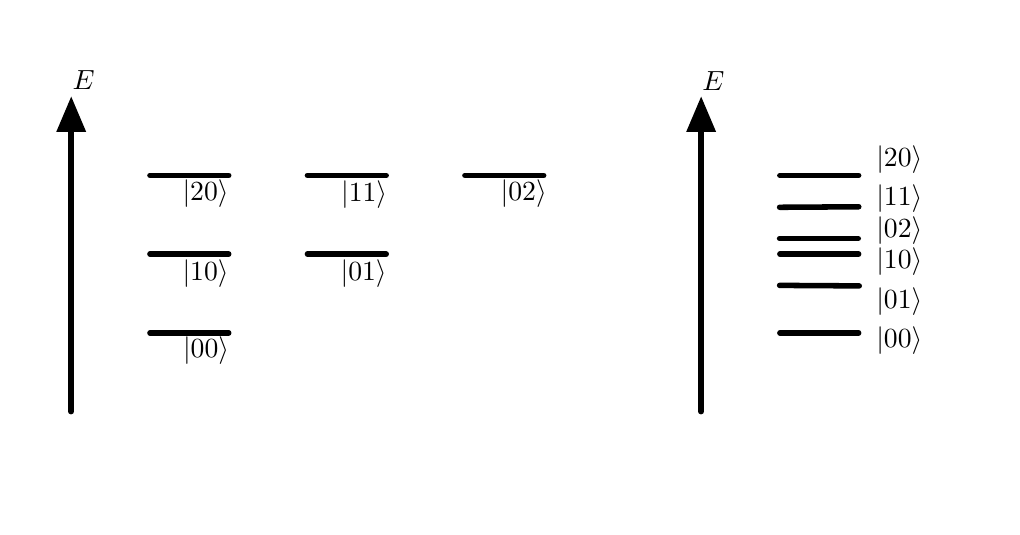
\begin{tikzpicture}[line cap=round,line join=round,>=triangle 45,x=1cm,y=1cm]
\clip(-23.553418317641174,6.795101079060523) rectangle (-11.302431212136542,12.875976052344312);
\draw [line width=2pt] (-22,11)-- (-21,11);
\draw [line width=2pt] (-22,10)-- (-21,10);
\draw [line width=2pt] (-22,9)-- (-21,9);
\draw [line width=2pt] (-20,11)-- (-19,11);
\draw [line width=2pt] (-20,10)-- (-19,10);
\draw [line width=2pt] (-18,11)-- (-17,11);
\draw [->,line width=2pt] (-23,8) -- (-23,12);
\draw (-21.711308393868624,11.072110625259079) node[anchor=north west] {$\ket{20}$};
\draw (-19.69709823500314,11.059362459696638) node[anchor=north west] {$\ket{11}$};
\draw (-17.670139910575212,11.072110625259079) node[anchor=north west] {$\ket{02}$};
\draw (-21.711308393868624,10.058631463045113) node[anchor=north west] {$\ket{10}$};
\draw (-19.70347231778436,10.058631463045113) node[anchor=north west] {$\ket{01}$};
\draw (-21.704934311087406,9.070648631956029) node[anchor=north west] {$\ket{00}$};
\draw [->,line width=2pt] (-15,8) -- (-15,12);
\draw [line width=2pt] (-14,9)-- (-13,9);
\draw [line width=2pt] (-14.00340182099748,9.602795680057659)-- (-12.992287308507025,9.596396221117846);
\draw [line width=2pt] (-14,10)-- (-13,10);
\draw [line width=2pt] (-14.00340182099748,10.594711815728674)-- (-12.99868676744684,10.601111274668488);
\draw [line width=2pt] (-14,11)-- (-13,11);
\draw [line width=2pt] (-14.00340182099748,10.197945361460269)-- (-13.005086226386652,10.197945361460269);
\draw (-12.9,9.2) node[anchor=north west] {$\ket{00}$};
\draw (-12.9,9.7) node[anchor=north west] {$\ket{01}$};
\draw (-12.9,10.2) node[anchor=north west] {$\ket{10}$};
\draw (-12.9,10.6) node[anchor=north west] {$\ket{02}$};
\draw (-12.9,11) node[anchor=north west] {$\ket{11}$};
\draw (-12.9,11.5) node[anchor=north west] {$\ket{20}$};
\draw (-23.10723252295578,12.455286588783798) node[anchor=north west] {$E$};
\draw (-15.107758632524817,12.436164340440138) node[anchor=north west] {$E$};
\end{tikzpicture}
\end{center}
\item
Define the operators
\begin{equation}
	\hat N=\hat N_x+\hat N_y\:\:\:\:\:\:\:\:\:\:\:\hat n=\hat N_x-\hat N_y
\end{equation}
With the energy eigenstates labelled by these new eigenvalues $\ket{Nn}$
\begin{equation}
	E_{Nn}=\frac{\omega_x}{2}(N+n+1)+\frac{\omega_y}{2}(N-n+1)
\end{equation}
\begin{center}
   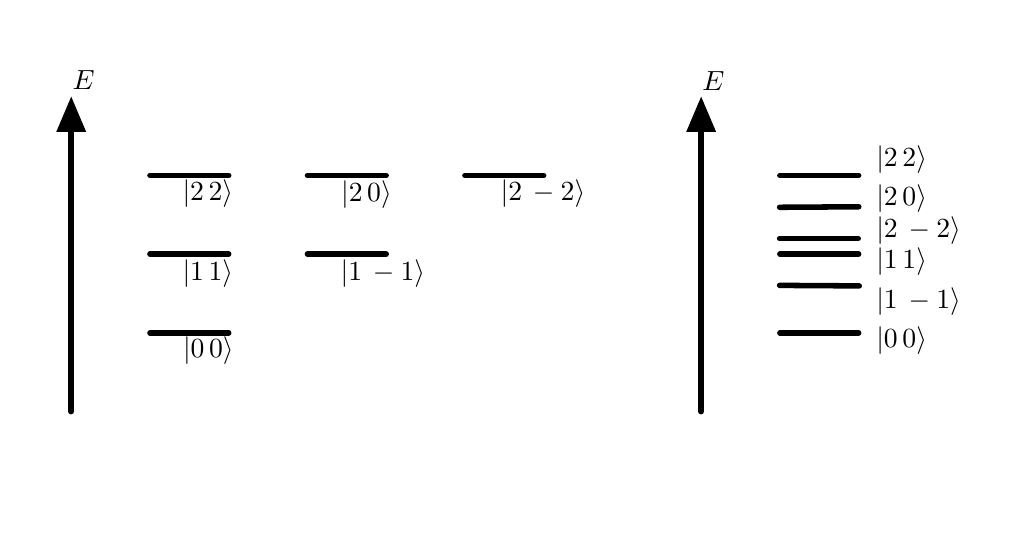
\begin{tikzpicture}[line cap=round,line join=round,>=triangle 45,x=1cm,y=1cm]
\clip(-23.553418317641174,6.795101079060523) rectangle (-11.302431212136542,12.875976052344312);
\draw [line width=2pt] (-22,11)-- (-21,11);
\draw [line width=2pt] (-22,10)-- (-21,10);
\draw [line width=2pt] (-22,9)-- (-21,9);
\draw [line width=2pt] (-20,11)-- (-19,11);
\draw [line width=2pt] (-20,10)-- (-19,10);
\draw [line width=2pt] (-18,11)-- (-17,11);
\draw [->,line width=2pt] (-23,8) -- (-23,12);
\draw (-21.711308393868624,11.072110625259079) node[anchor=north west] {$\ket{2\,2}$};
\draw (-19.69709823500314,11.059362459696638) node[anchor=north west] {$\ket{2\,0}$};
\draw (-17.670139910575212,11.072110625259079) node[anchor=north west] {$\ket{2\,-2}$};
\draw (-21.711308393868624,10.058631463045113) node[anchor=north west] {$\ket{1\,1}$};
\draw (-19.70347231778436,10.058631463045113) node[anchor=north west] {$\ket{1\,-1}$};
\draw (-21.704934311087406,9.070648631956029) node[anchor=north west] {$\ket{0\,0}$};
\draw [->,line width=2pt] (-15,8) -- (-15,12);
\draw [line width=2pt] (-14,9)-- (-13,9);
\draw [line width=2pt] (-14.00340182099748,9.602795680057659)-- (-12.992287308507025,9.596396221117846);
\draw [line width=2pt] (-14,10)-- (-13,10);
\draw [line width=2pt] (-14.00340182099748,10.594711815728674)-- (-12.99868676744684,10.601111274668488);
\draw [line width=2pt] (-14,11)-- (-13,11);
\draw [line width=2pt] (-14.00340182099748,10.197945361460269)-- (-13.005086226386652,10.197945361460269);
\draw (-12.9,9.2) node[anchor=north west] {$\ket{0\,0}$};
\draw (-12.9,9.7) node[anchor=north west] {$\ket{1\,-1}$};
\draw (-12.9,10.2) node[anchor=north west] {$\ket{1\,1}$};
\draw (-12.9,10.6) node[anchor=north west] {$\ket{2\,-2}$};
\draw (-12.9,11) node[anchor=north west] {$\ket{2\,0}$};
\draw (-12.9,11.5) node[anchor=north west] {$\ket{2\,2}$};
\draw (-23.10723252295578,12.455286588783798) node[anchor=north west] {$E$};
\draw (-15.107758632524817,12.436164340440138) node[anchor=north west] {$E$};
\end{tikzpicture}
\end{center}
If the spectrum is non-degenerate, all of the following are complete sets of commuting observables: $\{\hat N\},\{\hat N,\hat n\},\{\hat N_x,\hat N_y\}, \{\hat H\}$. However, if $\omega_x=\omega _y$, the sets $\{\hat N\}$ and $\{\hat H\}$ are no longer complete, since a distinct eigenstates can be constructed with the same eigenvalues under these operators, for example, the states $\ket{N=2,n=0}$ and $\ket{N=2,n=-2}$.\\
Similarly, if the ratio is rational: if $\omega_x/\omega_y=\alpha/\beta$, the states 
\item 
For $\omega_x=\omega_y\equiv \omega$, Evaluate the following operators
\begin{equation}
	a_x^\dagger a_y=\frac{m\omega}{2}\left(x-\frac{ip_x}{m\omega}\right)\left(y+\frac{ip_y}{m\omega}\right)=\frac{m\omega}{2}\left(xy+\frac{p_xp_y}{m^2\omega^2}\right)+\frac{i}{2}(xp_y-yp_x)
\end{equation}
\begin{equation}
	a_xa_y^\dagger=\frac{m\omega}{2}\left(x+\frac{ip_x}{m\omega}\right)\left(y-\frac{ip_y}{m\omega}\right)=\frac{m\omega}{2}\left(xy+\frac{p_xp_y}{m^2\omega^2}\right)-\frac{i}{2}(xp_y-yp_x)
\end{equation}
Therefore,
\begin{equation}
	a_x^\dagger a_y-a_xa_y^\dagger=i(xp_y-yp_x)
\end{equation}
\begin{equation}
	\hat L\equiv xp_y-yp_x=i(a_x a_y^\dagger-a_x^\dagger a_y) 
\end{equation} 
Note that for this system, the Hamiltonian is just 
\begin{equation}
	\hat H=\omega(a_x^\dagger a_x+a_y^\dagger a_y+1)
\end{equation} 
Since this system has gained rotational invariance, the angular momentum must be conserved by \textit{Noether's Theorem}. Therefore, $[\hat L,\hat H]$ must be zero.
\begin{equation}
	[\hat L,\hat H]=i\omega\left((a_x a_y^\dagger-a_x^\dagger a_y)(a_x^\dagger a_x+a_y^\dagger a_y+1)-(a_x^\dagger a_x+a_y^\dagger a_y+1)(a_x a_y^\dagger-a_x^\dagger a_y)\right)=0
\end{equation}
\item
Define the operators
\begin{equation}
	\hat a_L=\frac{1}{\sqrt{2}}(\hat a_x+ia_y),\,\,\,\,\,\,\hat a_R=\frac{1}{\sqrt{2}}(\hat a_x-i\hat a_y),\,\,\,\,\,\,\hat N_L=\hat a_L^\dagger\hat a_L,\,\,\,\,\,\,\hat N_R=\hat a_R^\dagger\hat a_R
\end{equation}
Note the following
\begin{equation}
	\hat N_L=\frac{1}{2}\left(\hat a_x^\dagger\hat a_x+\hat a_y^\dagger\hat a_y-i(\hat a_x\hat a_y^\dagger-\hat a_x^\dagger\hat a_y)\right)=\frac{1}{2}(\hat N_x+\hat N_y-\hat L)
\end{equation}
\begin{equation}
	\hat N_R=\frac{1}{2}\left(\hat a_x^\dagger\hat a_x+\hat a_y^\dagger\hat a_y+i(\hat a_x\hat a_y^\dagger-\hat a_x^\dagger\hat a_y)\right)=\frac{1}{2}(\hat N_x+\hat N_y+\hat L)
\end{equation}
The angular momentum operators can be easily re-written in terms of $\hat N_L$ and $\hat N_R$.
\begin{equation}
	\hat L=\hat N_R-\hat N_L
\end{equation} 
The Hamiltonian can also be re-written
\begin{equation}
	\hat H=\omega(\hat N_x+\hat N_y+1)=\omega(\hat N_L+\hat N_R+1)
\end{equation} 
Note that all eigenstates of the Hamiltonian are eigenstates of both $\hat N_L$ and $\hat N_R$, thus the states with their eigenvalues of these operators $\ket{LR}:\hat N_L\ket{LR}=L\ket{LR},\hat N_R\ket{LR}=R\ket{LR}$ 
The state will have the respective eigenvalues under the Hamiltonian and angular momentum operators
\begin{equation}
	\hat H\ket{LR}=\omega(L+R+1)\ket{LR}\equiv E\ket{LR}
\end{equation}
\begin{equation}
	\hat L\ket{LR}=(R-L)\ket{LR}\equiv l\ket{LR}
\end{equation} 
Because the set of operators $\{\hat N_L,\hat a_L\}$ and $\{\hat N_R,\hat a_R\}$ have the algebra of the operators $\{\hat N,\hat a\}$ for the one-dimensional simple harmonic oscillator, many of the same conclusion can be drawn. Firstly, the eigenstates of $\hat N_L$ or $\hat N_R$ are unique and orthogonal and $\hat a_L$ and $\hat a_R$ act as annihilation operators while their adjoint acts as creation operators.\\
Let an energy quantum number $n\equiv\frac{E}{\omega}-1\geq 0$. Note that $L+R=\epsilon$. Since $L$ and $R$ must take integer values and $l=R-L$
\begin{equation}
	l=2R-n\text{ for }0\leq R\leq n
\end{equation}  
Thus, for a specific energy level $n$, there are $n+1$ basis states with unique angular momentum. These states are already shown to be unique and orthogonal. Since the invariant subspace for the Hamiltonian with eigenvalue $E=\omega(n+1)$ is known to be $n+1$ dimensional, the eigenstates of angular momentum must span the entire subspace. Since this fact holds for all values of the energy, $\{\hat H,\hat L\}$ is a complete set of commuting observables for the entire Hilbert space.
\end{enumerate}
\end{sol}

\section{Problem Set 7}
\begin{sol}
\begin{enumerate}[label=\textbf{(\alph*)}]
\item 
 Since the Hamiltonian is a time-dependent Hamiltonian such that $[H(t),H(t')]=0\forall t,t'$. Thus, 
 \begin{equation}
	\mathcal U(t)=\exp\left(-i\int_0^t H(t')dt'\right)
\end{equation} 
 The potential caused by a magnetic field is 
 \begin{equation}
	H=\gamma\mathbf B\cdot\mathbf S=\gamma B_0\cos(\omega t)S_z
\end{equation} 
 \begin{equation}
	\mathcal U(t)=\exp\left(-i\gamma B_0S_z\int_0^t\cos(\omega t)dt\right)=\exp\left(-\frac{i\gamma B_0}{\omega}\sin(\omega t)S_z\right)
\end{equation} 
 \item
 \begin{equation}
	\ket{\psi,t}=\mathcal U(t)\ket{\psi,0}=\frac{1}{\sqrt{2}}\left(\exp\left(-\frac{i\gamma B_0}{\omega}\sin(\omega t)S_z\right)\ket{+}+\exp\left(-\frac{i\gamma B_0}{\omega}\sin(\omega t)S_z\right)\ket-\right)
\end{equation} 
 \begin{equation}
	=\frac{1}{\sqrt{2}}\left(\exp\left(-\frac{i\gamma B_0}{2\omega}\sin(\omega t)\right)\ket+ +\exp\left(\frac{i\gamma B_0}{2\omega}\sin(\omega t)\right)\ket-\right)
\end{equation} 
 Define a new time-dependent function \begin{equation}
	\phi(t)\equiv\frac{\gamma B_0}{\omega}\sin(\omega t)
\end{equation} 
 Rewrite the state as
 \begin{equation}
	\ket{\psi,t}=\frac{1}{\sqrt{2}}\left(e^{\frac{-i\phi}{2}}\ket++e^{\frac{i\phi}{2}}\ket-\right)
\end{equation} 
It is known that a spin in a arbitrary direction corresponding to the unit vector $\mathbf n(\theta, \phi)$ is
\begin{equation}
	\ket{\mathbf{n}}=\cos\left(\frac{\theta}{2}\right)\ket{+}+e^{i\phi}\sin\left(\frac{\theta}{2}\right)\ket{-}
\end{equation}
Re-normalizing can yield
 \begin{equation}
	\ket{\psi,t}=\frac{e^{\frac{-i\phi}{2}}}{\sqrt{2}}\left(\ket++e^{i\phi}\ket-\right)=e^{\frac{-i\phi}{2}}\left(\cos\Big(\frac{\pi}{4}\Big)\ket++\sin\Big(\frac{\pi}{4}\Big)e^{i\phi}\ket-\right)
\end{equation} 
 In this form, it is clear that $\theta(t)=\frac{\pi}{2}$ and $\phi(t)$ is exactly what's shown above.
 \item
 The probability of measuring $S_x=-\frac{1}{2}$ is
 \begin{equation}
	|\braket{-_x}{\psi,t}|^2=\Bigg|\frac{1}{2}\begin{pmatrix}
 1&-1
 \end{pmatrix}\begin{pmatrix}
 e^{\frac{-i\phi}{2}}\\e^{\frac{i\phi}{2}}
 \end{pmatrix}\Bigg|^2=\sin^2\left(\frac{\phi(t)}{2}\right)
\end{equation}
 \item
 A full flip in $S_x$ corresponds to $\phi(t)=\pi$ at some point in time. 
 \begin{equation}
	\max_{\forall t}\phi(t)=\frac{\gamma B_0}{\omega}\geq\pi\therefore\omega\leq\frac{\gamma B}{\pi}
\end{equation}
 
\end{enumerate}
\end{sol}
\begin{sol}
It has been derived that the equation for the Heisenberg operator is
\begin{equation}
	\frac{d\hat A_H}{dt}=\frac{\partial \hat A_S}{\partial t}-i[\hat A_H,\hat H_H]
\end{equation}
Since the Schrodinger operators $\hat S_x,\hat S_y,\hat S_z$ are time-independent, therefore
\begin{equation}
	\frac{d\hat A_H}{dt}=-i[\hat A_H,\hat H_H]
\end{equation}
The time evolution of Heisenberg operator for $S_z$ is trivial since it commutes with the Hamiltonian. Thus, the it is time independent and it is equal to the Schrodinger operator.\\
It is known that the commutators
\begin{equation}
	[\hat S_i,\hat S_j]=i\epsilon_{ijk}\hat S_k
\end{equation} 
Thus,
\begin{equation}
	\frac{d(\hat S_x)_H}{dt}=-i[\hat S_x,\hat H]=i\lambda B[\hat S_x,\hat S_z]=\lambda B\hat S_y
\end{equation}
\begin{equation}
	\frac{d(\hat S_y)_H}{dt}=-i[\hat S_y,\hat H]=i\lambda B[\hat S_y,\hat S_z]=-\lambda B\hat S_x
\end{equation}
Solving the differential equations with the initial conditons that $(\hat S_x)_H(0)=\hat S_x$ and $(\hat S_y)_H(0)=\hat S_y$. The Heisenberg operators can be obtained.
\begin{equation}
	(\hat S_x)_H=\hat S_x+\lambda Bt\hat S_y\:\:\:\:\:\:\:\:(\hat S_y)_H=\hat S_y-\lambda Bt\hat S_x\:\:\:\:\:\:\:\:\:(\hat S_z)_H=S_y
\end{equation} 

\end{sol}
\begin{sol}
\begin{enumerate}[label=\textbf{(\alph*)}]
\item
The Heisenberg Hamiltonian is 
\begin{equation}
	\hat H_H=\frac{\hat p_H}{2m}+V(\hat x_H)
\end{equation} 
The momentum and position operators have no explicit time-dependence. Therefore, the formula used in \textit{2, p.58} can be used. 
\begin{equation}
	\frac{d\hat p_H}{dt}=-i[\hat p_H,\hat H_H]=-i[\hat p_H,V(\hat x_H)]
\end{equation}
It is shown in \textit{1e, p.28} that $[f(x),p]=if'(x)$ 
\begin{equation}
	\frac{d\hat p_H}{dt}=-V'(x)
\end{equation}
Apply the initial conditions at $t=0$ will yield the solution
\begin{equation}
	\hat p_H=\hat p-V'(x)t
\end{equation} 
It was shown on \textit{4.b, p.50} that the commutator $[x,p^2]=2i\hat p$ 
\begin{equation}
	\frac{d\hat x_H}{dt}=-i[\hat x_H,\hat H_H]=-\frac{i}{2m}[\hat x_H,\hat p_H^2]=\frac{\hat p_H}{m}
\end{equation}
Applying the initial condition at $t=0$ will yield the solution
\begin{equation}
	\hat x_H=\hat x+\frac{\hat p_H}{m}t
\end{equation}
To compute the derivatives of the expectation values
\begin{equation}
	\frac{d}{dt}\langle \hat p\rangle=\frac{d}{dt}\bra{\psi,0}\hat p_H\ket{\psi,0}=\bra{\psi,0}\frac{d\hat p_H}{dt}\ket{\psi,0}=\bra{\psi,0}-V'(\hat x)\ket{\psi,0}=-\langle V'(\hat{x})\rangle
\end{equation} 
\begin{equation}
	\frac{d}{dt}\langle\hat x\rangle=\frac{d}{dt}\bra{\psi,0}\hat x_H\ket{\psi,0}=\bra{\psi,0}\frac{d\hat x_H}{dt}\ket{\psi,0}=\bra{\psi,0}\frac{\hat p_H}{m}\ket{\psi,0}=\frac{\langle \hat p\rangle}{m}
\end{equation} 
These results are known as \textit{Ehrenfest's theorem}. To obtain newton's second law, take the second derivative of $\langle \hat x\rangle$
\begin{equation}
	\frac{d^2}{dt^2}\langle x\rangle=\frac{d}{dt}\frac{\langle p\rangle}{m}=-\frac{\langle V'(x)\rangle}{m}
\end{equation} 
Recall a force due to a potential in classical mechanics $F=-\nabla V$. Here, define quantum mechanical force to be $\hat F\equiv-V'(\hat x)$. Also recall that the second time derivative of position is acceleration, $\hat a=\frac{d^2\hat x}{dt^2}$  (note $\hat a$ is not the annihilation operator) Rearrange the equation such that it takes a familiar form.
\begin{equation}
	\langle\hat F\rangle=m\langle\hat a\rangle
\end{equation} 
\item
The initial position and momentum of the state is known to be $x_0$ and $p_0$ respectively. Since it is a free particle, the momentum is constant. From \textit{Ehrenfest's theorem}, 
\begin{equation}
	\frac{d}{dt}\langle\hat x\rangle=\frac{p_0}{m}
\end{equation}
\begin{equation}
	\langle\hat x\rangle=x_0+\frac{p_0}{m}t
\end{equation} 
\item
The Hamiltonian for this particle in an electric field is
\begin{equation}
	\hat H=\frac{\hat p^2}{2m}+qE_0\hat x\sin(\omega t)
\end{equation}
Let $t_1$ be a time where $\sin(\omega t)$ is zero, let $t_2$ be a time where $\sin(\omega t)$ is non-zero value $\beta$.
\begin{equation}
	[\hat H(t_1),\hat H(t_2)]=\frac{\beta qE_0}{2m}[\hat p^2,\hat x]=\frac{-i\beta qE_0}{m}\hat p\neq 0
\end{equation} 
The derivation of \textit{Ehrenfest's theorem} still holds since there are no assumptions made about the nature of the Hamiltonian in the derivation. Because the unitary time-evolution operators still exist for this Hamiltonian, thus, the Heisenberg operators must also exist as $\hat A_H=\hat U_t^\dagger\hat A\hat U_t$.
\item
Using the equivalent to newton's second law, 
\begin{equation}
	\frac{d^2}{dt^2}\langle\hat x\rangle=-\frac{\langle V'(\hat x)\rangle}{m}=\frac{-qE_0\sin(\omega t)}{m}
\end{equation}
\begin{equation}
	\langle\hat x\rangle=\langle\hat x\rangle_{t=0}+\frac{1}{m}\left(\langle\hat p\rangle_{t=0}+\frac{qE_0}{\omega}\right)t+\frac{qE_0}{m\omega^2}\sin(\omega t)
\end{equation}
\end{enumerate}
\end{sol}

\begin{sol}
\begin{enumerate}[label=\textbf{(\alph*)}]
\item
Since the operator $\Omega$ has no explicit time dependence in the Schrodinger picture, the Heisenberg equation of motion is
\begin{equation}
	\frac{d\Omega_H}{dt}=-i[\hat\Omega_H,\hat H_H]=-\frac{i}{2m}[\hat{\mathbf r}_H\cdot \hat{\mathbf p}_H,\hat{\mathbf p}_H^2]-i[\hat{\mathbf r}_H\cdot \hat{\mathbf p}_H,V(\hat {\mathbf{r}}_H)]
\end{equation}  
Compute the first commutation relation by separating into components. The commutator $[\hat x\hat p,\hat p^2]$ is computed in \textit{4c, p.51} to be $2i\hat p^2$. It is also known that position and momentum along different axis commute.
\begin{equation}
	[\hat{\mathbf r}_H\cdot \hat{\mathbf p}_H,\hat{\mathbf p}_H^2]=[r_xp_x,p_x^2]+[r_yp_y,p_y^2]+[r_zp_z,p_z^2]=2i\hat{\mathbf p}_H^2
\end{equation}
The commutation relation $[\hat{\mathbf r}_H\cdot \hat{\mathbf p}_H,V(\hat {\mathbf{r}}_H)]$ is similar to that computed in \textit{4c, p.51}

\begin{equation}
	[\hat{\mathbf r}_H\cdot \hat{\mathbf p}_H,V(\hat {\mathbf{r}}_H)]=\hat{\mathbf r}_H\cdot \hat{\mathbf p}_HV(\hat {\mathbf{r}}_H)-V(\hat {\mathbf{r}}_H)\hat{\mathbf r}_H\cdot \hat{\mathbf p}_H=-i\hat{ \mathbf r}_H\cdot(\nabla( V(\hat {\mathbf{r}}_H))-V(\hat {\mathbf{r}}_H)\nabla)
\end{equation} 
Using the chain rule
\begin{equation}
	=-i\hat{ \mathbf r}_H\cdot(\nabla V(\hat {\mathbf{r}}_H)+V(\hat {\mathbf{r}}_H)\nabla-V(\hat {\mathbf{r}}_H)\nabla)=-i\hat{ \mathbf r}_H\cdot\nabla V(\hat {\mathbf{r}}_H)
\end{equation}

\begin{equation}
	\frac{d\Omega_H}{dt}=\frac{\hat{\mathbf p}_H^2}{m}-\hat {\mathbf r}_H\cdot\nabla V(\hat {\mathbf r}_H)
\end{equation} 
\item
The Heisenberg equation of motion holds for all Heisenberg operators, 
\begin{equation}
	\frac{d\hat A_H}{dt}=\frac{\partial \hat A_S}{\partial t}-i[\hat A_H,\hat H_H]
\end{equation}
If the Schrodinger operator is time-independent, the first term on the right hand side cancels. Expand the commutator to obtain
\begin{equation}
	\frac{d\hat A_H}{dt}=i(\hat H_H\hat A_H-\hat A_H\hat H_H)
\end{equation} 
Take the expectation value of this operator on any stationary state $\ket{\Psi,0}$ with a energy eigenvalue $E$.
\begin{equation}
	\left\langle\frac{d\hat A_H}{dt}\right\rangle=i(\bra{\Psi,0}\hat H_H\hat A_H\ket{\Psi,0}-\bra{\Psi,0}\hat A_H\hat H_H\ket{\Psi,0})
\end{equation}\begin{equation}
	=i(E\bra{\Psi,0}\hat A_H\ket{\Psi,0}-E\bra{\Psi,0}\hat A_H\ket{\Psi,0})=0
\end{equation}
\item
For a stationary state of the Hamiltonian, the operator $\Omega$ must be time independent. This states that
\begin{equation}
	\frac{d\Omega_H}{dt}=\frac{\hat{\mathbf p}_H^2}{m}-\hat {\mathbf r}_H\cdot\nabla V(\hat {\mathbf r}_H)=0
\end{equation} 
\begin{equation}
	\therefore\frac{\hat{\mathbf p}_H^2}{m}=\hat {\mathbf r}_H\cdot\nabla V(\hat {\mathbf r}_H)
\end{equation}
In spherical coordinates
\begin{equation}
	\nabla V=\frac{\partial V}{\partial r}\hat r+\frac{1}{r\sin\phi}\frac{\partial V}{\partial\theta}\hat\theta+\frac{1}{r}\frac{\partial V}{\partial\phi}\hat\phi
\end{equation}
Since a central potential is angularly independent, the gradient reduces to the first term. Similarly, the dot product reduces to a ordinary scalar product. For the potential $V(r)=c/r^k$,
\begin{equation}
	\frac{\hat{\mathbf p}_H^2}{m}=r\frac{\partial V}{\partial r}=-r\frac{kc}{r^{k+1}}=-\frac{kc}{r^k}=-kV(r)
\end{equation}  
Since the kinetic energy is equal to $\frac{\hat{\mathbf p}_H^2}{2m}$. Multiplying both sides by 2 and taking the expectation value yields
\begin{equation}
	\langle T\rangle=-\frac{k}{2}\langle V\rangle
\end{equation}

\end{enumerate}
\end{sol}
\newpage
\begin{sol}
\begin{enumerate}[label=\textbf{(\alph*)}]
\item
Since the position and momentum operators have no explicit time-dependence, the Heisenberg equations of motion are
$$\frac{d\hat x_H}{dt}=-i[\hat x_H,\hat H_H]=-\frac{i}{2m}[\hat x_H,\hat p_H^2]=\frac{\hat p_H}{m}$$
$$\frac{d\hat p_H}{dt}=-i[\hat p_H,\hat H_H]=-ig[p_H, x_H]=-g$$
Applying the initial conditions will yield
$$\hat x_H(t)=\hat x+\int_0^t\frac{\hat p_H(t')}{m}dt'=\hat x+\frac{1}{m}\left(\hat pt-\frac{gt^2}{2}\right)$$
$$\hat p_H(t)=\hat p-gt$$ 
\item
$$\bra\psi\hat x_H(t)\ket\psi=\bra\psi\hat x\ket\psi+\frac{1}{m}(\bra\psi\hat p\ket\psi t-gt^2\braket{\psi}{\psi})=0-\frac{1}{m}\left(0-\frac{gt^2}{2}\right)=-\frac{gt^2}{2m}$$
A classical particle starting at rest and $x=0$ that experience a constant force $-g$ will have an acceleration of $-\frac{g}{m}$. The equation of motion of a classical particle is  $x(t)=x_0+v_0t+\frac{1}{2}at^2$. With these conditions, $x(t)=-\frac{gt^2}{2m}$ which is exactly the same as the equation for $\bra\psi\hat x_H(t)\ket\psi$.
\item
Find the Heisenberg operator $\hat x_H^2=\hat x_H\hat x_H$
$$\hat x_H^2=\left(\hat x+\frac{\hat pt}{m}-\frac{gt^2}{2m}\right)\left(\hat x+\frac{\hat pt}{m}-\frac{gt^2}{2m}\right)$$ 
$$=\hat x^2+\frac{\hat x\hat pt}{m}-\frac{\hat xgt^2}{2m}+\frac{\hat p\hat xt}{m}+\frac{\hat p^2t^2}{m^2}-\frac{\hat pgt^3}{2m^2}-\frac{\hat xgt^2}{2m}-\frac{\hat pgt^3}{2m^2}+\frac{g^2t^4}{4m^2}$$ 
$$=\hat x^2+\{\hat x,\hat p\}\frac{t}{m}+\frac{\hat p^2t^2}{m^2}+\alpha\hat x+\beta\hat p$$
Compute the expectation value on a Gaussian wave-packet $\braket{x}{\psi}=\psi(x)=N\exp\left(-\frac{x^2}{2a^2}\right)$ 
$$\langle\hat x^2\rangle(t)=\bra\psi\hat x^2\ket\psi+\bra\psi\{\hat x,\hat p\}\ket\psi\frac{t}{m}+\bra\psi\hat p^2\ket\psi\frac{t^2}{m^2}+\frac{g^2t^4}{4m^2}\braket{\psi}{\psi}+\bra\psi\hat x\ket\psi\alpha+\bra\psi\hat p\ket\psi\beta$$ 
$$=\int_{-\infty}^\infty x^2\psi(x)^2dx+\frac{it}{m}\int_{-\infty}^\infty x\psi(x)\psi'(x)dx+\frac{it}{m}\int_{-\infty}^\infty\psi(x)(\psi(x)+x\psi'(x))dx$$
$$-\frac{t^2}{m^2}\int_{-\infty}^\infty\psi(x)\psi''(x)dx+\frac{g^2t^4}{4m^2}+0+0$$
$$=\frac{a^2}{2}-\frac{it}{2m}+\frac{it}{2m}+\frac{t^2}{2a^2m^2}+\frac{g^2t^4}{4m^2}=\frac{a^2}{2}+\frac{t^2}{2a^2m^2}+\frac{g^2t^4}{4m^2}$$ 
It is computed in \textit{(b)} that $\displaystyle{\langle\hat x\rangle=-\frac{gt^2}{4m}}$; therefore,
$$(\Delta x)^2=\langle\hat x^2\rangle-\langle\hat x\rangle^2=\frac{a^2}{2}+\frac{t^2}{2a^2m^2}$$
For a Gaussian wave-packet, it is known that the square of position uncertainty at $t=0$ is $\frac{a^2}{2}$. The expression can be rewritten, defining $\lambda\equiv\frac{1}{2a^2m^2}$
$$(\Delta x(t))^2=(\Delta x(0))^2+\lambda t^2$$
It has been shown that the dispersion of the wave-packet is independent of the value of $g$.

\end{enumerate}
\end{sol}
\begin{sol}
\begin{enumerate}[label=\textbf{(\alph*)}]
\item
The Hamiltonian of the shifted harmonic oscillator is 
\begin{equation}
	\hat H=\frac{\hat p^2}{2m}+\frac{1}{2}m\omega^2\hat x^2-F\hat x
\end{equation}
Complete the square for the second and third terms of the Hamiltonian. Let a characteristic length $\beta\equiv\frac{F}{m\omega^2}$
\begin{equation}
	\hat H=\frac{p^2}{2m}+\frac{1}{2}m\omega^2(\hat x-\beta)^2-\frac{1}{2}m\omega^2\beta^2
\end{equation}
Define a new position operator $\hat y\equiv \hat x-\beta$. The Hamiltonian can be rewritten as
\begin{equation}
	\hat H=\frac{p^2}{2m}+\frac{1}{2}m\omega^2\hat y^2-\frac{1}{2}m\omega^2\beta^2
\end{equation}
It is clear that this Hamiltonian is analogous to the Hamiltonian of the normal simple harmonic oscillator with $\hat y$ being the position operator. For a simple harmonic oscillator, the expectation value of the position in the ground state is zero. Thus, $\langle\hat y\rangle=0$. 
\begin{equation}
	\langle x\rangle=\langle y\rangle-\beta=-\frac{F}{m\omega^2}
\end{equation}
\item
Define the operator
\begin{equation}
	\hat a_y\equiv\sqrt{\frac{m\omega}{2}}\left(\hat y+\frac{i\hat p}{m\omega}\right)=\hat a-\sqrt{\frac{m\omega}{2}}\beta
\end{equation}
This is the annihilation operator of the shifted harmonic oscillator. Thus, $\hat a_y\ket {0'}=0$.
It is given that 
\begin{equation}
	\ket{0'}=Ne^{\alpha \hat a^\dagger}\ket 0
\end{equation}
For simplicity, let $\gamma\equiv\sqrt{\frac{m\omega}{2}}\beta$ 
\begin{equation}
	\hat a_y\ket{0'}=(\hat a-\gamma)Ne^{\alpha \hat a^\dagger}\ket 0=0
\end{equation} 
Since $N$ is a constant, it can be ignored. Rearranging the terms will result in
\begin{equation}
	\hat ae^{\alpha\hat a^\dagger}\ket 0=\gamma e^{\alpha\hat a^\dagger}\ket 0
\end{equation}
Note that $[\hat a,e^{\alpha\hat a^\dagger}]\ket 0=\hat ae^{\alpha\hat a^\dagger}\ket 0+e^{\alpha\hat a^\dagger}\hat a\ket 0=\hat ae^{\alpha\hat a^\dagger}\ket 0$. Hence, $[\hat a,e^{\alpha\hat a^\dagger}]\ket 0=\gamma e^{\alpha\hat a^\dagger}\ket 0$.\\
It will be helpful to compute the commutator. First, use the definition of the exponential and the linearity of the commutator.
\begin{equation}
	[\hat a,e^{\alpha\hat a^\dagger}]=\sum_{n=0}^\infty\frac{\alpha^n}{n!}[a,(a^\dagger)^n]
\end{equation}
It was computed in \textit{5b, p.52} that $[a,(a^\dagger)^n]=n(a^\dagger)^{n-1}$ for $n\geq 1$. Note that $a$ commutes with $(a^\dagger)^0$ which is the identity operator.
\begin{equation}
	[\hat a,e^{\alpha\hat a^\dagger}]=\sum_{n=1}^\infty\frac{\alpha^n}{n!}[a,(a^\dagger)^n]=\sum_{n=1}^\infty\frac{\alpha^n}{n!}n(a^\dagger)^{n-1}=\sum_{n=1}^\infty\frac{\alpha^n(a^\dagger)^{n-1}}{(n-1)!}=\alpha\sum_{j=0}^\infty\frac{\alpha^j(a^\dagger)^{j}}{j!}=\alpha e^{\alpha \hat a^\dagger}
\end{equation} 
Substituting this result in the previous expression will yield
\begin{equation}
	[\hat a,e^{\alpha\hat a^\dagger}]\ket 0=\alpha e^{\alpha\hat a^\dagger}\ket 0=\gamma e^{\alpha\hat a^\dagger}\ket 0
\end{equation}
\begin{equation}
	\alpha=\gamma=\sqrt{\frac{m\omega}{2}}\frac{F}{m\omega^2}=\frac{F}{\sqrt{2m\omega^3}}
\end{equation} 

\end{enumerate}
\end{sol}
\begin{sol}
Rewrite the unitary operator $e^{\alpha\hat a^\dagger-\alpha^*\hat a}$ in terms of the position and momentum operators. From the definition of the creation and annihilation operators,
\begin{equation}
	e^{\alpha\hat a^\dagger-\alpha^*\hat a}=\exp\left(\sqrt{\frac{m\omega}{2}}\left(\alpha\hat x-\frac{i\alpha\hat p}{m\omega}-\alpha^*\hat x-\frac{i\alpha^*\hat p}{m\omega}\right)\right)=\exp\left(i\sqrt{2m\omega}\left(\text{Im}(\alpha)\hat x-\frac{\text{Re}(\alpha)\hat p}{m\omega}\right)\right)
\end{equation}
Note this operator takes a similar form to the position and momentum translation operators. Let $x_0\equiv\sqrt{\frac{2}{m\omega}}\text{Re}(\alpha)$ and $p_0=\sqrt{2m\omega}\text{Im}(\alpha)$, the operator can be rewritten as
\begin{equation}
	e^{\alpha\hat a^\dagger-\alpha^*\hat a}=\exp(ip_0\hat x-i\hat px_0)
\end{equation}
Using the \textit{Baker-Campbell-Hausdorff Theorem}, 
\begin{equation}
	\exp(ip_0\hat x-i\hat px_0)=e^{ip_0\hat x}e^{-i\hat px_0}e^{-\frac{1}{2}[ip_0\hat x,-ix_0\hat p]}=T_{x_0}\tilde {T}_{p_0}e^{-\frac{1}{2}[ip_0\hat x,-ix_0\hat p]}
\end{equation} 
The commutator has been computed on \textit{1b, p.37} to be $-ix_0p_0\mathbf{1}$. Thus, the exponentiation of the commutator will just be a pure phase.\\
The coherent states are defined to be
\begin{equation}
	\ket\alpha=e^{\alpha\hat a^\dagger-\alpha^*\hat a}\ket 0=e^{-\frac{1}{2}ix_0p_0}T_{x_0}\tilde {T}_{p_0}\ket 0
\end{equation} 
\begin{equation}
	\braket{x}{0}=\frac{1}{\sqrt{a\sqrt{\pi}}}e^{-\frac{x^2}{2a^2}}
\end{equation}
Acting with the position and momentum translation operators will yield
\begin{equation}
	\braket{x}{\alpha}=e^{-\frac{1}{2}ix_0p_0}\bra xT_{x_0}\tilde {T}_{p_0}\ket 0=e^{ip_0x}\braket{x-x_0}{0}=\frac{e^{-\frac{1}{2}ix_0p_0}}{\sqrt{a\sqrt{\pi}}}e^{ipx}e^{-\frac{(x-x_0)^2}{2a^2}}
\end{equation} 
This is indeed a Gaussian function that is normalized as $\braket{\alpha}{\alpha}=1$.
\end{sol}
\newpage
\section{Problem Set 8}
\begin{sol}
\begin{lemma}
$$[[A,B],B]=0\implies[A,e^B]=[A,B]e^B$$
\end{lemma}
\begin{proof}
Multiply $[A,e^B]$ by the identity operator $\mathbf 1=e^{-B}e^B$ on the right to obtain
$$[A,e^B]=[A,e^B]e^{-B}e^B=Ae^B-e^BAe^{-B}e^B=(A-e^BAe^{-B})e^B$$ 
The \textit{Hadamard Lemma (p.30)} to $e^BAe^{-B}$ taking into consideration the hypothesis that $[[A,B],B]=0$ can be used to simplify this term to $A-[B,A]$. Because $-[B,A]=[A,B]$, 
$$[A,e^B]=(A-A+[A,B])e^B=[A,B]e^B$$


\end{proof}
\begin{enumerate}[label=\textbf{(\alph*)}]
    \item 
    The position eigenstates of the harmonic oscillator is constructed by taking the limit as the squeezing parameter approaches infinity. 
    $$S_\gamma = \exp\left(-\frac{\gamma}{2}(\hat a^\dagger\hat a^\dagger-\hat a\hat a)\right)=\frac{1}{\sqrt{\cosh\gamma}}\exp\left(-\frac{1}{2}\tanh\gamma\hat a^\dagger\hat a^\dagger\right)$$
    $$S_\infty=e^{-\frac{1}{2}\hat a^\dagger\hat a^\dagger}$$
    A state proportional to $S_\infty\ket 0$ will be annihilated by the position operator.\\
    The position translation operator can be written using \textit{Baker-Campbell-Hausdorff Theorem} as
    $$T_y = e^{y(\hat a^\dagger-\hat a)}=e^{y\hat a^\dagger}e^{-y\hat a}e^{-\frac{y}{2}[\hat a, \hat a^\dagger]}=e^{-\frac{y^2}{2}}e^{y\hat a^\dagger}e^{-y\hat a}$$ 
    Where $y$ is the dimensionless position quantity $y= x\sqrt{2m\omega}$. The operator $e^{-y\hat a}$ can be expanded into its polynomial, which acting on the vacuum state will be equivalent to the identity operator. Thus, up to a normalization constant
    $$T_y\ket 0=e^{-\frac{y^2}{2}}e^{y\hat a^\dagger}\ket 0$$
    The general position eigenstate will be
    $$\ket y = e^{-\frac{y^2}{2}}\exp\left(y\hat a^\dagger-\frac{1}{2}\hat a^\dagger\hat a^\dagger\right)\ket 0$$
    The bra will then be 
    $$\bra y =  e^{-\frac{y^2}{2}}\bra 0\exp\left(y\hat a^\dagger-\frac{1}{2}\hat a^\dagger\hat a^\dagger\right)$$ $$\braket{y}{2}=\frac{1}{\sqrt 2}e^{-\frac{y^2}{2}}\bra 0\exp\left(y\hat a-\frac{1}{2}\hat a\hat a\right)\hat a^\dagger\hat a^\dagger\ket 0$$
    The creation operators will annihilate the bra. They can be commuted to the left by using the commutation relations. The commutators can be evaluated with Lemma 12.
    $$\exp\left(y\hat a-\frac{1}{2}\hat a\hat a\right)a^\dagger =a^\dagger\exp\left(y\hat a-\frac{1}{2}\hat a\hat a\right)+\left[\exp\left(y\hat a-\frac{1}{2}\hat a\hat a\right),\hat a^\dagger\right]$$ $$\left[\exp\left(y\hat a-\frac{1}{2}\hat a\hat a\right),\hat a^\dagger\right]=\exp\left(y\hat a-\frac{1}{2}\hat a\hat a\right)\left[y\hat a-\frac{1}{2}\hat a\hat a,\hat a^\dagger\right]$$
    $$=\exp\left(y\hat a-\frac{1}{2}\hat a\hat a\right)\left(y[\hat a, \hat a^\dagger]-\frac{1}{2}[\hat a\hat a,\hat a^\dagger] \right)=\exp\left(y\hat a-\frac{1}{2}\hat a\hat a\right)(y-\hat a)$$ 
Then,
$$\exp\left(y\hat a-\frac{1}{2}\hat a\hat a\right)a^\dagger=a^\dagger\exp\left(y\hat a-\frac{1}{2}\hat a\hat a\right)+\exp\left(y\hat a-\frac{1}{2}\hat a\hat a\right)(y-\hat a)$$
    With this, the wave-function of $\ket 2$ can be rewritten as three terms by bring one of the creation operators to the left of the exponential.
    $$\braket{y}{2}=\frac{1}{\sqrt{2}}e^{-\frac{y^2}{2}}\left(-\bra 0a^\dagger e^{y\hat a-\frac{1}{2}\hat a\hat a}a^\dagger\ket 0+y\bra 0e^{y\hat a-\frac{1}{2}\hat a\hat a}a^\dagger\ket 0-\bra 0e^{y\hat a-\frac{1}{2}\hat a\hat a}\hat a\hat a^\dagger\ket 0\right)$$ 
    The first term evaluates to zero. The second term can be evaluated by commuting the creation and annihilation operators with $\hat a\hat a^\dagger = \hat a^\dagger \hat a+[\hat a, \hat a^\dagger]=\hat a^\dagger \hat a+1$. The third term can be expanded with the relation derived above.
    $$\frac{1}{\sqrt 2}e^{-\frac{y^2}{2}}\left(y\bra 0a^\dagger e^{y\hat a-\frac{1}{2}\hat a\hat a}\ket 0-y\bra 0e^{y\hat a-\frac{1}{2}\hat a\hat a}\hat a\ket0+y^2\bra 0e^{y\hat a-\frac{1}{2}\hat a\hat a}\ket0-\bra 0e^{y\hat a-\frac{1}{2}\hat a\hat a}(a^\dagger a+1)\ket 0\right)$$
    The first two terms evaluate to zero. In the final term, $\hat a^\dagger a+1$ acts like the identity on the ground state, thus, the wave function will take the form
    $$\braket{y}{2}=\frac{1}{\sqrt 2}e^{-\frac{y^2}{2}}(y^2-1)\bra 0e^{y\hat a-\frac{1}{2}\hat a\hat a}\ket 0$$
    \item
    The momentum eigenstates can be constructed by a momentum translation of the zero momentum eigenstate, which is given by taking the limit as the squeezing parameter approaches negative infinity. 
    $$\ket{p=0}=S_{-\infty}\ket 0=e^{\frac{1}{2}\hat a^\dagger\hat a^\dagger}\ket 0$$
    The momentum translation operator is
    $$T_q = e^{iq(\hat a+\hat a^\dagger)}$$
    Where $p$ is the dimensionless momentum quantity $q=\frac{p\sqrt{2}}{\sqrt{m\omega}}$. Using the \textit{Baker-Campbell-Hausdorff Theorem}, 
    $$T_q = e^{iq\hat a^\dagger}e^{iq\hat a}e^{\frac{iq}{2}[\hat a,\hat a^\dagger]}=e^{\frac{iq}{2}}e^{iq\hat a^\dagger}e^{iq\hat a}$$
    The operator $e^{iq\hat a}$ can be expanded into its polynomial, which acting on the vacuum state will the equivalent to the identity operator. Thus, up to a phase
    $$T_q\ket 0 = e^{iqa^\dagger}\ket 0$$
    The general momentum eigenstates $\ket q$ can be constructed by
    $$\ket q = S_{-\infty}T_q\ket 0=\exp\left(iq\hat a^\dagger+\frac{1}{2}a^\dagger a^\dagger\right)\ket0=e^{\frac{1}{2}\hat a^\dagger\hat a^\dagger}e^{iqa^\dagger}\ket 0=e^{iqa^\dagger}e^{\frac{1}{2}\hat a^\dagger\hat a^\dagger}\ket{0}$$
    This state is a eigenstate of the momentum operator. Let the dimensionless momentum operator be $\hat q = i(a^\dagger-a)$. The commutator can be evaluated with Lemma 12
    $$\hat q\ket q=ia^\dagger \ket q-ia\ket q=ia^\dagger \ket q-i\left[a, \exp\left(iq\hat a^\dagger+\frac{1}{2}a^\dagger a^\dagger\right)\right]\ket 0$$
    $$=ia^\dagger \ket q-i\left[a, iq\hat a^\dagger+\frac{1}{2}a^\dagger a^\dagger\right]\exp\left(iq\hat a^\dagger+\frac{1}{2}a^\dagger a^\dagger\right)\ket 0$$
    The commutator can be written as
    $$\left[a, iq\hat a^\dagger+\frac{1}{2}a^\dagger a^\dagger\right]=iq[a,\hat a^\dagger]+\frac{1}{2}[a, (a^\dagger)^2]$$
    From \textit{5b, p.52}, it has been shown that $[a, (a^\dagger)^2]=2a^\dagger$. Also, note that $\exp\left(iq\hat a^\dagger+\frac{1}{2}a^\dagger a^\dagger\right)\ket 0=\ket q$. 
    $$\hat q\ket q=ia^\dagger \ket q+q\ket q-ia^\dagger \ket q=q\ket q$$
   	$\because q=\frac{p\sqrt{2}}{\sqrt{m\omega}}$ and $\hat q = \frac{p\sqrt{2}}{\sqrt{m\omega}}$, $\hat q\ket q=q\ket q\iff\hat p\ket p=p\ket p$
\end{enumerate}
\end{sol}
\begin{sol}
The coherent state $\ket\alpha$ is defined to be $e^{\alpha\hat a^\dagger-\alpha^*\hat a}\ket0$.
\begin{enumerate}[label=\textbf{(\alph*)}]
\item
$$\hat a\ket\alpha=\hat ae^{\alpha\hat a^\dagger-\alpha^*\hat a}\ket0=[\hat a, e^{\alpha\hat a^\dagger-\alpha^*\hat a}]\ket 0=[\hat a, \alpha\hat a^\dagger-\alpha^*\hat a]e^{\alpha\hat a^\dagger-\alpha^*\hat a}\ket0=\alpha[a,a^\dagger]\ket\alpha=\alpha\ket\alpha$$ 
\item
Using the \textit{Baker-Campbell-Hausdorff Theorem},
$$e^{\alpha\hat a^\dagger-\alpha^*\hat a}=e^{\alpha\hat a^\dagger}e^{-\alpha^*\hat a}e^{-\frac{|\alpha|^2}{2}[\hat a, \hat a^\dagger]}=e^{-\frac{|\alpha|^2}{2}}e^{\alpha\hat a^\dagger}e^{-\alpha^*\hat a}$$
Acting on the vacuum state, $e^{-\alpha^*\hat a}$ will behave like the identity operator. 
$$\ket\alpha=e^{-\frac{|\alpha|^2}{2}}e^{\alpha\hat a^\dagger}\ket0$$
The exponential can be expanded with its series definition
$$\ket\alpha=e^{-\frac{|\alpha|^2}{2}}\sum_{n=0}^\infty \frac{\alpha^n }{n!}(a^\dagger)^n\ket 0$$ 
It is known that $(a^\dagger)^n\ket 0=\sqrt{n!}\ket n$ 
$$\ket\alpha=e^{-\frac{|\alpha|^2}{2}}\sum_{n=0}^\infty \frac{\alpha^n }{\sqrt{n!}}\ket n$$ 
The probability amplitude of each energy eigenstate is $e^{-\frac{|\alpha|^2}{2}}\frac{\alpha^n }{\sqrt{n!}}$. The norm squared is the probability. Defining $\lambda=|\alpha|^2$,
$$|\braket{n}{\alpha}|^2=\frac{e^{-\lambda}\lambda^n}{n!}$$
\item
The inner product can be done in the energy basis. The bra is
$$\bra\beta=e^{-\frac{|\beta|^2}{2}}\sum_{n=0}^\infty\frac{(\beta^*)^n}{\sqrt{n!}}\bra n$$  
Since the energy basis is orthonormal, the inner product can be simplified to
$$\braket{\beta}{\alpha}=e^{-\frac{|\alpha|^2+|\beta|^2}{2}}\sum_{n=0}^\infty\frac{(\beta^*\alpha)^n}{n!}=\exp\left(\beta^*\alpha-\frac{|\alpha|^2+|\beta|^2}{2}\right)$$ As $\beta$ and $\alpha$ are finite complex numbers, the argument in the exponential is also finite, thus, the inner product cannot be zero.
\item
Evaluate the expectation value of the energy and its square
$$\bra\alpha\hat H\ket\alpha=e^{-\lambda}\sum_{n=0}^\infty\omega\left(n+\frac{1}{2}\right)\frac{\lambda^n}{n!}=\frac{\omega}{2}e^{-\lambda}\sum_{n=0}^\infty\frac{\lambda^n}{n!}+e^{-\lambda}\omega\lambda\frac{d}{d\lambda}\sum_{n=0}^\infty\frac{\lambda^n}{n!}=\omega\left(\lambda+\frac{1}{2}\right)$$
$$\bra\alpha\hat H^2\ket\alpha=e^{-\lambda}\sum_{n=0}^\infty\omega^2\left(n+\frac{1}{2}\right)^2\frac{\lambda^n}{n!}=e^{-\lambda}\sum_{n=0}^\infty\omega^2\left(n^2+n+\frac{1}{4}\right)\frac{\lambda^n}{n!}$$ 
$$=\omega^2e^{-\lambda}\left(\lambda^2\frac{d^2}{d\lambda^2}\sum_{n=0}^\infty\frac{\lambda^n}{n!}+2\lambda\frac{d}{d\lambda}\sum_{n=0}^\infty\frac{\lambda^n}{n!}+\frac{1}{4}\sum_{n=0}^\infty\frac{\lambda^n}{n!}\right)=\omega^2\left(\lambda^2+2\lambda+\frac{1}{4}\right)$$
The uncertainty is given by $\Delta E = \sqrt{\langle E^2\rangle+\langle E\rangle^2}=\omega\sqrt{\lambda^2+2\lambda+\frac{1}{4}-\left(\lambda+\frac{1}{2}\right)^2}=\omega\sqrt\lambda$. Thus,
$$\frac{\Delta E}{\langle E\rangle}=\frac{\sqrt{\lambda}}{\lambda+\frac{1}{2}}=\frac{|\alpha|}{|\alpha|^2+\frac{1}{2}}$$ 
This ratio clearly decreases as $|\alpha|$ increases. It is also asymptotically equivalent to $|\alpha|^{-1}$.
\item
Define dimensionless position and momentum $y=x\sqrt{m\omega}$ and $q=\frac{p}{\sqrt{m\omega}}$ so $[y,q]=[x,p]=i\mathbf{1}$ 
$$\bra\alpha\hat y\ket\alpha=\frac{1}{\sqrt{2}}\bra\alpha(a+a^\dagger)\ket\alpha=\frac{1}{\sqrt{2}}(\alpha+\alpha^*)\braket{\alpha}{\alpha}=\sqrt{2}\text{Re}(\alpha)$$ 
$$\bra \alpha\hat q\ket \alpha=\frac{i}{\sqrt{2}}\bra\alpha(a^\dagger-a)\ket\alpha=\frac{-1}{\sqrt{2}i}(\alpha^*-\alpha)\braket{\alpha}{\alpha}=\sqrt{2}\text{Im}(\alpha)$$
The expectation value of the square of the operator must be computed to find the uncertainties.
$$\bra\alpha\hat y^2\ket\alpha=\frac{1}{2}\bra\alpha(a+a^\dagger)^2\ket\alpha=\frac{1}{2}\left(\bra\alpha a^2\ket\alpha+\bra\alpha (a^\dagger)^2\ket\alpha+\bra\alpha a^\dagger a\ket\alpha+\bra\alpha aa^\dagger\ket\alpha\right)$$
The computation is straightforward as the bras and kets are eigenstates of the creation and annihilation operators respectively. For the final term, the commutation relation $[\hat a,\hat a^\dagger]=1$ can be used.
$$\bra\alpha\hat y^2\ket\alpha=\frac{1}{2}(\alpha^2+(\alpha^*)^2+2\alpha^*\alpha+1)=2\text{Re}(\alpha)^2+\frac{1}{2}$$ 
 $$\Delta y=\sqrt{\langle y^2\rangle-\langle y\rangle^2}=\frac{1}{\sqrt{2}}$$
 The momentum uncertainty can be calculated in a similar manner.
$$\bra\alpha\hat q^2\ket\alpha = -\frac{1}{2}\bra\alpha(a^\dagger-a)^2\ket\alpha=-\frac{1}{2}\left(\bra\alpha a^2\ket\alpha+\bra\alpha (a^\dagger)^2\ket\alpha-\bra\alpha a^\dagger a\ket\alpha-\bra\alpha aa^\dagger\ket\alpha\right)$$
$$=-\frac{1}{2}(\alpha^2+(\alpha^*)^2-2\alpha^*\alpha-1)=2\text{Im}(\alpha)^2+\frac{1}{2}$$
 $$\Delta q=\sqrt{\langle q^2\rangle-\langle q\rangle^2}=\frac{1}{\sqrt{2}}$$
It can be seen that the uncertainty relation is saturated as $\Delta y\Delta q=\Delta x\Delta p=\frac{1}{2}$
\item
The coherent state expressed in the energy basis is
$$\ket\alpha=e^{-\frac{|\alpha|^2}{2}}\sum_{n=0}^\infty \frac{\alpha^n }{\sqrt{n!}}\ket n$$
Time evolution in the energy basis is revolution by an overall phase
$$\ket{\alpha,t}=e^{-\frac{|\alpha|^2}{2}}\sum_{n=0}^\infty \frac{\alpha^ne^{-i\omega(n+\frac{1}{2} )t}}{\sqrt{n!}}\ket n=e^{-\frac{|\alpha|^2}{2}}e^{-\frac{1}{2}i\omega t}\sum_{n=0}^\infty \frac{\alpha^ne^{-i\omega nt}}{\sqrt{n!}}\ket n
$$$$=e^{-\frac{|\alpha|^2}{2}}e^{-\frac{1}{2}i\omega t}\sum_{n=0}^\infty \frac{(\alpha e^{-i\omega t})^n}{\sqrt{n!}}\ket n$$ 
Let the function $\alpha(t)=\alpha e^{-i\omega t}$. The time evolution of the coherent state $\ket\alpha$ will be $\ket{\alpha(t)}$ to a phase.
\item
Since it is computed above that the time evolution of a coherent state $\ket\alpha_0$ is $\ket{\beta(t)}$ where $\beta(t)=\alpha_0e^{-i\omega t}$, the previous computations of the expectation values for any coherent state $\ket\alpha$ can be used.
$$\langle\hat y\rangle=\sqrt{2}\text{Re}(\beta(t))=\sqrt{2}\alpha_0\cos(\omega t)\:\:\:\:\:\:\:\:\:\:\:\:\langle\hat q\rangle=\sqrt{2}\text{Im}(\beta(t))=-\sqrt{2}\alpha_0\sin(\omega t)\:\:\:\:\:\:\:\:\:\:\:\:\langle E\rangle = \omega\left(\alpha_0^2+\frac{1}{2}\right)$$
$$\Delta y = \Delta q = \frac{1}{\sqrt 2}$$
Note that energy is conserved and the position-momentum uncertainty bound remains saturated for all time.
\end{enumerate}
\end{sol}
\begin{sol}
\begin{enumerate}[label=\textbf{(\alph*)}]
\item
The operator $a(\gamma)$ is in the form $e^ABe^{-A}$, with $A=\frac{\gamma}{2}(a^\dagger a^\dagger-aa)$ and $B=a$. First, compute some commutators.
$$[A,a]=\frac{\gamma}{2}[(a^\dagger)^2,a]=-\gamma a^\dagger\:\:\:\:\:\:\:\:\:\:\:\:\:\:\:[A,[A,a]]=[A,-\gamma a^\dagger]=\gamma^2a$$ 
$$[A, a^\dagger]=\frac{\gamma}{2}[a^2, a^\dagger]=-\gamma a\:\:\:\:\:\:\:\:\:\:\:\:\:\:\:[A,[A,a^\dagger]]=[A,-\gamma a]=\gamma^2a^\dagger$$ 
Next, apply the \textit{Hadamard Lemma} proven on \textit{p.30}. Firstly, the construct the infinite sequence $W_n$. $W_0$ is defined to be $a$ and $W_1$ is computed above to be $\gamma a^\dagger$. From what is computed above, it can also be concluded that $W_{n+2}=\gamma^2W_n$. By induction, the entire sequence can be constructed as $W_{2n}=\gamma^{2n}a\text{  and  }W_{2n+1}=-\gamma^{2n+1}a^\dagger$ for all non-negative integers $n$. The \textit{Hadamard Lemma} states that 
$$e^ABe^{-A}=\sum_{n=0}^\infty\frac{W_n}{n!}$$ 
The left hand side is the operator of interest, $a(\gamma)$, whereas the right hand side can be split up into two terms.
$$a(\gamma)=\sum_{n=0}^\infty\frac{W_{2n}}{(2n)!}+\sum_{n=0}^\infty\frac{W_{2n+1}}{(2n+1)!}=a\sum_{n=0}^\infty\frac{\gamma^{2n}}{(2n)!}-a^\dagger\sum_{n=0}^\infty\frac{\gamma^{2n+1}}{(2n+1)!}$$ 
The infinite sums are the Taylor series of $\cosh(\gamma)$ and $\sinh(\gamma)$ respectively. Therefore, the operator can be written as
$$a(\gamma)=\cosh(\gamma)a-\sinh(\gamma)a^\dagger$$ 
Its adjoint is just the adjoint of each term
$$a^\dagger(\gamma)=\cosh(\gamma)a^\dagger-\sinh(\gamma)a$$
The value of the commutator between these operators is
$$[a(\gamma),a^\dagger(\gamma)]=\cosh^2(\gamma)[a,a^\dagger]+\sinh^2(\gamma)[a^\dagger,a]=\cosh^2(\gamma)-\sinh^2(\gamma)=1$$
\item
The expectation value of the number operator can be computed with the new $a(\gamma)$ and $a^\dagger(\gamma)$ that is just derived on the vacuum state.
$$\bra{0,\gamma}\hat N\ket{0,\gamma}=\bra0 a^\dagger(\gamma)a(\gamma)\ket0$$
$$=\cosh^2(\gamma)\bra0 a^\dagger a\ket0+\sinh^2(\gamma)\bra0 aa^\dagger\ket0-\cosh(\gamma)\sinh(\gamma)\left(\bra0 a^2\ket0+\bra0 (a^\dagger)^2\ket0\right)$$   
All but the second term evaluates to zero. The second term can be evaluated using the relation $aa^\dagger=a^\dagger a+[a,a^\dagger]$.
$$\langle N\rangle = \sinh^2(\gamma)(\bra0a^\dagger a\ket0+\braket{0}{0})=\sinh^2(\gamma)$$
To find the uncertainty, the expectation value of $N^2$ must be computed as well.
$$\bra{0,\gamma}\hat N^2\ket{0,\gamma}=\bra0a^\dagger(\gamma)a(\gamma)a^\dagger(\gamma)a(\gamma)\ket0$$
The operator $a^\dagger$ annihilates $\bra0$ and the operator $a$ annihilates $\ket0$. Using this fact can simplify the expression to 
$$\bra{0,\gamma}\hat N^2\ket{0,\gamma}=\sinh^2(\gamma)\bra0aa(\gamma)a^\dagger(\gamma)a^\dagger\ket0$$
$$=\sinh^2(\gamma)\cosh^2(\gamma)\bra0aaa^\dagger a^\dagger\ket0+\sinh^4(\gamma)\bra0aa^\dagger aa^\dagger\ket0$$
$$+\cosh(\gamma)\sinh^3(\gamma)(\bra0aaaa^\dagger\ket0+\bra0aa^\dagger a^\dagger a^\dagger\ket0))$$  
Firstly, the final term can be eliminated as
$$\bra0 a^3=\frac{1}{\sqrt{6}}\bra 3\:\:\:\:\:\:\:\:\bra0 a=\bra1\:\:\:\:\:\:\:\:a^\dagger\ket0=\ket1\:\:\:\:\:\:\:\:(a^\dagger)^3\ket0=\frac{1}{\sqrt{6}}\ket3$$ 
and the first and third excited energy eigenstates are orthogonal. \\\\
To evaluate $\bra0aa^\dagger aa^\dagger\ket0$, use the commutation relation $aa^\dagger=a^\dagger a+[a,a^\dagger]=a^\dagger a+1$ to obtain $\bra0aa^\dagger aa^\dagger\ket0=\bra0(a^\dagger a+1)(a^\dagger a+1)\ket0=\braket{0}{0}=1$. 
\\\\To evaluate $\bra0aaa^\dagger a^\dagger\ket0$ use the fact that $\bra0 aa=\frac{1}{\sqrt{2}}\bra2$ and $a^\dagger a^\dagger\ket0=\frac{1}{\sqrt{2}}\ket2$. This term takes on the value of $\frac{1}{2}$. Substituting the results into the original expression yields
$$\langle\hat {N^2}\rangle=\sinh^4(\gamma)+\frac{1}{2}\sinh^2(\gamma)\cosh^2(\gamma)$$
The uncertainty is
$$\Delta N=\sqrt{\langle \hat {N^2}\rangle-\langle \hat N\rangle^2}=\sqrt{\sinh^4(\gamma)+\frac{1}{2}\sinh^2(\gamma)\cosh^2(\gamma)-\sinh^4(\gamma)}=\frac{1}{\sqrt{2}}|\sinh(\gamma)\cosh(\gamma)|$$
$$\frac{\Delta N}{\langle N\rangle}=\frac{1}{\sqrt{2}}|\coth(\gamma)|$$ 
This ratio is always greater than $\frac{1}{\sqrt{2}}$ for $\gamma\in\mathbb R$ so unfortunately, it cannot be made small.
\item
$$\bra{\alpha,\gamma}\hat N\ket{\alpha,\gamma}=\bra{\alpha,0}\hat S_\gamma^\dagger a^\dagger aS_\gamma\ket{\alpha,0}=\bra{\alpha,0}a^\dagger(\gamma)a(\gamma)\ket{\alpha,0}$$ 
For simplicity, define $\ket\alpha\equiv\ket{\alpha,0}$ (totally not so it can be fit on one line)
$$\langle N\rangle=\cosh^2(\gamma)\bra\alpha a^\dagger a\ket\alpha+\sinh^2(\gamma)\bra\alpha aa^\dagger\ket\alpha-\cosh(\gamma)\sinh(\gamma)\left(\bra\alpha a^2\ket\alpha+\bra\alpha (a^\dagger)^2\ket\alpha\right)$$   
$$=\cosh^2(\gamma)|\alpha|^2+\sinh^2(\gamma)(|\alpha|^2+1)-\cosh(\gamma)\sinh(\gamma)(\alpha^2+(\alpha^*)^2)$$
$$=\cosh(2\gamma)|\alpha|^2-\frac{1}{2}\sinh(2\gamma)(\alpha^2+(\alpha^*)^2)+\sinh^2(\gamma)$$
$$=\cosh(2\gamma)|\alpha|^2-\frac{1}{2}\sinh(2\gamma)(4\text{Re}(\alpha)^2-2|\alpha|^2)+\sinh^2(\gamma)$$
$$=e^{2\gamma}|\alpha|^2-2\sinh(2\gamma)\text{Re}(\alpha)^2+\sinh^2(\gamma)$$
\item
$$\bra{\alpha,\gamma}\hat E(t)\ket{\alpha,\gamma}=\mathcal{E}_0(e^{-i\omega t}\bra{\alpha,\gamma}a\ket{\alpha,\gamma}+e^{i\omega t}\bra{\alpha,\gamma}a^\dagger\ket{\alpha,\gamma})$$ 
$$=\mathcal{E}_0(e^{-i\omega t}\bra{\alpha}a(\gamma)\ket\alpha+e^{i\omega t}\bra\alpha a^\dagger(\gamma)\ket\alpha)$$
$$=\mathcal{E}_0(e^{-i\omega t}\bra{\alpha}\cosh(\gamma)a-\sinh(\gamma)a^\dagger\ket\alpha+e^{i\omega t}\bra\alpha\cosh(\gamma)a^\dagger-\sinh(\gamma)a\ket\alpha)$$
$$=\mathcal E_0(e^{-i\omega t}(\cosh(\gamma)\alpha-\sinh(\gamma)\alpha^*)+e^{i\omega t}(\cosh(\gamma)\alpha^*-\sinh(\gamma)\alpha))$$ 
\end{enumerate}
\end{sol}
\begin{sol}
Given the electric and magnetic fields. For electromagnetic field, $\omega=k$.
\begin{equation}
	E_x(z,t)=\sqrt{\frac{2}{V\epsilon_0}}\omega q(t)\sin(kz)
\end{equation}
\begin{equation}
	B_y(z,t)=\sqrt{\frac{2}{V\epsilon_0}}p(t)\cos(kz)
\end{equation} 
Gauss' Law determines there is no charge present in the cavity.
\begin{equation}
	\nabla\cdot\mathbf{E}=\frac{\rho}{\epsilon_0}=\frac{\partial E_x}{\partial x}=0
\end{equation} 
Gauss' Law for magnetism holds.
\begin{equation}
	\nabla\cdot \mathbf{B}=\frac{\partial B_y}{\partial y}=0
\end{equation}
Applying Faraday's Law 
\begin{equation}
	\nabla\times\mathbf{E}=-\frac{\partial\mathbf{B}}{\partial t}
\end{equation}
\begin{equation}
	\nabla\times\mathbf{E}=\frac{\partial E_x}{\partial z}\hat j=\sqrt{\frac{2}{V\epsilon_0}}\omega k q(t)\cos(kz)\hat j
\end{equation}
\begin{equation}
	-\frac{\partial\mathbf B}{\partial t}=-\sqrt{\frac{2}{V\epsilon_0}}\dot p(t)\cos(kz)\hat j
\end{equation}
\begin{equation}
	\because\omega=k,\:\: q(t)=-\omega^2\dot p(t)
\end{equation} 
Applying Ampere's Law with Maxwell's Addition, with zero current density
\begin{equation}
	\nabla\times\mathbf B=\frac{1}{\epsilon_0}\mathbf J-\frac{\partial\mathbf{E}}{\partial t}
\end{equation}
\begin{equation}
	\nabla\times \mathbf B=\frac{\partial B_y}{\partial z}\hat i=-\sqrt{\frac{2}{V\epsilon_0}}kp(t)\sin(kz)\hat i
\end{equation} \begin{equation}
	\frac{\partial\mathbf{E}}{\partial t}=\sqrt{\frac{2}{V\epsilon_0}}\omega \dot q(t)\sin(kz)\hat i
\end{equation} 
\begin{equation}
	\dot q(t)=p(t)
\end{equation}

Assume $\hat p$ and $\hat q$ have the canonical commutation relation $[\hat q,\hat p]=i\mathbf 1$. Applying Heisenberg's equation of motion for the Hamiltonian $\hat H=\frac{1}{2}(\hat p^2+\omega^2\hat q^2)$ , 
\begin{equation}
	\frac{d\hat p}{dt}=-i[\hat p,\hat H]=\frac{i}{2}\omega^2[\hat p,\hat q^2]=-\omega^2\hat q
\end{equation}  
\begin{equation}
	\frac{d\hat q}{dt}=-i[\hat q,\hat H]=-\frac{i}{2}[\hat q,\hat p^2]=\hat p
\end{equation}
The relations given by the Heisenberg's equation of motion is analogous to the relations given by Maxwell's equations. 
\end{sol}
\begin{sol}
\begin{enumerate}[label=\textbf{(\alph*)}]
\item
The Hamiltonian can be written in matrix form as with the basis states
$$\ket L=\begin{pmatrix}1\\0
\end{pmatrix}\:\:\:\:\:\:\:\:\ket R=\begin{pmatrix}
0\\1\end{pmatrix}\:\:\:\:\:\:\:\:\hat H=\Delta\begin{pmatrix}
0&1\\1&0
\end{pmatrix}$$
This is proportional to $\sigma_x$ matrix, thus, the energy eigenstates are
$$\ket+=\frac{1}{\sqrt{2}}\begin{pmatrix}
1\\1
\end{pmatrix}\:\:\:\:\:\:\:\:\ket-\frac{1}{\sqrt{2}}\begin{pmatrix}
1\\-1
\end{pmatrix}$$ 
The eigenvalues are 
$$\hat H\ket+=\Delta\ket+\:\:\:\:\:\:\:\:\hat H\ket-=-\Delta\ket-$$ 
\item
Given the initial state $\ket{\psi,0}=c_L\ket L+c_R\ket R$. To find time evolution, rewrite the state in the energy basis.
$$\ket{\psi,0}=\ketbra{+}{+}(c_L\ket L+c_R\ket R)+\ketbra{-}{-}(c_L\ket L+c_R\ket R)$$ 
$$=\frac{1}{\sqrt{2}}\left((c_L+c_R)\ket++(c_L-c_R)\ket-\right)$$ 
Applying the unitary time evolution operator
$$\hat U_t\ket{\psi,0}=\frac{1}{\sqrt{2}}\left(e^{-i\Delta t}(c_L+c_R)\ket++e^{i\Delta t}(c_L-c_R)\ket-\right)$$
$$=\frac{1}{2}\left(e^{-i\Delta t}(c_L+c_R)(\ket L+\ket R)+e^{i\Delta t}(c_L-c_R)(\ket L-\ket R)\right)$$
$$=\frac{1}{2}\left((e^{-i\Delta t}+e^{i\Delta t})c_L\ket L+(e^{-i\Delta t}-e^{i\Delta t})c_R\ket L+(e^{-i\Delta t}-e^{i\Delta t})c_L\ket R+(e^{-i\Delta t}+e^{i\Delta t})c_R\ket R\right)$$
$$=\cos(\Delta t)(c_L\ket L+c_R\ket R)-i\sin(\Delta t)(c_L\ket R+c_R\ket L)$$ 
This is why this notation is confusing. Here, $\Delta$ is a constant that multiplies $t$, and $\Delta t$ is NOT the change in time. 
\item
The state $\ket R$ corresponds to a state where $c_L=0$ and $c_R=1$. To compute the probability that the particle is on the left, just take the norm-square of the inner product.
$$|\bra L\hat U_t\ket R|^2=|-i\sin(\Delta t)\braket{L}{L}|^2=\sin^2(\Delta t)$$ 
\item
The Hamiltonian $\Delta\ketbra{L}{R}$ is not hermitian. Therefore, the time evolution operator is not unitary which goes against the postulates of quantum mechanics. Time evolution under this Hamiltonian will also violate the conservation of probability. Take this time evolution operator.
$$\hat U_t=\exp(it\ketbra{L}{R})$$ 
Expand this operator into the power series. The higher order terms become zero as the square of the exponent is the zero operator since $\ket L\braket{R}{L}\ket R=0$
$$\hat U_t=1+it\ketbra{L}{R}$$
Take an arbitrary initial state $\ket\psi$ where $\braket{\psi}{\psi}=1$. Evolve this state with the time evolution operator and take its norm-square.
$$\bra\psi\hat U_t^\dagger U_t\ket\psi=\bra\psi(1-it\ketbra{R}{L})(1+it\ketbra{L}{R})\ket\psi$$
$$=\braket{\psi}{\psi}-it\braket{\psi}{R}\braket{L}{\psi}+it\braket{\psi}{L}\braket{R}{\psi}+t^2|\braket{R}{\psi}|^2$$
Let $\kappa=2i\braket{\psi}{R}\braket{L}{\psi}$
$$\bra\psi\hat U_t^\dagger U_t\ket\psi=1+\frac{\kappa+\kappa^*}{2}t+t^2|\braket{R}{\psi}|^2=1+\text{Re}(\kappa)t+t^2|\braket{R}{\psi}|^2$$
If either of the quantities $\text{Re}(\kappa)$ or $|\braket{R}{\psi}|$ is nonzero, there must exist a time $t$ when $\bra\psi\hat U_t^\dagger U_t\ket\psi\neq 1$. Therefore, probability is not conserved. 
\end{enumerate}
\end{sol}
\begin{sol}
Define the parameter $\theta$ and let the Hamiltonian be 
$$\hat H(\theta)=-\Delta\csc\theta(\sigma_1\sin\theta+\sigma_3\cos\theta)$$
Note the initial Hamiltonian corresponds to $\hat H(\frac{\pi}{2})$. Conveniently, this is also proportional to the spin operator pointing in the direction $\theta$ and $\phi=0$, thus, the eigenvectors are well known to be
$$\ket+= \ket1\cos\frac{\theta}{2}+\ket2\sin\frac{\theta}{2}\:\:\:\:\:\:\hat H(\theta)\ket+=-\Delta\csc\theta\ket+$$ $$\ket-= \ket1\sin\frac{\theta}{2}-\ket2\cos\frac{\theta}{2}\:\:\:\:\:\:\hat H(\theta)\ket-=\Delta\csc\theta\ket-$$ 
To solve the problem of time evolution, write the state $\ket1$ in the energy basis.
$$\ket1=(\ketbra{+}{+}+\ketbra{-}{-})\ket1=\ket+\cos\frac{\theta}{2}+\ket-\sin\frac{\theta}{2}$$

Define $E(\theta)=-\Delta\csc\theta$. Compute the time evolution.
$$\hat U_t\ket1=\ket+e^{-iEt}\cos\frac{\theta}{2}+\ket-e^{iEt}\sin\frac{\theta}{2}$$
Compute the norm-square of the inner product with the state $\ket1$ to find the probability
$$|\bra1\hat U_t\ket1|^2=\left|\braket{+}{+}e^{-iEt}\cos^2\frac{\theta}{2}+\braket{-}{-}e^{iEt}\sin^2\frac{\theta}{2}\right|^2$$ 
$$=\cos^4\frac{\theta}{2}+\sin^4\frac{\theta}{2}+(e^{2iEt}+e^{-2iEt})\cos^2\frac{\theta}{2}\sin^2\frac{\theta}{2}$$ 
$$=\frac{1}{4}(\cos(2\theta)+3)+\frac{1}{2}\cos(2Et)\sin^2\theta$$
Because $E(\theta)$ is never nonzero for any $\theta$, the minimum value of $\cos(2Et)$ over time is $-1$. Therefore,
$$p_{min}=\frac{1}{4}(\cos(2\theta)+3)-\frac{1}{2}\sin^2\theta=\cos^2\theta$$
$\hat H(\theta)$ can be rewritten in the more familiar form
$$\hat H(\theta)=-\Delta\sigma_1+(-\Delta\sigma_3\cot\theta)$$
The parameter $\theta$ can be expressed as $\cos^{-1}(\sqrt{p_{min}})$. Using some trigonometric identities, the additional term can be added to change the minimum probability of measuring the system in the state $\ket1$ over all time is
$$-\sigma_3\Delta\sqrt{\frac{p_{min}}{1-p_{min}}}$$ 

\end{sol}
\section{Problem Set 9}
\begin{sol}
The expectation value of the spin operator on the arbitrary spin state can be calculated separately. As the arbitrary spin state and the spin operators are known in the orthonormal z basis
    \begin{equation}
        \ket{n;+}=\begin{pmatrix} \cos\left( \frac{\theta}{2} \right) \\e^{i\phi}\sin\left( \frac{\theta}{2} \right)  \end{pmatrix} 
    \end{equation}
    \begin{equation}
        \begin{aligned}
            \left<\hat{S}_x \right> &= \bra{n;+}\hat{S}_x\ket{n;+}=\frac{1}{2}\begin{pmatrix} \cos\left( \frac{\theta}{2} \right)&e^{-i\phi}\sin\left( \frac{\theta}{2} \right)   \end{pmatrix} 
            \begin{pmatrix} 0&1\\1&0 \end{pmatrix}
            \begin{pmatrix} \cos\left( \frac{\theta}{2} \right)\\e^{i\phi}\sin\left( \frac{\theta}{2} \right)   \end{pmatrix}\\
            &=\frac{1}{2}\cos\left( \frac{\theta}{2} \right)\sin\left( \frac{\theta}{2} \right)\left(e^{i\phi}+e^{-i\phi}\right)=\frac{1}{2}\sin\theta\cos\phi  
        \end{aligned}
    \end{equation}
    \begin{equation}
        \begin{aligned}
            \left<\hat{S}_y \right> &= \bra{n;+}\hat{S}_y\ket{n;+}=\frac{1}{2}\begin{pmatrix} \cos\left( \frac{\theta}{2} \right) & e^{-i\phi}\sin\left( \frac{\theta}{2} \right)  \end{pmatrix}
            \begin{pmatrix} 0&-i\\i&0 \end{pmatrix}\begin{pmatrix} \cos\left( \frac{\theta}{2} \right) \\ e^{i\phi}\sin\left( \frac{\theta}{2} \right)  \end{pmatrix}\\
            &=-\frac{i}{2}\cos\left( \frac{\theta}{2} \right)\sin\left( \frac{\theta}{2} \right)\left( e^{i\phi}-e^{-i\phi} \right)=\frac{1}{2}\sin\theta\sin\phi
        \end{aligned}
    \end{equation}
    \begin{equation}
        \begin{aligned}
            \left<\hat{S}_z \right> &= \bra{n;+}\hat{S}_z\ket{n;+}=\frac{1}{2}\begin{pmatrix} \cos\left( \frac{\theta}{2} \right)& e^{-i\phi}\sin\left( \frac{\theta}{2} \right)  \end{pmatrix} 
            \begin{pmatrix} 1&0\\0&-1 \end{pmatrix}\begin{pmatrix} \cos\left( \frac{\theta}{2} \right)\\e^{i\phi}\sin\left( \frac{\theta}{2} \right)   \end{pmatrix}\\
            &=\frac{1}{2}\left(\cos^2\left( \frac{\theta}{2} \right)-\sin^2\left( \frac{\theta}{2} \right)\right)=\frac{1}{2}\cos\theta  
        \end{aligned}
    \end{equation}  
    The vector expectation value can be written as
    \begin{equation}
        \left<\mathbf{S} \right>_\mathbf{n}\equiv\begin{pmatrix} \left<S_x \right>\\\left<S_y \right>\\\left<S_z \right> \end{pmatrix} =\frac{1}{2}\begin{pmatrix} \sin\theta\cos\phi\\ \sin\theta\sin\phi \\ \cos\theta \end{pmatrix}
    \end{equation}
    Given another unit vector $\mathbf{n'}$, the expectation value $\left<\mathbf{S}\cdot\mathbf{n'} \right>_\mathbf{n}$ can be computed by taking the dot product between the new normal vector and the spin expectation vector
    \begin{equation}
        \left<\mathbf{S}\cdot\mathbf{n'} \right>_\mathbf{n}\equiv \left<S_x \right>n'_x+\left<S_y \right>n'_y+\left<S_z \right>n'_z=\left<\mathbf{S} \right>_\mathbf{n}\cdot\mathbf{n'}=\frac{1}{2}\left(\sin\theta\cos\phi n'_x+\sin\theta\sin\phi n'_y+\cos\theta n'_z\right)
    \end{equation}
    In spherical coordinates, $\mathbf{n'}$ can be written as a function of the two angles $\theta'$ and $\phi'$.
    \begin{equation}
        \begin{aligned}
            \left<\mathbf{S}\cdot\mathbf{n'} \right>_\mathbf{n}&=\frac{1}{2}\left(\sin\theta\cos\phi\sin\theta'\cos\phi'+\sin\theta\sin\phi\sin\theta'\sin\phi'+\cos\theta\cos\theta'\right)\\
            &=\frac{1}{2}\left(\sin\theta\sin\theta'\cos\left(\phi-\phi' \right) + \cos\theta\cos\theta'\right)=\frac{1}{2}\mathbf{n}\cdot\mathbf{n'}
        \end{aligned}
    \end{equation}
\end{sol}
\begin{sol}
        \begin{enumerate}[label=\textbf{(\alph*)}]
            \item
            The rotation operator can be expanded into its series
            \[
                R_\epsilon(\mathbf{n})=\exp\left(- i\epsilon\mathbf{n}\cdot\mathbf{S} \right)=1-i\epsilon\mathbf{n}\cdot\mathbf{S}+\mathcal{O}\left( \epsilon^2 \right) \:\:\:\:\:\: 
                R_\epsilon^\dagger(\mathbf{n})=\exp\left( -i\epsilon\mathbf{n}\cdot\mathbf{S} \right)=1+i\epsilon\mathbf{n}\cdot\mathbf{S}+\mathcal{O}\left( \epsilon^2 \right)  
            \]
            \[
                R_\epsilon^\dagger(\mathbf{n})\mathbf{S}R_\epsilon^\dagger(\mathbf{n})=\mathbf{S}+i\epsilon\mathbf{n\cdot S}\mathbf{S}-i\epsilon\mathbf{Sn\cdot S}
            \] 
            \[
                =\mathbf{S}+i\epsilon[\mathbf{n\cdot S},\mathbf{S}]=\mathbf{S}+\epsilon(\mathbf{n}\times\mathbf{S})
            \] 
        \item
            \[
                \bra{\mathbf{n'};+}R_\epsilon^\dagger(\mathbf{n})\mathbf{S}R_\epsilon(\mathbf{n})\ket{\mathbf{n'};+} = 
            .\] 

        \end{enumerate}
    \end{sol}    


\end{document}

